\documentclass[a4paper]{report}

%----------------------------------------------------------------------------------------
%	LATEX BUILD INFO
%----------------------------------------------------------------------------------------

%!TEX root = report.tex
\usepackage{color}
\usepackage{enumitem}
\usepackage{fancyhdr}
\usepackage{datetime}
\usepackage{courier}
\usepackage{titlesec}
\usepackage{tabularx}
\usepackage{hyperref}
\usepackage{longtable}
\usepackage{float}
\usepackage{hyperref}
\usepackage{booktabs}
\usepackage[table,xcdraw,svgnames]{xcolor}

% Accept é ë etc
\usepackage[utf8]{inputenc}
\usepackage[T1]{fontenc}
% Thanks, Laura Baakman

%Show todonotes:
\usepackage{todonotes}
%Hide todonotes:
%\usepackage[disable]{todonotes}

% For shoing euro currency
\usepackage[gen]{eurosym}

%%%%
\usepackage{selinput}
\usepackage[margin=2cm]{geometry}
\usepackage{enumitem,varwidth}
\usepackage{tikz}
\usetikzlibrary{shapes.geometric}
\usepackage{lmodern}
%%%%%%

% parskip puts a lot more white space in to the paper
% I (Guus) prefer it as it allows me te distinguish text
% way faster. However, it's preference, so we could 
% also remove it, if people feel that is needed
\usepackage{parskip}

\usepackage{pbox}
\usepackage[toc]{appendix}

% These packages are used for rotating table header
\usepackage{array,graphicx}
\usepackage{booktabs}
\usepackage{pifont}

% To determine if a space is needed or not
\usepackage{xspace}
%!TEX root = report.tex
\newcommand{\todonote}[1]{\textcolor{red}{#1}}
\newcommand{\attention}[1]{\textcolor{green}{#1}}
\newcommand{\HRule}{\rule{\linewidth}{0.5mm}}
\newcommand{\cellBox}[1]{\pbox{0.6\textwidth}{#1}}

\newcommand*\rot{\rotatebox{90}}

%command to decrease the size it takes to write
%L{0.5\textwidth}. This will now be:
%L{\tw{0.5}}. A small difference, but it adds up
\newcommand{\tw}[1]{#1\textwidth}

\makeatletter

%manually lable something
%like \manuallabel{fr:01}{The first req}
% \ref{fr:01} will then hold "The first req"
\newcommand{\manuallabel}[2]{\def\@currentlabel{#2}\label{#1}}

\newcommand{\getNext}[1]{%
%check if counter with that name excists
  \@ifundefined{c@#1}
    {% the counter doesn't exist
     \newcounter{#1}\setcounter{#1}{1}%
    }
    {% the counter exists
     \stepcounter{#1}%
    }%
}

\newcommand{\getNr}[1]{%
	\getNext{1}
	\arabic{#1}
}

\newcommand{\nextNrRef}[1]{%
	\getNext{#1}
	\manuallabel{#1:\arabic{#1}}{\arabic{#1}}
	\arabic{#1}
}

\newcommand{\nextNrRefl}[2]{%
	\nextNrRef{#1}
	\manuallabel{#1:#2}{\arabic{#1}}
}

\newcommand{\req}[1]{%
	\uppercase{#1}-\nextNrRef{#1}
}

\newcommand{\reql}[2]{%
	\req{#1}
	\manuallabel{#1:#2}{\arabic{#1}}
}

\newcommand{\frReqRow}[3]{%
	\midrule
	\phantomsection
	\manuallabel{fr:#1}{#1} 	
	FR-#1 &
	\ifcase\pdfstrcmp{#2}{Must}%
	   \textbf{#2}
	\else
	  #2
	\fi
	 &
	#3
	\\
}

\newcommand{\reqRow}[4]{%
	\midrule
	\phantomsection
	\manuallabel{#1:#2}{#2} 	
	\uppercase{#1}-#2 &
	\ifcase\pdfstrcmp{#3}{Must}%
	   \textbf{#3}
	\else
	  #3
	\fi
	 &
	#4
	\\
}

\makeatother



%\makeatletter
%\newcommand{\req}[1]{%
%	\newcommand{\curCountVal}{\arabic{\getNr{#1}}}
%	\label{\curCountVal}
%}
%\makeatother

%	\label{#1:\arabic{#1}}
%	\arabic{#1}
%!TEX root = report.tex
\setlist[itemize]{topsep=0pt,itemsep=-1ex,partopsep=1ex,parsep=1ex,after=\vspace{\baselineskip}}
\setlist[enumerate]{topsep=0pt,itemsep=-1ex,partopsep=1ex,parsep=1ex,after=\vspace{\baselineskip}}
\titleformat{\chapter}{\normalfont\LARGE\bfseries}{\thechapter}{1em}{}
\titlespacing*{\chapter}{0pt}{3.5ex plus 1ex minus .2ex}{2.3ex plus .2ex}
\newdateformat{mydate}{\twodigit{\THEDAY}{ }\shortmonthname[\THEMONTH], \THEYEAR}

% The example architecture document numbers subsubsections (3.2.1)
% And it those subsubsections are also included in the table of content
% The following commands make sure that this numbering/listing happens as in the example.

%To number subsubsections:
\setcounter{secnumdepth}{3}

%To include subsubsections in the table of contents:
\setcounter{tocdepth}{3}

\newcolumntype{L}[1]{>{\raggedright\let\newline\\\arraybackslash\hspace{0pt}}p{#1}}




%----------------------------------------------------------------------------------------
%	VARIABLES
%----------------------------------------------------------------------------------------

\newcommand{\VersionNumber}{0.6}
\newcommand{\CompanyName}{RugSAG3\xspace}
\newcommand{\ProjectName}{Smart Monitoring\xspace}


%----------------------------------------------------------------------------------------
%	PRE-DOCUMENT PAGES
%----------------------------------------------------------------------------------------

\makeglossaries

\begin{document}
\bibliographystyle{plain}

%!TEX root = report.tex
%----------------------------------------------------------------------------------------
%	TITLE PAGE
%----------------------------------------------------------------------------------------

\begin{titlepage}

\center
\textsc{\LARGE University of Groningen}\\[1.5cm] % Name of your university/college
\textsc{\Large Software Architecture}\\[0.5cm] % Major heading such as course name
\textsc{\large Group 3}\\[0.5cm] % Minor heading such as course title

%----------------------------------------------------------------------------------------
%	TITLE SECTION
%----------------------------------------------------------------------------------------
\newglossaryentry{SFM}{name=SFM, description={Smart Flood Monitoring}}
\HRule \\[0.4cm]
{ \huge \bfseries Smart Flood Monitoring (SFM)}\\[0.4cm] % Title of your document
\HRule \\[1.5cm]

%----------------------------------------------------------------------------------------
%	AUTHOR SECTION
%----------------------------------------------------------------------------------------

\pbox[t]{\textwidth}{
	\textsc{\Large Authors:}\\
	\\
	\texttt{Eedema, Gerrit}\\
	\texttt{Putra, Guntur}\\
	\texttt{Fakambi, Aur\'{e}lie}\\
	\texttt{Schaefers, Joris}\\
	\texttt{Brandsma, Jeroen}\\
	\texttt{Menninga, Wouter}\\
	(\texttt{Klinkenberg, Guus})
}

%----------------------------------------------------------------------------------------
%	HEADER/FOOTER SECTION
%----------------------------------------------------------------------------------------

%\fancypagestyle{empty}{%
%	\fancyhf{}% Clear header/footer
%	\renewcommand{\headrulewidth}{0pt}
%  	\fancyfoot[L]{Release date: \today}
%  	\fancyfoot[R]{Version: \VersionNumber}
%}

\fancypagestyle{empty}{%
	\fancyhf{}% Clear header/footer
	\renewcommand{\headrulewidth}{0pt}
  	\fancyfoot[C]{
  		Version: \VersionNumber \\
  		\mydate\today
  	}
}


\end{titlepage}

% Change the page numbering to roman ("i", "ii", etc) for the first few pages
\setcounter{page}{1}
\pagenumbering{roman}

\addcontentsline{toc}{section}{Revisions}
%!TEX root = ../report.tex
\section*{Authors}

\begin{tabular}{L{\tw{0.45}} L{\tw{0.45}}}
    \textbf{Name} & \textbf{E-Mail} \\ \toprule
	Eedema, Gerrit & G.Eedema@student.rug.nl\\
	Putra, Guntur & G.D.Putra@student.rug.nl\\
	Fakambi, Aur\'{e}lie & A.Fakambi@student.rug.nl\\
	Schaefers, Joris & J.Schaefers@student.rug.nl\\
	Klinkenberg, Guus & G.Klinkenberg@student.rug.nl\\
	Brandsma, Jeroen & J.T.Brandsma@student.rug.nl\\
	Menninga, Wouter & W.G.Menninga@student.rug.nl\\ \bottomrule
\end{tabular}

\section*{Revision History}

\begin{tabular}{L{\tw{0.1}} L{\tw{0.2}} L{\tw{0.1}} L{\tw{0.5}}}
    \textbf{Version} & \textbf{Author} &  \textbf{Date} & \textbf{Description}\\

    \toprule
    % 1st week
    0.1 & all & 06-09-15 & Setting up the working environment and the initial document structure. Draft versions of the first four chapters created, which are (respectively) Context, Architectural business information, Requirements and Analysis. \\
    \midrule

    % 2nd week
    0.2 & Menninga, ...     & 10-09-15 & First version of functional requirements \\
    
        & Schaefers \& Eedema   & 13-09-15 & Changed the context and enhanced the business information  \\

        & Brandsma          & 13-09-15 & Updated the requirements part \\
        & Putra            & 13-09-15 & Updated the stakeholder of requirements part \\
    \midrule

    % 3rd week
    0.3 & Menninga          & 17-09-15 & Updated the functional requirements \\
        & Brandsma          & 17-09-15 & Updated architectural vision and use-cases\\
        & Klinkenberg \& Eedema & 17-09-15 & Updated technical requirements, some formatting, started work on the first two decisions\\
        & Menninga          & 19-09-15 & Added and updated functional requirements \\
        & Putra             & 19-09-15 & Processed feedback, revised the stakeholder, and added decision on database selection.\\
        & Eedema            & 19-09-15 & Processed feedback \\
        &                   & 19-09-15 & Improved business chapter \\
        & Menninga          & 20-09-15 & Updated assumptions and improvements to structure of analysis chapter. Added decision about type of water level sensor. \\
        & Brandsma          & 20-09-15 & Updated requirements chapter. Added decision about cloud computing.\\
        & Schaefers         & 20-09-15 & Improved business chapter and processed feedback. Checked the use cases and put them in tables.\\
    \midrule

    % 4th week
    0.4 & Menninga  & 23-09-15 & Improved functional requirements after feedback  \\
        & Brandsma  & 24-09-15 & Revised architectural vision, extended and improved use-cases \\
        & Menninga  & 24-09-15 & Changed layout of the risk assessment section \\
        &           & 24-09-15 & Changed layout of the risk assessment section \\
        & Fakambi   & 24-09-15 & Improvements to the non-functional requirements \\
        & Eedema    & 24-09-15 & Improvements to the business part \\
        & Putra     & 24-09-15 & Improved stakeholder with new quality attributes. \\
        &           &          & Added key-drivers after stakeholder. \\
        & Menninga  & 26-09-15 & Complemented and improved non-functional requirement section \\
                    &          &          & Removed some obsolete functional requirements \\
                    &          &          & Improved risk assessment section \\
        & Putra     & 26-09-15 & Business rationale. \\
        &           & 27-09-15 & Draft chapter 5,6, and 7.\\
        & Brandsma  & 27-09-15 & Improved some figures. Improved chapter 4. Reviewing. \\
    \midrule

    % 5th week
    0.5 & Putra     & 30-09-15 & Hardware architecture draft.  \\
    0.5 & Menninga  & 30-09-15 & Changed Use Case diagram. Improved and added use cases \\
        &           &          & Added High Level Requirements \\
        &           &          & Updated stake holders (added weights) and changed key drivers accordingly \\
        &           &          & Small improvements to the non-functional requirements \\
        &           &          & Changed the evolution requirements \\
        &           &          & Added a risk about 3rd parties not developing apps \\
    0.5 & Menninga  & 03-10-15 & Added decision about dike sensors (and connectivity) \\
    0.5 & Menninga  & 04-10-15 & Small updates to chapter 3, added glossary \\

    % 6th week
    % 7th week
    \bottomrule
\end{tabular}

\addcontentsline{toc}{section}{Table of Contents}
\tableofcontents

\clearpage

\addcontentsline{toc}{section}{List of Figures}
\listoffigures

\clearpage

\addcontentsline{toc}{section}{List of Tables}
\listoftables

% \clearpage

\addcontentsline{toc}{section}{Glossary}
\glsaddall
\printglossaries
\newpage

\thispagestyle{empty}

% Change the page numbering back to the normal 1,2,3 form starting at 1
\setcounter{page}{1}
\pagenumbering{arabic}

%----------------------------------------------------------------------------------------
%	START OF DOCCUMENT CONTENT
%----------------------------------------------------------------------------------------

%!TEX root = ../report.tex
\chapter{System Context}
\label{ch:context}

We are the architecture team of the company \CompanyName. Our team is specialized in making smart systems for environmental monitoring.

All around the world, natural disasters cause a lot of trouble. These disasters can result in catastrophic events that cause deaths and require a huge amount of money to repair the damages caused. People lack the knowledge on when the disaster is about to happen, how to properly prepare and how to properly act during such a disaster.

Climate change and extreme weather phenomena cause these disasters to get worse over time. Every year the amount of these disasters increases and they become increasingly more severe. This causes the damage of the natural disasters to increase, which means that there is a great need for a system that can reduce this damage and helps the people during natural disasters like these. The system that we develop aims to do this.
The goal of our first product is to:
\begin{enumerate}
  \item safe lives,
  \item reduce damage costs,
  \item reduce the social consequences.
\end{enumerate}

To achieve the aforementioned goals, the system will provide predictions with regard to upcoming floods.

The first release of this system that we, as the architecting team of \CompanyName design, will only support floods as a natural disaster. The system will provide warnings and guidance to the necessary people before and during a flood. By using various kinds of sensors, like vehicles and control units, this system monitors certain areas. If something suspicious happens, the system will check and verify the information in order to not give false flood warnings. When a flood indeed occurs (or will occur), the system   provides warnings and guidance to the necessary people during and, if possible, before a flood. 

When this flood monitoring system works as planned and shows that it can indeed reduce the damage of floods, \CompanyName will extend the systems functionality  by adding support for the monitoring of other kinds of natural disasters and situations that desire a monitoring system.

Over time, the system will reduce social, financial and human losses of natural disasters, starting with floods. This will revolutionize the way we think about natural disasters. Though the market around environmental monitoring is very competitive, this system aims at being a core part of future monitoring systems by being as dynamic and flexible as possible. Thereby allowing new features to be added easily, allowing the system to grow over time, including new upcoming user needs.

%!TEX root = ../report.tex

\clearpage
\chapter{Architectural business information}
\label{ch:business}
The following section describes the different aspects of the business environment of the Smart Flood Monitor. First we will explain our vision and why there is place for us at the market.
 
After this the product and its stakeholders will be explained. This chapter is completed with a more detailed look at the business model and some models about the market and the financial prospect.

%\begingroup
%\renewcommand{\addcontentsline}[3]{}%
%\begin{thebibliography}{}
%	\bibitem{disastercosts} http://www.dw.com/en/natural-disasters-cost-the-world-over-300-billion-per-year-on-average/a-18316637 {\em Natural disasters cost the world over \$300 billion per year on average}  2015.
%	\bibitem{disastercharts} http://www.emdat.be/natural-disasters-trends {\em Natural Disasters Trends} 2011
%\end{thebibliography}
%\endgroup

\section{Business opportunity}
There are many natural disasters happening each year all over the world. Each year these disasters take lives, destroys a lot of properties, and cause social disturbance.
Looking at, for example, the Indian ocean's tsunami in 2004, it looks that the damage could have been significantly reduced if the necessary people were warned.  %\We should add a reference here

In the future more floods are expected because of global warming. The rise of the sea level is a consequence of global warming. Another consequence is the increase of extreme weather events, for instance heavy rainfall. It is expected that natural disasters will cause \$300 billion in losses annually in the upcoming decade. This justifies to invest a high amount of money to minor the losses of a flood. Not only the losses in terms of money, but more importantly lives, and also social impact. %\ Reference needed!

A next generation reliable flood monitoring and warning system will help lower the catastrophic impact of floods. The system will imminent floods and send out people in order to reduce the impact of a flood. In the future the system should be able to monitor other kinds of disasters and send out warnings. 

The Netherlands is a country that is situated for large parts under the sea level. Using dikes and other solutions they protect their country against the water. The increasing sea level causes extreme danger in the Netherlands. It is important that they can monitor how dangerous imminent floods are and take action if things are looking to wrong. If things go wrong people within the area should be warned in order to take action and safe their self, others, and their belongings.

\section{Mission statement}
A flood monitoring and warning system helps us to enforce our vision, to limit the social and financial consequences of floods and reduce the loss of human lives. \\
The Smart Flood Monitor will cause a revolutionary innovation on the environmental monitoring market. \CompanyName{} will be able to offer a system that can detect floods early and correctly by using the newest available techniques. At first the system will be build for monitoring floods, but in the design there is taken in to account to monitor other kind of natural disasters.

\section{Business Rational}



Our unique selling point is to provide a system with a low selling price and high profit from the service contracts and upgrades. However, \CompanyName{} is not the only player on the environmental monitoring market as there are a lot of other competitors taking part on this area of expertise. This means that it is important to evaluate the strengths and weaknesses of \CompanyName. Using this info, we can reflect ourselves with respect to the competitors, leading to a better understanding of the opportunities and threats \CompanyName has in the market.
This will increase our position in the market and further enables \CompanyName to play a leading role in future environmental monitoring systems.\\

% Such an analysis is called a SWOT-analysis.
We map our position on the market by using SWOT-analysis. This analysis maps our strengths, weaknesses, opportunities, and threats. The results of our analysis is shown in the table below.

% Strengths: Diverse team with several skills in IT and management. Experience with working with sensors.\\ 
% Weaknesses: No experience with creating such system. No knowledge of floods. The product is a complex system.\\
% Opportunities: Due to climate change, the market will grow and such a system becomes more urgent. Few competitors in the market. Smart sensors are a hot topic, new sensors will be developed.\\
% Threats: High production costs. Competitors will enter the market because of growing market. Climate change will force to improve the system over time.\\
%
%\begin{description}
%  \item[Strengths] \hfill \\
%  Diverse team with several skills in IT and management. Experience with working with sensors.
%  \item[Weaknesses] \hfill \\
%  No experience with creating such system. Less knowledge about floods and environmental sciences. The product is a complex system.
%  \item[Opportunities] \hfill \\
%  Due to climate change, the market will grow and such a system becomes more urgent. Few competitors in the market. Smart sensors are a hot topic, new sensors will be developed.
%  \item[Threats] \hfill \\
%  High production costs. Competitors will enter the market because of growing market. Climate change will force to improve the system over time.
%\end{description}

\newcommand{\SwotItems}[1]{
	\compactList{itemize}{#1}
}

\newcommand{\Strengths}{
\SwotItems{%
	\item Adjustable system that is future proof
	\item Having a low selling price. Lower then the competitors
	\item Diverse team with several skills in IT and management
	\item Having a good management team
	\item Frequent discussion with technical and business experts in the field.
	\item Experience with working with sensors%
%	\item Main features don't focus on user-interaction.
%	\item Having a relatively big project team
%	\item Financial stability
}
}

\newcommand{\Weaknesses}{
\SwotItems{%
	\item Decisions need to be made by the entire project team. There is a higher chance of a difference of opinion is members, holding back the project and leads to time wastes
	\item No experience with creating environmental monitoring systems
	\item No knowledge of floods
	%\item The product is a complex system
	\item Some main features rely on country-specific systems%
}
}

\newcommand{\Opportunities}{
\SwotItems{%
	\item Due to climate change, the market will grow and such a system becomes more urgent
	%\item Few competitors in the market
	\item Diverseness of cultures in the development team
	\item Allowing the system to be flexible so it can also be used for other kinds of monitoring activities
%	\item Adding more ways the system can message the people in dangerous areas
%	\item Though the team doesn't have direct experience in this field, the team does have experience with specific parts of the system
	\item Smart sensors are a hot topic, new sensors will be developed. Making the system support and use the newest sensors allows it to obtain more, and a wider variety of valuable information
}
}

\newcommand{\Threats}{
\SwotItems{
	\item High production costs
	\item Competitors will enter the market because of growing market
	\item New competitors will enter the market
	\item Climate change will forces the system to be improved over time.
	\item Changes of the external systems that our system uses to properly communicate.
	\item The sizes of certain area{'}s to monitor can be too big to get a good and reliable view of them
}
}

\colorlet{helpful}{lime!70}
\colorlet{harmful}{red!30}
\colorlet{internal}{yellow!20}
\colorlet{external}{cyan!30}
\colorlet{S}{helpful!50!internal}
\colorlet{W}{harmful!50!internal}
\colorlet{O}{helpful!50!external}
\colorlet{T}{harmful!50!external}

\begin{tabular}{L{\tw{0.4}} | L{\tw{0.4}}}
	\toprule
%	\makebox[\linewidth][s]{\crule[S]{1cm}{1cm} = \crule[W]{1cm}{1cm} = }
%	 &
%	 \makebox[\linewidth][s]{\crule[O]{1cm}{1cm} = \crule[T]{1cm}{1cm} = } \\
%	\midrule
	\textsc{\Large Strengths} & \textsc{\Large Weaknesses} \\
	\cellcolor{S} \Strengths &  \cellcolor{W} \Weaknesses \\
	\midrule
	\textsc{\Large Opportunities} & \textsc{\Large Threats} \\
	\cellcolor{O} \Opportunities & \cellcolor{T} \Threats \\
\end{tabular}

%\usetikzlibrary{matrix}

\colorlet{helpful}{lime!70}
\colorlet{harmful}{red!30}
\colorlet{internal}{yellow!20}
\colorlet{external}{cyan!30}
\colorlet{S}{helpful!50!internal}
\colorlet{W}{harmful!50!internal}
\colorlet{O}{helpful!50!external}
\colorlet{T}{harmful!50!external}

\newcommand{\texta}{Helpful\\ \tiny (to achieve the objective)\par}
\newcommand{\textb}{Harmful\\ \tiny (to achieve the objective)\par}
\newcommand{\textcn}{Internal origin\\ \tiny (product\slash company attributes)\par}
\newcommand{\textdn}{External origin\\ \tiny (environment\slash market attributes)\par}

\newcommand{\back}[1]{\fontsize{60}{70}\selectfont #1}

\begin{tikzpicture}[
    any/.style={minimum width=8cm,minimum height=10cm,%
                 text width=7cm,align=center,outer sep=0pt},
    header/.style={any,minimum height=1cm,fill=black!10},
    leftcol/.style={header,rotate=90},
    mycolor/.style={fill=#1, text=#1!60!black}
]

\matrix (SWOT) [matrix of nodes,nodes={any,anchor=center},%
                column sep=-\pgflinewidth,%
                row sep=-\pgflinewidth,%
                row 1/.style={nodes=header},%
                column 1/.style={nodes=leftcol},
                inner sep=0pt]
{
          &|[fill=helpful]| {\texta} & |[fill=harmful]| {\textb} \\
|[fill=internal]| {\textcn} & |[mycolor=S]| \back{S} & |[mycolor=W]| \back{W} \\
|[fill=external]| {\textdn} & |[mycolor=O]| \back{O} & |[mycolor=T]| \back{T} \\
};

%\node[below right, any] at (SWOT-2-2.north west) {\Strengths};
\node[any, anchor=center] at (SWOT-2-2) {\Strengths};
\node[any, anchor=center] at (SWOT-2-3) {\Weaknesses};
\node[any, anchor=center] at (SWOT-3-2) {\Opportunities};
\node[any, anchor=center] at (SWOT-3-3) {\Threats};
\end{tikzpicture}
%\caption{SWOT-analysis diagram.}

\section{Business rationale}
\CompanyName{} will develop a new flood warning system in order to minimize the damage caused by a flood. As said before, in the Netherlands protection against floods is an important issue, because a major part of the Netherlands itself is actually below sea level. Global warming will increase the urgency of this issue. The people within the Netherlands must be well protected against floods. The flood warning system will detect floods, warn people and governmental institutions located in the disaster area and provide guidance where to go to. This visualized in the figure below.

\CompanyName{} is new within the flood warning system market. By using sensors and automated systems, a reliable and adequate product that uses the newest technologies will be launched. \CompanyName{} will use hardware which is already on the market and is tested. Buying third party hardware will also speedup the development of the system and lower the costs.

The product price will be low in order to get a market share and prove the product in a real-time environment. By providing maintenance and updates in the future \CompanyName{} will earn money to improve the product further and sell it to other potential customers. This in combination with the increasing need of a reliable warning system for imminent floods will result in a viable business.


The unique selling points of our system are: 
\begin{itemize}
	\item To provide a system with low selling price and high profit from the service contracts and upgrades
	\item Warn the people in and around the area as soon as possible if the system is very certain that a flood is or will happen
	\item Inform the necessary parties about the details of the flood so the right preparations are made. 
	\item Inform people how to save themselves, how to save other people or how to save valuable goods
\end{itemize}

%People who requested it, will get informed on how to prepare for the flood and what to do during the flood.\\
This way, people will know when an area gets flooded, or when it is about to happen. 
These are unique features for our system, which will eventually make the system successful. The main goal of this project, however, is to safe lives, reduce costs and reduce social consequences. These main goals will be met when:
\begin{enumerate}
	\item 80\% of the people in a dangerous area regarding a flood, receive a warning message. This message must contain enough information for receivers to know whether they are save or not and if not, how they can get to a save location.
	\item 80\% of the people who receive a warning successfully get to a safe environment in time.
	\item 80\% of the people receiving information before or during a flood, find these messages helpful and reported that it guided them successfully in order to save extra lives and/or goods.
\end{enumerate}

When the first version of \ProjectName{} is released and is used to start monitoring actual floods, its success will be measured according these statistics. Getting a warning message to the people who requested to be warned is the most important thing to do. Using this warning message, people can move to a saver location.


\section{Product and service description}
\CompanyName{} offers a flood warning system. When a imminent flood is monitored by the sensors of the system a warning should be sent to governmental organizations and people within the danger area. Also a possibility of guidance should be provided when a flood is happening to assist rescuers and guide inhabitants to safe areas.

Basically the system will consist of four subsystems: monitor the state of dykes and water levels, analyze the data from the monitoring part to detect imminent floods, warn governmental organizations and inhabitants in the danger area, and provide guidance to search and rescue organizations and inhabitants.

The first subsystem (monitor the state of dykes and water levels) will consist of various sensors that are placed near and in dykes and water ways. The state of the dikes must be monitored continuously, i.e. pressure of the dyke. Also, sensors must be installed to monitored continuously the water level. The data of all the sensors will be sent to a server, in a safe location, to store all the data.

The second subsystem (analyze the data from the monitoring part to detect imminent floods) will analyze all the data from the sensors and data from weather forecasting service. Based on this data an algorithm will monitor continuously if there are dangerous situations.

The third subsystem (warn governmental organizations and inhabitants in the danger area) will send warning messages when the algorithm identified a dangerous situations. The safety region \ignore{---in Dutch Veiligheidsregio--- }will receive a warning message that an area is in danger. Information like position, area, sort of danger and amount of danger will be send. The safety region will be responsible to take action based on this information. Inhabitants can receive warnings via sirens, mobile phone, radio, television, and by UAV.

The last subsystem (provides guidance to search and rescue organizations and inhabitants) It will help people that are in a dangerous area by sending them information on how to rescue themselves as in a save way. Rescue organizations  receive information about the area's that are likely to have casualties in them and it informs them on how to get to those locations save.

The service will consist of maintenance for the product and upgrades.

Floods will be the first natural disaster the initial system supports. The initial system sends warnings to the people in danger and to emergency services, but will not yet interact much with the user. However, the system doesn't stop there and will get increasingly more capabilities. The extra capabilities of system include:
	\begin{itemize}
		\item Support for more kinds natural of disasters
		\item More individual guidance
		\item Interaction with the system, users can give input
		\item Support more sensor 
		\item Support of multiple communication networks to send information
	\end{itemize}

% We should discuss more about this

The first thing \CompanyName{} will focus on after the first release, is increasing the ability for the users to interaction with the system. This allows the system to provide more personal help to the users and increases knowledge the system has of the area. However, mistakes can easily be made by a user and so this data needs to be verified in order to get valuable information. That is why adding this feature goes beyond the scope of this project.

Adding sensor support is a continuous process. The sensors that are available are steadily increasing and their technology becomes more advanced. \CompanyName{} will monitor the sensor technologies and improvements to check if these can improve the system.
Depending on where the system resides, it will need to interact with various kinds of networks en media. Initially the flood warning system will focus on communicating with resources in the Netherlands. However, if a future release implements additional support for monitoring tornadoes or volcanoes, the system will most likely not be in the Netherlands.

\begin{figure}[h!]
  \centering
    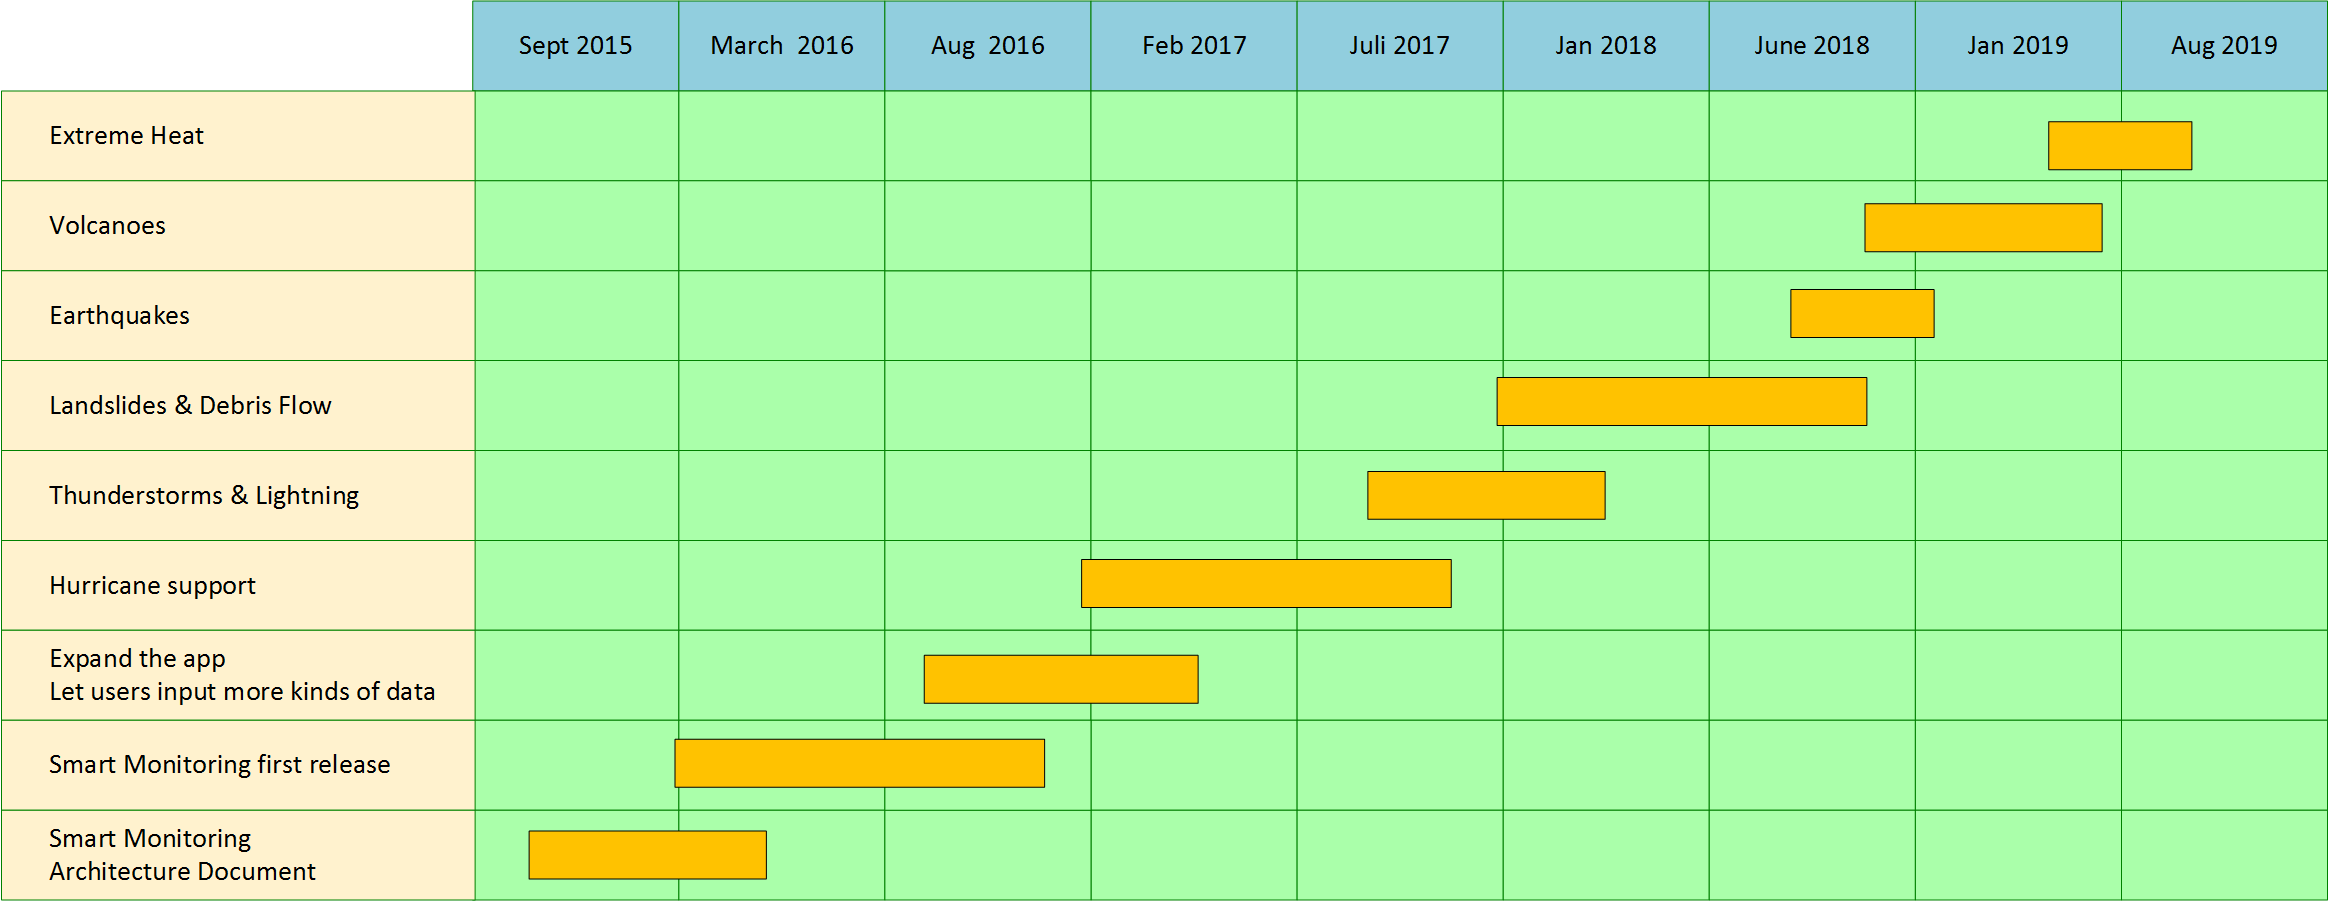
\includegraphics[width=0.95\textwidth]{{{2-business/images/release}.png}}
   \caption{Future releases.}
   \label{fig:future-releases}
\end{figure}

%\ Keuzes maken hier. We moeten hier een plaatje maken dat over tijd eerst ons main product met opties toont en in de toekomst welke extere futures we willen toevoegen

\section{Target audience}
The target audience is where we focus on to market our product. The Dutch Ministry of Infrastructure and the Environment is responsible for floods in the Netherlands. They make the decisions to buy the system. 

The Netherlands is divided into several safety regions. A safety region consists of all the emergency services, municipalities, water boards. They make decisions about how to make their region safer. All those organizations should be seen as the target audience. They must see the benefit of using \CompanyName{}'s Monitoring and Warning system.


%\section{Business model}
%\ Insert a business model diagram
%\section{Domain model}
%\ Internal how our system works?
\section{Financial model}
The financial model will be a low product price. This in order to price the product low in the market. A service description for maintenance will be offered. Also updates will be sold to the customer\\

\subsection{Software Architecture costs}
The software architecture team of \CompanyName consists of six members. Creating the architecture of the project is estimated to take ten weeks. All team members will spend 15 hours a week on the project. This totals $6*10*15=1050$ working hours. Each working hour costs \euro{}150,-. Total spend on the software architecture is \euro{}157.500

\subsection{Development costs}
The development costs are calculated in the table below.\\
\newline
\begin{longtable}{|L{\tw{0.3}}|L{\tw{0.2}}|}
	\toprule
	\textbf{Description} & \textbf{Man hours} \\ \midrule
	Get values from various sensors & 160 \\ 
	Get weather forecasts & 160 \\ 
	Flood prediction algorithm & 3100 \\ 
	Warning messaging system  & 2000 \\ 
	Guidance information system & 1500 \\ 
	Redundancy and fail over systems & 1000 \\ 
	Testing \& debugging & 600 \\ 
	Release build & 250 \\
	Overhead & 1000 \\ 
	Total hours & 9770 \\ \midrule
\end{longtable}

\todo{add talbe refs?}
The above table shows the project needs approximately 9770 hours to develop the system. The development is done by \CompanyName self. Each member of the project team assigned to develop this system is paid \euro{}50 an hour. This results in a development cost of $50*9770=488.550$. As shown in the table below.

\todo{add the duration?}
%Members & 6 \\
%Duration & $\approx$41 weeks \\
\begin{tabular}{L{\tw{0.3}}|L{\tw{0.2}}|}
Hours & 9770 \\
Cost per hour & \euro{}50 \\
Total cost & \euro{}488.500 \\ \bottomrule
\end{tabular}

\subsection{Hardware costs}
Around 17,000 kilometres of dikes protect the Netherlands against flooding \cite{DMC}.
Sensor costs include:
\begin{itemize}
	\item technical costs of the sensor
	\item implementation costs
	\item system implementation costs
\end{itemize}

The system needs:
\begin{itemize}
	\item Sensors
	\item {State monitor server}
	\item {Danger check server}	
	\item {Warning system server}	
	\item {Guidance server}	
\end{itemize}

%Spaargaren2012.pdf. p127, thank god.
\cite{UvAPHD} pp 127.
The first case considers monitoring of the smallest stretch of 6 km with a simple monitoring 
system S1. The monitoring system consists of MEMS sensor modules (e.g. GeoBeads) with a claimed life time of 10 years, which are installed with conventional CPT push-in techniques. Three sensors are installed per cross-section and a cross-section is installed every 100 m. The total installation costs of monitoring system S1 are,


The system uses dyke meters and water meters. The system needs at least 200 water meters and 75 dyke meter. A water meter costs about \euro{}5 and a dkyke meter costs \euro{}60 each. Each server costs \euro{}1.500. This results in the minimum hardware costs of be \euro{}11,500. \\
 However, it is very important that the system doesn't fail. So if a few components or sensors fail, the system should still be fully functional. To make sure the system won't fail if a component fails, the hardware is redundantly set up four times.\\
 The total hardware costs then results in: \euro{}46.000

\subsection{Total costs}
The total costs for the system is calculated in the table below.\\
\newline
\begin{tabular}{|L{\tw{0.3}}|L{\tw{0.2}}|}
	\toprule
	Software Architecture costs & \euro{}157.500\\ \midrule
	Development costs & \euro{}{}488,500\\ \midrule
	Hardware costs & \euro{}46.000\\ \midrule
	Total cost & \euro{}692.000\\
	\bottomrule
\end{tabular}\\
So the total costs for developing the system is \euro{}692.000\\
% Guntur: Doubled financial model sections?
% \section{Financial model}
% The financial model will be a low product price. This in order to price the product low in the market. A service description for maintenance will be offered. Also updates will be sold to the customer

\section{Competitors}
Siemens is a competitor that already has developed a flood-warning system in Belgium in 2006. When the system detects a imminent flood it sends a SMS to people that live near the rivers in order to warn them. The system is implemented in a small region, which consists of only 3 rivers. The total cost for this system were \euro{}230.000. Later on they continued engineering the system. The system uses sensor which measures: temperature, water pressure, and shifting. They participated with this system in the Urban Flood project from the EU. The strong point of this competitor is that they already have funding and also experience with building such a system. Siemens is the main competitor for \CompanyName{}. Their strength is that they already have a proven system in Belgium and have a lot of experience through participating in flood monitoring research projects. The opportunity for \CompanyName{} is Engineering a flexible system that can be used in the future for other kind of disasters. Further on by selling the product at a low selling price and profit on the maintenance work and upgrades the Netherlands will be interesting in using the product.

Further there are Universities that do research on flood warning systems. At the Malaysian Institute Information Technology they developed a product prototype of a system called Intelligent Flood Information System via SMS. Waterlevel sensors are the only one they used. When their is a flood they send a warning SMS to people that are within the area. In the future this could become a competitor if they create a start-up or sell the idea to a company.  



%http://www.researchgate.net/publication/239761436_Intelligent_flood_information_system_via_SMS_(IFIS)

%http://datanews.knack.be/ict/nieuws/sms-waarschuwt-voor-overstromingen-br/article-normal-317597.html
%http://www.urbanflood.eu/Pages/Newsletter6.aspx
%https://en.wikipedia.org/wiki/Flood_warning (examples)
%https://www.campbellsci.com/flood-warning (sensors)


%!TEX root = ../report.tex
\chapter{Requirements}
\label{ch:requirements}
This chapter will describe the vision and use it to derive stakeholders to be able to properly write use cases and stories. These will be used to extract functional, commercial, technical and evolution requirements. Afterwards, a risk assessment will take place, to ensure that the project is not at great risk.
%!TEX root = ../report.tex
\section{Architectural vision}

%!TEX root = ../report.tex
\section{Stakeholders and their concerns}

% wonder where do these factors come from

%kind of QA's (accourding to "Software Requirements" 3rd edition, Karll Wiegers and Joy Beatty)
%from page 263:

This section defines all stakeholders of our system and describe the concerns of the stakeholders. A stakeholder might be a person, group of persons, or organization that are involved in our system. There are eight stakeholders, ranged from first parties to third parties stakeholders. We use several quality standards from "Software Requirements" book by Microsoft \cite{wiegers2013software}. Those quality standards are described in \autoref{table:qa_standard}.

\begin{table}[!htbp] \centering
    \caption{Quality attributes of Software Architecture from "Software Requirements" Book \cite{wiegers2013software}.}
    \label{table:qa_standard}
    \begin{tabular}{L{\tw{0.2}} L{\tw{0.4}}}
    \toprule
    \textbf{Quality Attributes} & \textbf{Brief description} \\ \midrule
    Availability & The extent to which the system's services are available when and where they are needed\\
    Interoperability & How easily the system can interconnect and exchange data with other systems or components\\
    Performance & How quickly and predictable the system responds to user inputs or other events\\
    Reliability & How long the system runs before experiencing a failure \\
    Security & How well the system protects against unauthorized access to the application and its data\\
    Usability & How easy it is for people to learn, remember, and use the system\\
    \bottomrule
    \end{tabular}
\end{table}

There are six quality attributes, as can be seen in \autoref{table:qa_standard}, for measuring stakeholders' concern regarding our system. Furthermore, we also add profitability as another quality standard to improve measuring stakeholders' concern. Detailed description of stakeholders and their concerns are explained below.

% %from page 209 (Software Requirements book from microsoft):
% \todo{quote book, and ISO}
% Book and (ISO/IEC/IEEE 2011):\\
% \begin{tabular}{|L{\tw{0.2}}|L{\tw{0.4}}|}
% \toprule
% \textbf{Keyword} & \textbf{Priority} \\
% Shall & Required \\
% Should & Desired \\
% May & Optional \\
% \bottomrule
% \end{tabular}

\begin{description}
\item[Product owner] is concerned about the reliability and profitability of the system. The product owner funds the whole project and is highly concerned about the profitability. Thus, to gain big market share and extract large profit from this product, the product owner has to make this product reliable.
 
\item[Developers] are concerned about interoperability, performance and security. We, the architect team of RugSAG3 company, are also part of this. This stakeholder is responsible for the development of the systems until it is ready for production. Including architecting, designing, analyzing, testing and implementing this SFM System.

\item[Third party developers] are concerned about interoperability, availability, usability and reliability. Third party developers are important for our system since they need to provide an application that will give the users guidance in case of a flood.

\item[Competitors] are concerned about reliability and profitability. Competitors give negative effect on the system because competitors will be aiming on the same customer target. On the other hand, competitors are also triggering us to make a really good system in order to be able to compete with them and to save more lives. Thus, competitors must also be kept in consideration.

\item[Government] is concerned about availability and reliability. The government will be the main customer of this product, specifically, The Dutch Ministry of Infrastructure and the Environment. The government will be part of mitigation when the flood is imminent. This system will help the government by notifying them when it detects a flood and supplying them with relevant information about the flood.

\item[Citizens] are also concerned about availability and reliability, but also usability, since they can subscribe to warning by SMS. The Dutch residents are indirect user of this systems. Furthermore, they want this system to always be available and run correctly and notify them with reliable information.
% Guntur: I do not know the exact position of insurance companies in our stakeholders. Can anybody explain about this? Or should we just remove this stakeholder?

\item[Insurance companies] are concerned mostly about performance, reliability and availability. The damages caused by flood sometimes are also covered by the insurance companies. Thus, the insurance companies will also be part of the stakeholders and they will make sure that their business is running well.

\item[Local companies] are concerned about availability and reliability. Local companies will also be affected by the flood, since they have a lot of resources which are in danger. Local companies want to know whether or not this system is reliable so that they can arrange a proper action set when the flood comes to save their assets.

\item[Safety region] is responsible for the emergency services and is concerned about interoperability, performance, availability, reliability and usability. Emergency services are important when any accident happens, including flood. They will be really concerned about the thing that makes this system reliable, and inter-operable to their current system.
\end{description}

\autoref{table:stakeholder_concern} illustrates the stakeholder concern matrix. In our approach every stakeholders are equally the same. Thus, each stakeholder receives 100 points in total that has to be distributed among all the concerns.

\begin{table}[!htbp] \centering
	\caption{Matrix of stakeholders concern.}
	\label{table:stakeholder_concern}
    \begin{tabular}{@{} cl*{11}c @{}}
        &  & \multicolumn{7}{c}{\textbf{Concerns}} \\[2ex]
        & \textbf{Stakeholder} & \rot{Weight} & \rot{Availability} & \rot{Interoperability} & \rot{Performance} 
        & \rot{Reliability} & \rot{Security} & \rot{Usability} & \rot{Profitability}\\
        \cmidrule[1pt]{2-10}		
                     %   	   weight ava inte perf reli sec  usa  prof
        & Product owner			& 1	&    &    &    & 60 &    &    & 40 \\
        & Developers			& 1	& 	 & 40 & 30 & 	& 30 &    &    \\
        & Competitors 			& 1	&    &    &    & 40 & 	 &    & 60 \\
        & Government 			& 2	& 60 & 	  &    & 40 &    &    &    \\
        & Citizens				& 2	& 40 &    &    & 40 &    & 20 &    \\
        & Insurance companies	& 1	& 35 &    & 15 & 50 &    &    &    \\
        & Local companies		& 1	& 60 &    &    & 40 &    & 	  &    \\
        & Safety region			& 3	& 20 & 15 & 20 & 30 &    & 15 &    \\
        \cmidrule{2-10}
        & Total                	&	& 355& 85 & 105& 440& 30 & 85 & 100\\
        \cmidrule{2-10}
    \end{tabular}
\end{table}

As can be seen from \autoref{table:stakeholder_concern}, the most important concern of our system is the reliability, following availability as the second most important concern. This is also identical with our significant key driver.


% Key drivers
% high level requirements

%!TEX root = ../report.tex

%Citizen subscribes to service
%Sensor data is retrieved FR-1, FR-3, FR-5
%Weather data is retrieved FR-7
%Predict floud probability FR-8
%Get geo data FR-9
%The system should predict water levels FR-11, FR-12
%Monitor people should have access to a control panel FR-21

\clearpage


\section{Stories and use-cases}
This section will give an overview of the different use-cases. Figure \ref{fig:usecase-diagram} displays the use-case diagram. This provides an overview of the use-cases with their actors. In the subsections below, the architectural important use-cases are explained in more detail.

\begin{figure}[H]
	\centering
	\includegraphics[scale=0.35]{images/usecaseDiagramNew.png}
	\caption{Use-case diagram}
	\label{fig:usecase-diagram}
\end{figure}


%slides say:
%	Name & \\
%	Number & \\
%	Primary actor &  \\
%	Scope &  \\
%	Level &  \\
%	Extensions &  \\
%	Sub-variations & \\


\subsection{Receive sensor data}
\pgfplotstabletypeset[%
	UCTable
]{%
	value & description \\
	Number & \req{uc}\\
	Description & The system receives data from the different sensors deployed \\
	Stakeholders and interests & 
	\textbf{Developers}: Developers need to work with the sensor data \\
	Primary actor & System\\
	Scope & Monitoring part of the system \\
	Level & Sub process\\
	Precondition & The sensor is connected to a processing unit \\
	Main success scenario & \compactList{enumerate}{%
		\item The sensor does a measurement every 10 seconds
		\item The sensor sends the data to the central server every minute
		\item The central server normalizes the received data
		\item The central server stores the normalized data to the database
		\item The database stores the data
		}\\
	Postcondition & The database received and stored the sensor data \\
	Alternatives & \compactList{itemize}{%
		\item[2a.] 
		\begin{enumerate}
			\item The data cannot be sent
			\item Data will be lost
			\item The use-case ends 
		\end{enumerate}
		} \\
	Related requirements & \ref{fr:receive-waterlevel}, \ref{fr:receive-pressure}, \ref{fr:store-sensordata}, \ref{fr:retrieve-sensordata}\\
}

\clearpage
\subsection{Receive weather/GEO data}
\pgfplotstabletypeset[%
	UCTable
]{%
	value & description \\
	Number & \req{uc}\\
	Description & The system receives data from the weather forecast service \\
	Stakeholders and interests & 
	\textbf{Developers}: Developers would like to have a simple to use API \\
	Primary actor & System\\
	Scope & Monitoring part of the system \\
	Level & Sub process\\
	Precondition & The system needs external weather data to predict floods \\
	Main success scenario & \compactList{enumerate}{%
		\item The processing unit determines it needs forecast weather data%
		\item A call is made to the weather forecast service%
		\item The weather forecast service returns the requested data
		}\\
	Postcondition & The system received the forecast data \\
	Alternatives & \compactList{itemize}{%
		\item[3a.] 
		\begin{enumerate}
			\item The data cannot be returned.
			\item Repeat this process with another weather forecast service.
			\item If none are available, proceed monitoring without weather forecast data.
			\item After 5 minutes try to reconnect.
		\end{enumerate}
		}\\
	Related requirements & \ref{fr:receive-weather}\\
}

\clearpage
\subsection{Subscribing to SMS Service}
\pgfplotstabletypeset[%
	UCTable
]{%
	value & description \\
	Number & \req{uc}\\
	Description & Citizens can subscribe to the SMS service, so when a flood happens they will get a direct text message\\	
	Stakeholders and interests & 
	\textbf{Citizens}: Citizens want to be warned as soon as possible.
	\\
	Primary actor & Citizen\\
	Scope & Warning part of the system \\
	Level & User goal \\
	Precondition & Citizen has a mobile phone and is not subscribed to the SMS service \\
	Main success scenario & \compactList{enumerate}{
		\item Citizen sends a text message to our SMS service
		\item The SMS service receives the text message
		\item The SMS service sends the phone number to the SFM system
		\item The SFM system stores the phone number in the database
		\item A text message is sent back to the citizen with confirmation by the SMS service
		}\\
	Postcondition & Citizen is subscribed to the SMS service \\
	Alternatives & \compactList{itemize}{%
		\item[2a.] The text message is not received \\
		The use-case ends
		}\\
	Related requirements & \ref{fr:citizens-subscribe} \\
}

\clearpage
\subsection{Determining flood probability}
\pgfplotstabletypeset[%
	UCTable
]{%
	value & description \\
	Number & \req{uc}\\
	Description & The central processing unit calculates the probability of a flood \\
	Stakeholders and interests & \compactList{itemize}{%
		\item \textbf{Safety region}: The safety region wants to know when a flood warning is triggered
		\item \textbf{Government}: The government would also like to know when a flood warning is triggered
		}\\
	Primary actor & System\\
	Scope & Monitoring and warning part of the system\\
	Level & Sub process\\
	Precondition & The sensor data is available \\
	Main success scenario & \compactList{enumerate}{%
		\item The central processing unit gets the latest sensor data from the database
		\item The central processing unit gets the latest weather forecast data
		\item The central processing unit calculates the probability of a flood
		\item The central processing unit stores the probability value in the database
		\item The central processing unit determines that a flood is imminent based on the probability value
		\item A warning is send to the emergency services (they will warn the government)
		\item A warning is send to the citizens
		}\\
	Postcondition & The flood probability is calculated and stored. If the probability exceeds a certain threshold, a warning is sent to the authorities and citizens \\
	Alternatives & \compactList{itemize}{
		\item[5a.] The probability is not above the threshold \\
		The use-case ends
		}\\
	Related requirements & \ref{fr:detect-flood} \\
}

\clearpage
\subsection{Warn citizens in case of an imminent flood}
\pgfplotstabletypeset[%
	UCTable
]{%
	value & description \\
	Number & \req{uc}\\
	Description & Citizens who are subscribed to the SMS service will be warned through text messages in case of an imminent flood\\	
	Stakeholders and interests & \compactList{itemize}{
		\item \textbf{Citizens}: When they are subscribed, they want to be warned in case of an imminent flood
		}\\
	Primary actor & Citizen\\
	Scope & Warning part of the system \\
	Level & User goal \\
	Precondition & There is an imminent flood and the citizen is subscribed to the SMS service\\
	Main success scenario & \compactList{enumerate}{%
		\item The flood monitoring \& detection unit sends a warning about an imminent flood to the warning unit
		\item The warning unit queries the database for a list of phone numbers of subscribed citizens in the area
		\item The monitoring unit sends the collected phone numbers to the SMS service
		\item The SMS service sends a warning to all the collected phone numbers
		}\\
	Postcondition & The citizens who are subscribed received a warning\\
	Alternatives & \compactList{itemize}{%
		\item[3a.] 
		\begin{enumerate}
			\item A message cannot be sent to the citizen
			\item Wait a minute and resend
			\item The use-case ends
		\end{enumerate}
		}\\
	Related requirements & \ref{fr:warn-citizens} \\
}

\clearpage
\subsection{Warn safety region in case of an imminent flood}
\pgfplotstabletypeset[%
	UCTable
]{%
	value & description \\
	Number & \req{uc}\\
	Description & The safety region needs to receive a warning about an imminent flood\\
	Stakeholders and interests & \compactList{itemize}{%
		\item \textbf{Government}: The government wants to warn the citizens in case of a flood
		\item \textbf{Safety regions}: The emergency services want to help the citizens in case of a flood
		}\\
	Primary actor & Safety region \\
	Scope & Warning part of the system \\
	Level & User goal \\
	Precondition & There is an imminent flood\\
	Main success scenario & \compactList{enumerate}{
		\item The processing unit determines what area will be under water in case of a flood
		\item The processing unit determines how many people will be affected by the imminent flood
		\item The processing unit predicts how the flood will develop in the following period 
		\item The processing unit will create a map based on the current state and predictions
		\item The processing unit sends the map to the government and emergency services
		}\\
	Postcondition & A map with current and predicted data is sent to the government and emergency authorities \\
	Related requirements & \ref{fr:compute-area}, \ref{fr:analyze-waterlevel}, \ref{fr:estimate-waterlevel}, \ref{fr:compute-nrcivilians}, \ref{fr:warn-safetyregion} \\
}

\clearpage
\subsection{Third party accessing data through the systems API}
\pgfplotstabletypeset[%
	UCTable
]{%
	value & description \\
	Number & \req{uc}\\
	Description & Third parties can use the API exposed by the flood monitoring system in third party applications (providing guidance to citizens) \\
	Stakeholders and interests & \compactList{itemize}{%
		\item \textbf{Third parties}: Third parties want to access the data of the flood monitoring system to use in their applications
		\item \textbf{Citizens}: Citizens want to receive guidance in case of a flood.
		}\\
	Primary actor & Third party \\
	Scope & The API part of the system \\
	Level & User goal \\
	Precondition & The third party has access to the flood monitoring systems API \\
	Main success scenario & \compactList{enumerate}{
		\item The third party application connects to the API
		\item The third party application sends a request for certain data to the API
		\item The system retrieves the requested data from the database
		\item The system sends the retrieved data to the third party application
		}\\
	Postcondition & The third party application has received the requested data \\
	Related requirements & \ref{fr:expose-api} \\
}

\clearpage
\subsection{Detecting a faulty sensor}
\pgfplotstabletypeset[%
	UCTable
]{%
	value & description \\
	Number & \req{uc}\\
	Description & The system is able to detect when a sensor is not functioning properly \\
	Stakeholders and interests & \compactList{itemize}{%
		\item \textbf{Product owner}: The product owner wants the system to be reliable and errors/broken sensors to be fixed
		}\\
	Primary actor & The system \\
	Scope & The monitoring part of the system \\
	Level & Sub process \\
	Precondition & The sensor is not functioning properly \\
	Main success scenario & \compactList{enumerate}{
		\item The system receives the sensor data
		\item The system compares the sensor data with other information, including data of nearby sensors and previous data of this sensor 
		\item The system detects that this reading is abnormal, but determines it cannot be caused by an (imminent) flood
		\item The system ignores further readings from this sensor and reports the faulty sensor in the control panel
		}\\
	Postcondition & The faulty sensor is not used in future measurements and is reported in the control panel \\
	Alternatives & \compactList{itemize}{%
		\item[3a.] 
		\begin{enumerate}
			\item The system cannot determine the abnormal reading is not caused by a flood
			\item The system keeps using this sensors data, until it can determine that the readings are not caused by a flood, or it determines that it is caused by a flood (in which case it will issue warnings, see \hyperref[uc:4]{UC-4})
		\end{enumerate}
		}\\
	Related requirements & \ref{fr:detect-faultysensor}, \ref{fr:report-faultysensors}, \ref{fr:controlpanel-warnings}, \ref{fr:controlpanel-errors}, \ref{fr:controlpanel-sensors}
	\\
}

\clearpage
\subsection{Maintenance employee checks system state}
\pgfplotstabletypeset[%
	UCTable
]{%
	value & description \\
	Number & \req{uc}\\
	Description & A maintainer of the system regularly checks the state of the system in the control panel to see if there are errors or sensors that need maintenance. \\
	Stakeholders and interests & \compactList{itemize}{%
		\item \textbf{Product owner}: The product owner wants the system to be reliable and errors/broken sensors to be fixed
		}\\
	Primary actor & Maintainer \\
	Scope & The maintenance part of the system \\
	Level & User goal \\
	Precondition &  \\
	Main success scenario & \compactList{enumerate}{
		\item The maintainer uses his login credentials to get access to the control panel
		\item The maintainer navigates to the errors/warning page
		\item The maintainer checks on this page if there are problems with the system (errors/warning)
		\item The maintainer takes necessary action to resolve any issues
		}\\
	Postcondition & The maintainer is aware of reported problems with the system \\
	Related requirements & \ref{fr:controlpanel}, \ref{fr:report-faultysensors}, \ref{fr:controlpanel-warnings}, \ref{fr:controlpanel-errors}, \ref{fr:controlpanel-sensors} \\
}



%!TEX root = ../report.tex
\section{Functional requirements}
\begin{longtable}{p{0.1\textwidth} p{0.1\textwidth} p{0.8\textwidth}}
    \textbf{Nr.} & \textbf{Prio}  & \textbf{Description} \\
    
    \hline \phantomsection \label{fr:1} FR-1 & 
    \phantomsection  \textbf{Must} &
    \phantomsection  The system is able to receive and process input from sensors with regards to the water level. This information will be used to determine if there is an imminent flood. \\
    
    \hline \phantomsection \label{fr:2} FR-2 & 
    \phantomsection  \textbf{Must} &
    \phantomsection  The system is able to receive and process input from sensors with regards to the pressure/consistency of the dykes. This information will be used to determine if there is an imminent flood. \\
    
    \hline \phantomsection \label{fr:3} FR-3 & 
    \phantomsection  \textbf{Must} &
    \phantomsection  The system retrieves weather forecasting data from weather forecasting services. The retrieved weather forecasting data consists of predictions about the precipitation and wind data. This data will be used by the system to help in determining when a flood becomes imminent.
     \\
     
    \hline \phantomsection \label{fr:4} FR-4 & 
    \phantomsection  \textbf{Must} &
    \phantomsection  The system is able to detect from the sensor data and weather forecast information when a flood is imminent. \\ % what are the criteria for an imminent flood??
    
    \hline \phantomsection \label{fr:5} FR-5 & 
    \phantomsection  \textbf{Must} &
    \phantomsection The system can compute (from geographic information) the area which will be affected by a flood. \\
    
    \hline \phantomsection \label{fr:6} FR-6 & 
    \phantomsection  \textbf{Must} &
    \phantomsection The system is able to collect information pertaining to the severity of the flood. The severity can be deducted from the expected water level, how fast the water level in the flood area will rise, and by the number of civilians living in the affected area (population density). \\
    
    \hline \phantomsection \label{fr:7} FR-7 & 
    \phantomsection  \textbf{Must} &
    \phantomsection The system provides emergency services with information about the flood. This includes the area affected by the flood and information needed to deduct the severity of the flood. \\
    
	\hline \phantomsection \label{fr:8} FR-8 & 
    \phantomsection  \textbf{Must} &
    \phantomsection  When a flood is imminent, the system should send a warning to the emergency services and to the authorities.\\
    % what info is in the warning
    % who is that: authorities?
    
    \hline \phantomsection \label{fr:9} FR-9 & 
    \phantomsection  \textbf{Must} &
    \phantomsection  The system is able to compute a safe route to a safe area where citizens can be evacuated to in case of an (imminent) flood. \\    

    \hline \phantomsection \label{fr:10} FR-10 & 
    \phantomsection  \textbf{Must} &
    \phantomsection  When a flood is imminent, the system should send a warning to citizens who are subscribed for such warnings. This warning will contain information about how to get to a safe area. \\
	
    \hline \phantomsection \label{fr:11} FR-11 & 
    \phantomsection  \textbf{Must} &
    \phantomsection  The system is able to predict the development of the water level. This information can be used to predict how fast a flood will develop. \\
	
    \hline \phantomsection \label{fr:12} FR-12 & 
    \phantomsection  \textbf{Must} &
    \phantomsection The system uses different sources to confirm imminent flood warnings, in order to limit false positives. \\% not very specific yet
	
    \hline \phantomsection \label{fr:13} FR-13 & 
    \phantomsection  \textbf{Must} &
    \phantomsection The system can detect a faulty sensor, either when the sensor raises an error or when the data from the sensor is inconsistent with other sensor data. \\
	
    \hline \phantomsection \label{fr:14} FR-14 & 
    \phantomsection  \textbf{Must} &
    \phantomsection The system can report faulty sensors, so these sensors can be repaired or replaced. \\ %how will it be reported and to whom?? \\
    
	\hline \phantomsection \label{fr:15} FR-15 & 
    \phantomsection  \textbf{Must} &
    \phantomsection In case of a flood, the system will provide emergency services with safe routes to incident locations. \\
    
    \hline \phantomsection \label{fr:16} FR-16 & 
    \phantomsection  \textbf{Must} &
    \phantomsection Citizens are able to subscribe to flood warning messages. \\
    % TODO: we need to decide how citizens will subscribe: web page, app??
    
    \hline \phantomsection \label{fr:17} FR-17 & 
    \phantomsection  \textbf{Must} &
    \phantomsection The system has access to geographic information, including road data and terrain height data. \\
    
    \hline \phantomsection \label{fr:18} FR-18 & 
    \phantomsection  \textbf{Must} &
    \phantomsection The system can determine the area affected by a flood, by using the location data of the sensors and geographic information. \\
    
    \hline \phantomsection \label{fr:19} FR-19 & 
    \phantomsection  \textbf{Must} &
    \phantomsection The system can determine the location of the citizen, after he/she is warned about a flood, in order to compute a safe route to a safe area. \\
    
    \hline \phantomsection \label{fr:20} FR-20 & 
    \phantomsection  \textbf{Must} &
    \phantomsection The system can determine the location of an emergency vehicle, so it is able to compute a safe route to incident locations. \\
    
    
	
    \hline \phantomsection \label{fr:21} FR-21 & 
    \phantomsection  Future &
    \phantomsection The system is able to detect extreme weather phenomena, like storms etc. \\
\end{longtable}

%!TEX root = ../report.tex
\section{Commercial non functional requirements}
 In this section commercial non functional requirements are presented.
 
\textbf{CNFR-1} The system is affordable.
The selling price of the system to the authorities is about *********** euros per city or municipality. This price is lower than 70\%\ of the competitors price. % How to calcuatenthe selling price , do we need to give it ?

%\textbf{CNFR-2} The maintenance costs are ********** euros.

\textbf{CNFR-2} The sensors have a good quality , the sensors companies have good ratings so we don't have replace the sensors often => less money spent on repairs. The guarantee of the sensors should be about three years.

IDEAS :
\textbf{CNFR-} A video explains how the system works to the end-users : authorities and emergency services.
\textbf{CNFR-} Advertissement ???

%!TEX root = ../report.tex
\section{Technical non-functional requirements}
In this section, the technical non-functional requirements important to this system are discussed.

\subsection{Resilience}
The system will have many connected sensors, which can have failures. The system should be able to recognize such failures timely and recover from them without the QoS or the functionality of the system being affected. 

The system should be able to continue functioning with the same QoS in a situation where up to 5\% of the sensors suffer from failures.  % WM: is 5% realistic?

\subsection{Interoperability}
The system has dependencies on third-party systems. For example, to make predictions about the development of waterlevel, the system will need to retrieve information from water forecasting services. 

Not only for input, but also for output, the system will need to interoperate with third-party systems. If the system has registered a risk of a flood, it should interact with systems of emergency services and other authorities to alert them and sent relevant information.
% TODO: how to measure? 

% ============================================================
% From Gerrit:
% The three main requirements:
% 1: Monitoring activities: the system should monitor activities and properties of
% rivers, waterways, dykes, such as the water level and pressure or the consistency
% of the dyke. Monitoring can be performed through different devices, e.g. analog
% and digital sensors, Unmanned Aerial Vehicles (UAVs) and Vehicular Ad-hoc
% Networks (VANETs) etc.
% 2: Warning: in case of an imminent flood, the system should issue warnings to the
% authorities and emergency services, but also directly to citizens who are
% subscribed for such messages (e.g. through SMS or mobile apps).
% 3: Guidance: the system should provide runtime information to guide its
% constituents or third parties, .e.g. the UAVs may provide information to
% VANETs embedded in vehicles crossing the area, thereby guiding vehicles
% driving towards a flood area to avoid certain routes. Meanwhile, the VANETs
% can also provide an alternative route to emergency services or citizens to avoid
% the flood area. 

% ToDo:
% Stakeholders
% Use-cases
% Make them smart
% Assign value (must/should/...
% ============================================================


%!TEX root = ../report.tex}
\section{Evolution requirements}
%\label{subsec:evolrequir}

%Typical change-cases with respect to the environement, the features and the technology of the system
%http://www.agilemodeling.com/artifacts/changeCase.htm
When establishing the project, architects of the system listed a certain number of requirements which describe the features of the system. However, due to environmental changes and changing stakeholder interests, for example, the requirements may evolve.

%\textbf{ER-1 : Changes in the display of the map } \\
%\textit { Evolution of \ref{fr:construct-map}}. Citizens who subscribed for flood warnings get a map with specific route information (according to their location) to a safe area through the API. \\

%\begin{longtable}{L{0.1\textwidth} L{0.12\textwidth} L{0.7\textwidth}}
	%\textbf{Nr.} & \textbf{Name}  & \textbf{Description} \\


\textbf{ER-1 : Adding of external input}\\
 Citizens can contribute to the guidance by giving extra information (for example if they identified a safe route near their location). This information can be checked by an operator (thanks to photograph by the UAVs for example). 
 
 Functionality can be added to the system in the future, that can take citizen feedback into account for the flood prediction.
 \\
 
\textbf{ER-2 : New sensors } The system is able to work with new sensors technologies, which are coming on the market over the years. \\

\textbf{ER-3 : Improved algorithms for detecting a flood} \\
New algorithms may become available, which have a better accuracy for the flood prediction described in \ref{fr:detect-flood}. The part of the system with the flood prediction algorithm has to be modular, so that it can be replaced with an improved algorithm, once such an algorithm becomes available.

	%\bottomrule
%\end{longtable}


%\textbf{ER-3 : New OS } \\
%The system is able to work with other operating systems than Linux, for example Windows and MacOS. %Portability

%\textbf{ER-3} The system is able to work on several mobile devices platforms : Android, iOs, Windows Phone. \\ IN CASE OF AN APP

%!TEX root = ../report.tex
\newpage
\section{Risk assessment}
\label{sec:risk-assesment}
The system is confronted by several risks which are determined and mitigated in this section.
Taking those risks into account allows to avoid them or at least reduce their impact. 
The risk management involves the identification of the risks, their probability and potential impact or consequences.

The tables below explain the meaning of the definition for probability and consequence.
\begin{figure}[H]
	\centering
	\begin{tabular}{|c|c|}
		\hline \textbf{Probability} & \textbf{Likelihood of occurrence} \\ 
		\hline High                 & 0.65 - 1.00                       \\ 
		\hline Medium               & 0.35 - 0.65                       \\ 
		\hline Low                  & 0.00 - 0.35                       \\ 
		\hline
	\end{tabular} 
	\label{table:risk-probability}
\end{figure}

\begin{figure}[H]
	\centering
	\begin{tabular}{|l|p{15.5cm}|}
		\hline \textbf{Severity} & \textbf{Explanation}                                                                                                                        \\ 
		\hline Severe            & A risk that can lead to loss of live or casualties.                                                                                         \\ 
		\hline Significant       & A risk that can lead to damages, can delay the project more than 3 months or causes one of the high-level requirements not to be fulfilled. \\ 
		\hline Moderate          & A risk that can lead to one of the high-level requirements not to be fulfilled to an acceptable level.                                      \\ 
		\hline Minor             & A risk that can lead to one of the high-level requirements not being fully fulfilled, but still fulfilled in an acceptable level.           \\
		\hline
	\end{tabular} 
	\label{table:risk-severity}
\end{figure}

%Risk impact assesment and Prioritization
% Probability of Occurrence ( In the appendice is the table to which show how to evaluate a risk and the severity of consequences 
%\textit{http://www.mitre.org/publications/systems-engineering-guide/acquisition-systems-engineering/risk-management/risk-impact-assessment-and-prioritization} \\ % COSTS
%Timeframe is classified in : Long , Medium , Short , Imminent \\
%Consequences are classified in : Low, Moderate , High , Severe


%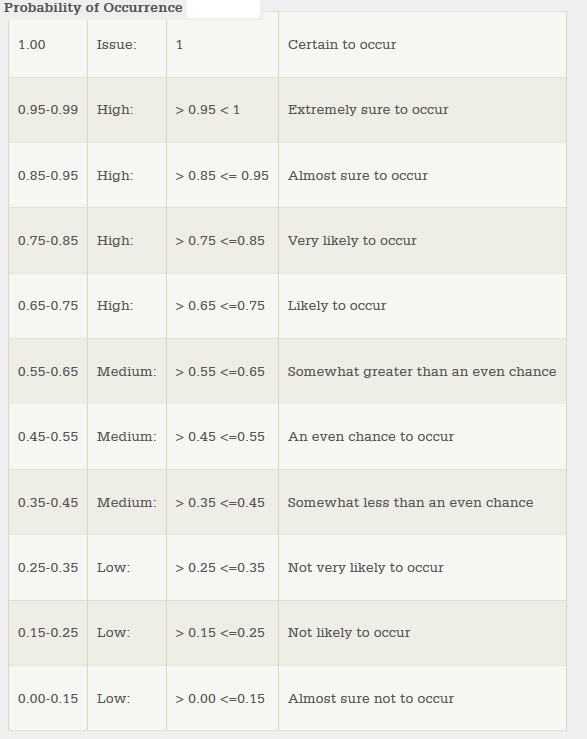
\includegraphics[scale=0.5]{3-requirements/Images/RISKSOCCURENCE.jpg} % maybe in the appendice ?
\subsection{Technical}

\risk{T}
{The system does not detect a flood}
{Low}
{Severe. There can be a loss of human lives and damages, loss of trust in the system by end-users.}
{Make sure the number of sensors is sufficient and that they are in good state (as low failure rate as possible, when necessary repair or replace them). Perform regular checks of the sensors. Make sure faults in sensors are reported. }
{Make changes in the algorithm for the flood detection, add more and new sensors which have good rates according to quality tests.}
{risk:flood-detect}

\risk{T}
{The system sends warnings of a non-existing flood (false positive)} % WHEN THERE IS A FLOOD YOU KNOW IT
{Low}
{Significant. People can become more negligent to future messages and unneeded social disturbance can be caused.}
{UAVs watching the area where the supposed flood is to confirm.}
{Send a message as soon as the mistake is detected to tell the population/emergency center it was a false alert. }
{risk:warning-nonexisting}

\risk{T}
{The system cannot send messages to the necessary people because the communication platform is also destroyed by the flood}
{Medium}
{Severe. If the warning is not send, the area might not be evacuated timely. Potential loss of human lives, casualties and damages to property. }
{}
{Send the warning to the safety board using a different medium.}
{risk:cantwarn}
	
\risk{T}
{The config panel is not checked often enough and broken sensors are not fixed}
{Low}
{Moderate. The accuracy and reliability of the system diminish if less sensors are available to the system.}
{Make sure there is a clear schedule for maintenance personnel to check the control panel.}
{Repair/replace all the sensors which were not repaired timely}
{risk:configpanel-notchecked}
	
%\risk{T}
%{The system sends incorrect information}
%{Low}
%{Severe. Loss of money and maybe lives.}
%{Operator checking the validity of the information sent by the system.
%	Good collaboration with the insurance companies.}
%{  }
% WM: Risk and severity depend highly on what kind of information is send incorrectly.

\risk{T}
{Hacker gets access to the system}
{Low}
{Severe. The hacker may sent incorrect information deliberately during the flood. This can cause unneeded evacuation, but in the case of a flood also loss of human lives. The system is not reliable anymore.}
{Change password and hash codes every three months. Hire specialists in the security field to audit the security system on a regular basis (penetration testing).}
{Update the security system / change it. Find a new algorithm for the creation of password and hash codes.}
{risk:hacker}

\risk{T}
{UAV cannot fly because of the weather}
{Medium}
{Moderate. If the UAV cannot fly, the system cannot use the data it would have collected for the flood probability computation.}
{Bad weather cannot be prevented. Use UAVs which can fly in suboptimal weather conditions.}
{If the UAV really cannot fly and the system is not sure about the flood probability, lower the threshold for warning safety region/citizens.}
{risk:uav-badweather}

\risk{T}
{Arduino becomes unavailable}
{Low}
{Minor. The Arduino has a limited number of attached sensors, so the consequences of a single Arduino failures are not too large.}
{Install the Arduino in such a way, that it is not exposed to external forces (like bad weather). This will decrease the odds of an Arduino failure.}
{The broken Arduino is reported in the control panel (several failing sensors) and should be replaced/repaired by maintenance personnel.}
{risk:arduino-broken}

\risk{T}
{SMS Service goes offline when there is a flood}
{Low}
{Moderate. The SMS Service is essential to warn citizens, which is a significant part of high-level requirement \ref{HL:2}.}
{Make sure the SMS Service which is used has good availability guarantees.}
{Use an alternative SMS Service or coordinate with the SMS Service provider to get the service back online.}
{risk:sms-service-online}



\subsection{Business}

\risk{B}
{Wrong estimation of the budget}
{Medium}
{Significant. The final product does not have the features expected.}
{The team needs an accountant or at least someone taking care of the follow-up of the money. Make sure there are regular evaluations to keep track of the money flow.}
{Remove some requirements or features of the product, or change the hardware components used.}
{risk:budget}

\risk{B}
{The money invested in the fabrication and achievement of the product/system is not covered by the sales (shortfall/deficit)}
{Medium}
{Moderate. Stopping the sale}
{The team needs an accountant or at least someone taking care of the follow-up of the money.}
{Adding more features to the product in order to make it more competitive in the market.}
{risk:shortfall}

\risk{B}
{Third-party developers do not build third-party applications using the systems API}
{Medium}
{Moderate. Without third-party applications, the citizens do not receive guidance in case of a flood}
{ Make sure the API exposes all features which are relevant to develop a third-party application for guidance. }
{ Promote the use of the API by third-party developers using, for example, a contest. }
{risk:3rdparty}

%\risk{B}
%{Competitors lowering their prices}
%{Medium}
%{Moderate. Loss of money.}
%{  }
%{  }
% WM: I think this one is too generic
	
\risk{B}
{Sensor becomes unavailable (is not sold anymore)}
{Medium}
{Moderate. Sensors will fail and need replacing over time, if new sensors are not available anymore, this becomes impossible.}
{ Choose a sensor that is not too old and is expected to be available for at least the next 5 years. }
{ Use a different sensor and modify the system so it can operate with this sensor. }
{risk:sensor-notsold}

%\textbf{ B-RISK4 The sensors company become bankrupt or at least stops its sales.} \\
%\textit{Probability of Occurence}: Low \\
%\textit{Consequences}: High.\\
%\textit{Prevention} Our system use sensors from different companies \\
%\textit{Decision}: Find another company selling sensors and make sure of its reliability. \\


\subsection{Schedule}
\risk{S}
{The project is not finished at the deadline}
{Low}
{Significant. Pressure for all the team members, loss of credibility regarding the customers, selling a product with less features than expected.}
{ SRA , Schedule Risk analysis : Estimation of the duration of the project by its manager ( with the use of probability and statistics ) . Meeting for the team members every week to keep track of the timing and take decisions according to the deadline. }
{ Postpone the deadline or remove some features when the deadline can't be postponed. }
{risk:schedule}


%!TEX root = ../report.tex
\chapter{Analysis}
\label{ch:analysis}
This chapter describes the analysis. It lists the assumptions made about the system and it's environment. Next, an overview of the high-level design decisions is given.

\section{Assumptions}
There are several assumptions made about the system and it's environment:

\noindent{
	\begin{enumerate}
	  \item The safety region / government has means to alert citizens in an area to evacuate.
	  \item The safety region is informed about our system and will alert citizens if needed when our system alerts the safety region.
	  \item People who are subscribed for flood warnings/guidance have a mobile phone that can receive text messages and MMS.
	  \item Sensors can be placed in the water ways and dikes in locations where they can provide representative measurements.
	  \item Information is available to the system with regards to the population density and terrain height in different areas.
	  \item A flood will not reach further than 50 km. % see SEC-7
	  \item Supplying information about the areas affected by the flood in a resolution of 5 by 5 km (as described in \ref{fr:10}) is sufficient for the government/safety region to make decisions regarding alerting and evacuating citizens.
	  \item It is possible to predict the expected water level up to 12 hours in the future.
	  \item A weather forecasting API is available that provides precipitation and wind data.
	  \item The sensors are (in some way) connected to the system.
	  \item The safety region provides an API, which can be used by the system to warn the safety region.
	\end{enumerate}
}

\newpage
\section{High-level Design Decisions}
This section discusses the high-level design decisions.

Each decision is explained in a table. The arguments section of the table lists for each alternative a score for every important quality attribute.
A higher score means a more favourable result. For example, a high score for costs means a low cost for the system.
\\[1.0cm]

%\noindent{
%	\begin{itemize}
%	\item Security? (What if someone tries to manipulate a sensor?)
%	\item One or multiple warning systems (failover)
%	\item Networking? Redundancy of cables (trunked?)
%	\item When to alarm? What to do if only 1 sensor warns about a flood?
%	\item Security decisions?
%	\item Operating system decision
%	\item Storage decision
%	\item Push or pull updates? (Pushing I’m hoping)
%	\item Programming language(s) for the system? Web-interface, sensor monitoring, weather forecasting system, push notification system
%	\item In what ways will the system detect a flood? Sensors, UAV’s, forecasting?
%	\item How to detect a flood based on the forecasting? Warn beforehand? Pay extra attention to the new upcoming flood by sending extra robots/uav's?
%	\end{itemize}
%}

% Template for decision table:
% We removed the status from the orignal entry, because we do not use this document to get confirmation on our decisions
% \begin{table}
% \begin{tabular}{L{0.2\textwidth} L{0.6\textwidth}}
%     \textbf{Name} 			& \textbf{Topic} \\ \toprule
%     \textbf{Decision} 		& \textbf{DEC-}\textbf{\nextNrRef{dn}} \\ \midrule \midrule
%     \textbf{Problem/Issue} 	& A problem description \\ \midrule
%     \textbf{Decision} 		& The method/product that has be chosen and why\\ \midrule
%     \textbf{Alternatives} 	& \textit{Other option}\\ 
%     							& Details about the other options\\\midrule
%    \textbf{Arguments} 		& A short discussion of the cons and pro's supported by the table below\\
%    						& 	\begin{tabular}{l|lllllll|l}
% 							& 		\rot{Reliability} & \rot{Resilience} & \rot{Performance} & \rot{Interopertability} & \rot{Security} & \rot{Scalability} & \rot{Cost} & \rot{\textbf{Score}} \\ \hline 
% 									weight 				& ? & ? & ? & ? & ? & ? & ? & ?\\ \hline
% 									Mobile broadband 	& ? & ? & ? & ? & ? & ? & ? & ?\\
% 									landline 			& ? & ? & ? & ? & ? & ? & ? & ?\\
% 									satalite 		 	& ? & ? & ? & ? & ? & ? & ? & ?\\
% 									direct lines 		& ? & ? & ? & ? & ? & ? & ? & ?\\
% 								\end{tabular} \\ \bottomrule
% \end{tabular}
% \caption{Decision -- Decision name.}
% \label{table:caption_alias}
% \end{table}

\begin{table}[h]
\begin{tabular}{L{0.2\textwidth} L{0.6\textwidth}}
    \textbf{Name} 			& \textbf{Linux} \\ \toprule
    \textbf{Decision} 		& \textbf{DEC-}\textbf{\nextNrRef{dn}} \\ \midrule \midrule
    \textbf{Status} 		& \textbf{New} \\ \midrule
    \textbf{Problem/Issue} 	& The warning system software for the natural disasters need a platform to work on.  \\ \midrule
    \textbf{Decision} 		&  The warning system will use Linux as a platform. Based on Unix, Linux is a free platform that has proven itself and is used by many servers. It's open source meaning that everyone can check out how it works.\\ \midrule
    \textbf{Alternatives} 	& \textit{Windows}\\
    						& Operating system is a closed platform developed by one of the biggest tech companies who provide a big development environment with it.\\
    						& \textit{OpenBSD}\\
    						& A Unix-based system that is famous for it's proactive security and runs most of the Linux applications. However, some software packages aren't certified to run on OpenBSD, but are for Linux.\\
    						\midrule
    \textbf{Arguments} 		& \\
    						& 	\begin{tabular}{l|lllllll|l}
							& 		\rot{Reliability} & \rot{Resilience} & \rot{Performance} & \rot{Interopertability} & \rot{Security} & \rot{Scalability} & \rot{Cost} & \rot{\textbf{Score}} \\ \hline
							% 							rel res perf int sec sca cost
									Weight 				& 1 & 1 & 1 & 1 & 1 & 1 & 1 & \\ \hline
									Linux 			 	& 4 & 4 & 4 & 4 & 4 & 4 & 5 & 29 \\
									Windows 			& 3 & 2 & 3 & 2 & 3 & 3 & 1 & 17 \\
									OpenBSD 		 	& 5 & 5 & 4 & 3 & 5 & 4 & 3 & 29 \\
								\end{tabular} \\
    \\ \bottomrule
\end{tabular}
\caption{Decision -- Operating system}
\label{table:os}
\end{table}
%\todo[inline]{We either need to adjust some weights or we need to switch to OpenBSD. Also, I might be biased.}
% WM: we could make cost of BSD a lower score, because developers have less experience with it and it is more expansive because of that
%   WM: I adjusted some weights, but they are now equal
\newpage

\begin{table}
\begin{tabular}{L{0.2\textwidth} L{0.6\textwidth}}
    \textbf{Name} 			& \textbf{Connectivity of the sensors} \\ \toprule
    \textbf{Decision} 		& \textbf{DEC-}\textbf{\nextNrRef{dn}} \\ \midrule \midrule
    \textbf{Status} 		& \textbf{New} \\ \midrule
    \textbf{Problem/Issue} 	& The sensors need to deliver their data to the system and are located outdoors with at least 100m distance between each other.  \\ \midrule
    \textbf{Decision} 		&  The sensors will send their data to the system using mobile broadband. Using cellphone towers to communicate with the system.\\ \midrule
    \textbf{Alternatives} 	& \textit{Landline}\\ 
    						& Connecting the sensors to the telephone network and use that network to communicate with the server.\\
    						\midrule
    \textbf{Arguments} 		& \\
    						& 	\begin{tabular}{l|lllllll|l}
							& 		\rot{Reliability} & \rot{Resilience} & \rot{Performance} & \rot{Interopertability} & \rot{Security} & \rot{Scalability} & \rot{Cost} & \rot{\textbf{Score}} \\ \hline 
									Weight 				& 1 & 1 & 1 & 1 & 1 & 1 & 1 & \\ \hline
									Mobile broadband 	& 4 & 4 & 4 & 4 & 2 & 5 & 4 & 27 \\
									Landline 			& 2 & 2 & 3 & 4 & 3 & 3 & 5 & 22 \\
									Satellite 		 	& 3 & 1 & 2 & 4 & 4 & 4 & 3 & 21 \\
									Direct lines 		& 2 & 1 & 5 & 2 & 5 & 1 & 1 & 17 \\
								\end{tabular} \\ \bottomrule
\end{tabular}
\caption{Decision -- Connectivity of the sensors}
\label{table:connectivitysensors}
\end{table}

\begin{table}
\begin{tabular}{L{0.2\textwidth} L{0.6\textwidth}}
    \textbf{Name} 			& \textbf{Cassandra Database} \\ \toprule
    \textbf{Decision} 		& \textbf{DEC-}\textbf{\nextNrRef{dn}} \\ \midrule \midrule
    \textbf{Problem/Issue} 	& A reliable database, which is the best in scalability and availability is needed to store our data for further processing and analysis. \\ \midrule
    \textbf{Decision} 		& Smart Flood Monitoring system will use Cassandra, which will run on top of the Linux platform, to store great amount of data from huge sensor arrays needed to carry out analytics and logging.\\ \midrule
    \textbf{Alternatives} 	& \textit{Redis}\\ 
    						& Redis is a database that is best for storing data that changes rapidly with foreseeable database size which mostly fits in memory. This database is good to store real-time stock prices.\\
    						&\textit{MongoDB}\\ 
    						& MongoDB is suitable for a database that needs dynamic queries. Indexes are mainly needed to runs this database system rather than Map/Reduce functions.\\
    						&\textit{HBase}\\ 
    						& HBase is also written in Java. HBase is the database for Hadoop. This database is the best way to run Map/Reduce tasks on huge datasets.\\
   	\textbf{Arguments} 		& A short discussion of the cons and pro's is described by the table below\\
   						& 	\begin{tabular}{l|lllllll|l}
							& 		\rot{Reliability} & \rot{Resilience} & \rot{Performance} & \rot{Interoperability} & \rot{Security} & \rot{Scalability} & \rot{Cost} & \rot{\textbf{Score}} \\ \hline 
									Weight 		& 1 & 1 & 1 & 1 & 1 & 1 & 4 &  \\ \hline
									Cassandra 	& 4 & 3 & 5 & 3 & 3 & 5 & 4 & 27\\
									Redis 		& 2 & 3 & 3 & 3 & 3 & 2 & 4 & 20\\
									MongoDB 	& 2 & 3 & 3 & 3 & 3 & 3 & 4 & 21\\
									HBase 		& 3 & 3 & 4 & 3 & 3 & 4 & 4 & 24\\
								\end{tabular} \\ \bottomrule
\end{tabular}
\caption{Decision -- Cassandra Database}
\label{table:caption_alias}
\end{table}

\newpage
\begin{table}
\begin{tabular}{L{0.2\textwidth} L{0.6\textwidth}}
% http://www.stevenswater.com/water_level_sensors/
 \textbf{Name} 			& \textbf{Type of water level sensor} \\ \toprule
 \textbf{Decision} 		& \textbf{DEC-}\textbf{\nextNrRef{dn}} \\ \midrule \midrule
 \textbf{Problem/Issue} 	& To measure the water level in the water ways and along the coast, a sensor is needed to measure the water level. \\ \midrule
 \textbf{Decision} 		& The system will use pressure sensors to measure the water level. Pressure sensors are submerged at a fixed level in the water body. By measuring the pressure on the sensor of the water above it, these types of sensors are able to determine the water level. \\ \midrule
 \textbf{Alternatives} 	
    					  &\textit{Float-operated sensor}\\ 
    					    & These types of sensors are mechanical and have a floating element which can move up and down with the water level. The floating element is protected in a `stilling well' and therefore, the risk of damage is low.  \\
    					  &\textit{Non-contact sensor}\\
    					    & These types of sensors use (ultra)sonic waves to determine the water level. Sediment in the water can cause issues with the measurements.\\
    					  &\textit{Bubbler sensors}\\
    					    & Bubbler sensors can measure the water level by measuring the pressure needed to force an air bubble through a submerged tube. Bubbler sensors have good resistance against damage from floods and debris. \\
    					    % http://www.fondriest.com/news/flowlevelmeasurements.htm
\textbf{Arguments} 		& For this decision the interoperability and security have a weight of 0, because those depend on the specific sensor used and not on the type of sensor. Scalability was not taken into account because this depends mostly on the costs of the type of sensor.\\
   						& 	\begin{tabular}{l|lllllll|l}
							& 		\rot{Reliability} & \rot{Resilience} & \rot{Performance} & \rot{Interopertability} & \rot{Security} & \rot{Scalability} & \rot{Cost} & \rot{\textbf{Score}} \\ \hline 
							% 								rel res perf int sec sca cost
									Weight 					& 3 & 2 & 1 & 0 & 0 & 0 & 3 & \\ \hline
									Pressure sensor 		& 3 & 3 & 3 & - & - & - & 4 & 30\\
									% wide price range: 250 - 1500 usd
									Float-operated sensor 	& 3 & 4 & 3 & - & - & - & 3 & 29\\
									% price ranges 450 - 800 usd
									Non-contact sensor 	 	& 2 & 4 & 3 & - & - & - & 2 & 23\\
									% because it is above water, more things affect measurements like air temp.
									% reliability is less because sediment in water can cause issues
									% price ranges 600 - 1000 usd
									Bubbler sensors 		& 4 & 5 & 2 & - & - & - & 1 & 29\\
									% response time 30s
									% could not find price, only on request, so probably expensive
								\end{tabular} \\ \bottomrule
\end{tabular}
\caption{Decision -- Type of water level sensors}
\label{table:waterlevelsensortypeDecision}
\end{table}

\begin{table}
\begin{tabular}{L{0.2\textwidth} L{0.6\textwidth}}
 \textbf{Name} 			& \textbf{Cloud service provider} \\ \toprule
 \textbf{Decision} 		& \textbf{DEC-}\textbf{\nextNrRef{dn}} \\ \midrule \midrule
 \textbf{Problem/Issue} 	& To connect all sensors and to process all the data, we need computing power. \\ \midrule
 \textbf{Decision} 		& The system will use Cloud VPS as the cloud provider. This provider is located in europe and can provide all services we need. This also means the privacy of the data is assured. \\ \midrule
 \textbf{Alternatives} 	
    					  &\textit{Microsoft Azure}\\ 
    					    & Microsoft Azure gives a good performance service. However the big disadvantage of this provider is that is not located in europe. This means different laws could apply to the data than in europe. \\
    					  &\textit{Amazon}\\
    					    & The pricing and performance of Amazon is good. Unfortunately the same as for Azure also applies to Amazon. We can't be sure where our data is stored.\\
    					  &\textit{Own server implementation}\\
    					    & Another option is to maintain our own server park. This will give us more freedom in terms of technical details. However, it will be way more expensive to maintain our own park. \\
\textbf{Arguments} 		& For this decision we will not take resilience into account. Resilience can also be seen as reliability and interoperability. \\
   						& 	\begin{tabular}{l|lllllll|l}
							& 		\rot{Reliability} & \rot{Resilience} & \rot{Performance} & \rot{Interopertability} & \rot{Security} & \rot{Scalability} & \rot{Cost} & \rot{\textbf{Score}} \\ \hline 
							% 								rel res perf int sec sca cost
									Weight 					& 3 & - & 2 & 2 & 3 & 2 & 2 & \\ \hline
									Cloud VPS 		 		& 4 & - & 4 & 3 & 4 & 5 & 3 & 54\\
									Azure				 	& 4 & - & 4 & 3 & 3 & 5 & 3 & 51\\
									Amazon			 	 	& 4 & - & 4 & 3 & 3 & 5 & 3 & 51\\
									Own server park 		& 4 & - & 4 & 5 & 4 & 3 & 1 & 50\\
								\end{tabular} \\ \bottomrule
\end{tabular}
\caption{Decision -- Cloud computing provider}
\label{table:waterlevelsensortype}
\end{table}

%!TEX root = ../report.tex
\chapter{System architecture}
\label{ch:system}
This chapter describes the general system architecture of the Smart Flood Monitoring. This will be described in these three sections: initial model, elaborated model, and verification.

%!TEX root = ../report.tex
\section{System context}
The system context is a fundamental artifact in the software architecture of a system. Developing the system context view is important, because this view is used as a mechanism to trace back to the business context, and downstream to the functional and operational architecture.

\subsection{Diagram}
The system context diagram of the system is outlined in \autoref{fig:system-context-diagram}.

\begin{figure}[H]
\centering
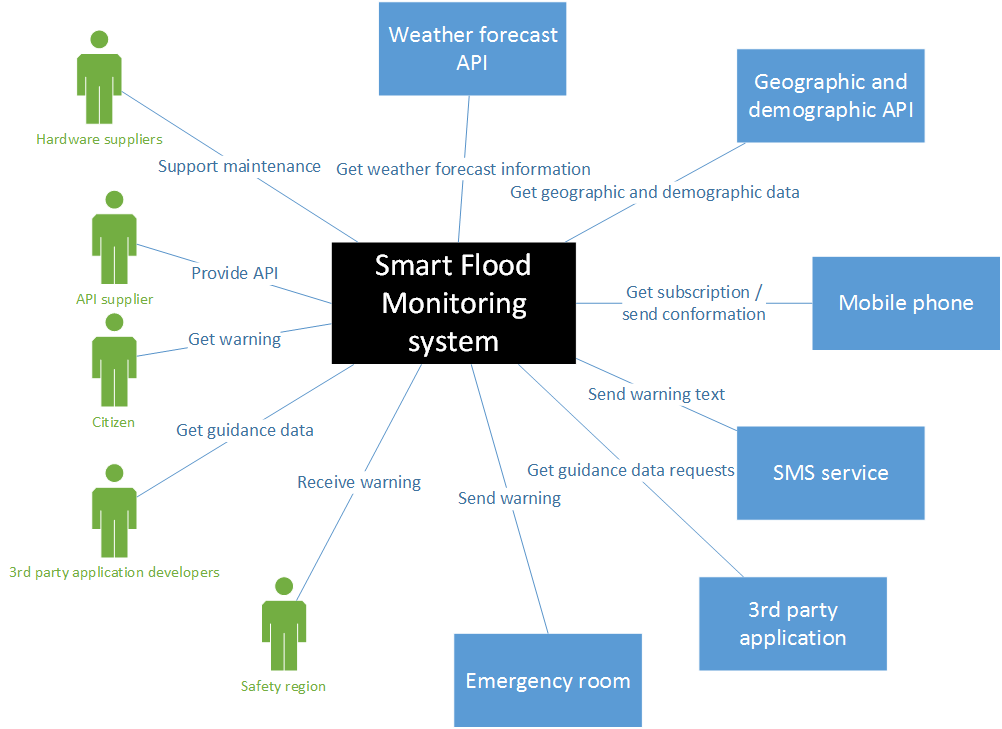
\includegraphics[keepaspectratio=true,width=0.7\textwidth]{images/system_context.png}
\caption{System context diagram}
\label{fig:system-context-diagram}
\end{figure}

\subsection{Users and Roles}
\begin{description}
	\item[Safety region] The safety region has the responsibility to protect citizens when a dangerous situation occurs, in this system floods. They receive a warning when there is a imminent flood. When the warning is received, the safety region can warn citizens and emergency services. The safety region needs information about time to evacuate, location , and severity of imminent flood.
	% \item[Citizens] Citizens can subscribe for receiving warnings in case of an imminent flood. Citizen will receive a warning when they are in an area which might get flooded. The warning consists of a message that they are in a dangerous area and should turn on TV or radio or surf to a safety region website in order to receive information how to protect yourself.
	\item[Third party application developers] This user will build an application to provide guidance when a flood is imminent. They use the data provided by the \gls{API} of the \gls{SFM}. They are allowed to get all relevant data from the system.
	\item[Hardware suppliers] This user will provide different kind of hardware to the system and repairs when hardware is failing
\end{description} 

\subsection{External Systems}
\begin{description}
	\item[Weather Forecast API] The system will utilize weather forecast services from third party sources. To make this input reliable, the system uses multiple weather forecast providers. To predict floods correctly the system will need: rain data, temperature data, tides data, air pressure data and wind data.
	\item[Geographic and demographic API] To predict how floods will evolve over time, we need geographical data. This data consists of maps of the area. There are multiple parameters that are needed by the system: ground height and waterways. To calculate the impact of an imminent flood on society, we also need to know how many people live in the affected area. This data is retrieved through the demographic API.
	% \item[Mobile phone] The mobile phone is a communication device of the citizen. This means a citizen uses the mobile phone to subscribe to the SMS service and to receive warnings in case of an imminent flood. This means the mobile phone should be able to send and receive text messages.
	\item[SMS service] The SMS system will communicate with the system and the mobile phones of the citizens. The SMS service keeps a list with all phone numbers that are subscribed to the service. When a warning is triggered by the central system, the SMS service gets a notification about this and sends the appropriate warning to the mobile phones that are within the area that is affected by the imminent flood.
	\item[Third party application] To guide citizens to a safe area in case of an imminent flood, we rely on third party applications. These applications get data from our API and deliver an app for citizens that provides guidance to a safe area.
	\item[Emergency room API] In case of an imminent flood we need to warn the safety region. This is done by invoking the emergency room API. In this way we send a message to the emergency room, which in their turn distributes this warning to the safety region.
\end{description}

\subsection{Channels and Information Flows}
\begin{table}[!htbp]
	\centering
    \begin{tabular}{L{\tw{0.2}} L{\tw{0.4}}}
    \toprule
    \multicolumn{2}{c}{$SFM\: \Leftrightarrow \: Weather \: forecast \: API$} \\ \midrule
    \textbf{Description} & The system gets rain, temperature, tides, airpressure and wind data. \\
    \textbf{Connection} & Wired, internet \\
    \textbf{Protocol} & TCP/IP \\
    \textbf{Transaction occurence} & Real time \\
    \bottomrule
    \end{tabular}
\end{table}

\begin{table}[!htbp]
	\centering
    \begin{tabular}{L{\tw{0.2}} L{\tw{0.4}}}
    \toprule
    \multicolumn{2}{c}{$SFM \: \Leftrightarrow \: Geographic \: and \: demographic \: API$} \\ \midrule
    \textbf{Description} & The system gets ground height data, waterway data and the amount of people who live in the affected area.\\
    \textbf{Connection} & Wired, internet \\
    \textbf{Protocol} & TCP/IP \\
    \textbf{Transaction occurence} & Real time \\
    \bottomrule
    \end{tabular}
\end{table}

% \begin{table}[!htbp]
% 	\centering
%     \begin{tabular}{L{\tw{0.2}} L{\tw{0.4}}}
%     \toprule
%     \multicolumn{2}{c}{$SFM \: \Leftrightarrow \: Mobile \: Phone$} \\ \midrule
%     \textbf{Description} & The mobile phone can subscribe to \\
%     \textbf{Connection} & Wireless, Internet \\
%     \textbf{Protocol} & 4G \\
%     \textbf{Transaction occurance} & Real time \\
%     \bottomrule
%     \end{tabular}
% \end{table}

\begin{table}[!htbp]
	\centering
    \begin{tabular}{L{\tw{0.2}} L{\tw{0.4}}}
    \toprule
    \multicolumn{2}{c}{$SFM \: \Leftrightarrow \: SMS \: Service$} \\ \midrule
    \textbf{Description} & The SMS service receives subscriptions and sends warning messages to the right phone numbers when it gets warned by the system. \\
    \textbf{Connection} & Wired, internet \\
    \textbf{Protocol} & TCP/IP \\
    \textbf{Transaction occurence} & In case of an imminent flood \\
    \bottomrule
    \end{tabular}
\end{table}

\begin{table}[!htbp]
	\centering
    \begin{tabular}{L{\tw{0.2}} L{\tw{0.4}}}
    \toprule
    \multicolumn{2}{c}{$SFM \: \Leftrightarrow \: Third \: party \: applications$} \\ \midrule
    \textbf{Description} & The system will provide data to the third party applications through the API.\\
    \textbf{Connection} & Wired, internet \\
    \textbf{Protocol} & TCP/IP \\
    \textbf{Transaction occurence} & Real time \\
    \bottomrule
    \end{tabular}
\end{table}

\begin{table}[!htbp]
	\centering
    \begin{tabular}{L{\tw{0.2}} L{\tw{0.4}}}
    \toprule
    \multicolumn{2}{c}{$SFM \: \Leftrightarrow \: Emergency \: room \: API$} \\ \midrule
    \textbf{Description} & The system warns the the safety region through the emergency room API. \\
    \textbf{Connection} & Wired, internet \\
    \textbf{Protocol} & TCP/IP \\
    \textbf{Transaction occurence} & In case of an imminent flood \\
    \bottomrule
    \end{tabular}
\end{table}


\subsection{Alternatives}
\subsubsection*{Geographic and demographic data}
The system will use an API to get the latest geographic and demographic data. It would also have been possible to download the data and import it just one time. However, the data needs to be up to date. This means the data needs to be updated once in a while, the easiest way to do this is by invoking an API.

\subsubsection*{SMS Service}
To warn the citizens in case of an imminent flood, we use an external SMS service. Citizens can subscribe to this service and receive a warning. Another option is that the system uses its own SMS service. The advantage of this is that we keep control of the process of warning citizens. However, it would be expensive to implement such a service. Besides this, outsourcing is more scalable since we don't have to cope with problems of sending text messages to other countries.

Another way of informing citizens would be to send a whatsapp message. However, all mobile phones are able to receive text messages, while not all mobile phones have internet access to receive whatsapp messages.  

\subsubsection*{Emergency room}
The emergency room will be warned by invoking their API. This decission was made to make sure all data will be received correctly. By warning the emergency room through telephone it would be possible the employee could accidently forget or change some of the information. If this would be implemented the SFM would need an employee 24/7, which is expensive. 

Another option would have been to send an email in case of an imminent flood. However, in this case it wouldn't be possible to continously update the information in the dashboard of the emergency service. This could also be achieved by continously sending mails, but this would take more time to open and interpret the emails.



%!TEX root = ../report.tex
\section{Elaborated Model}
\label{sec:elaboratedmodel}

In figure \ref{fig:system-context-diagram} the system architecture model is shown. This figure is an elaborated version of the system context figure in chapter 5.1. The arrows at the end of the lines represent data flows, going in that direction. 
First of all the system retrieves data from external API's. The data is retrieved by the data collection system and send to the database. The same applies for the UAV and sensor data. Besides this data flow, there is also a data flow from the data collection system to the UAV. In case the system detects that it needs UAV data, the data collection system sends commands to the UAV. The data collection system also retrieves the phone numbers and addresses of the citizens who have subscribed to the SMS service. After all data is collected the algorithm component will determine the flood probability based on the known data. If it detects that a flood is imminent, a warning message is sent to the warning system. This warning part then warns the emergency room by invoking the API. It also sends a text message to all the citizens that are in the affected area. To provide data to the third party applications the system holds an API. This API can be used by third party developers to get relevant data from the database. 
\begin{figure}[H]
	\centering
	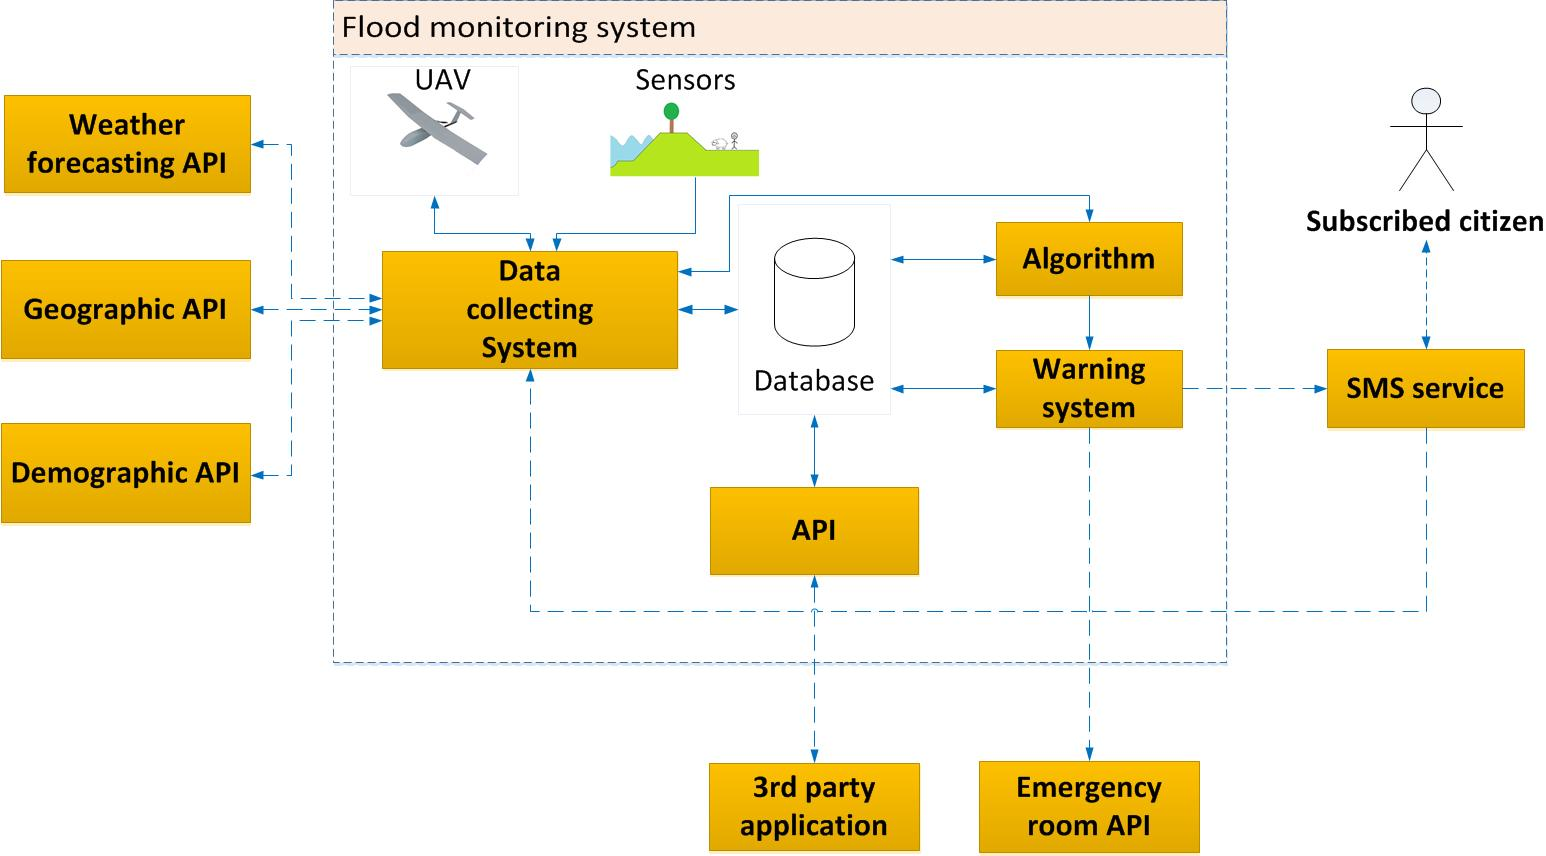
\includegraphics[keepaspectratio=true,width=1\textwidth]{images/Model_v3.jpg}
	\caption{Elaborated system context diagram}
	\label{fig:elaborated-model}
\end{figure}

%!TEX root = ../report.tex
\section{Verification}
The feasibility of the \ProjectName{} is verified in the following section.

\subsection{Reliability}
To determine the reliability of the system we determine the reliability of the separate components. Let:\\
MTBF: Mean Time Between Failure\\
MTTR: Mean Time To Repair \\
The reliability of the complete system is given as $x$\\
$x = {MTBF \over{MTBF + MTTR}}$

\subsection{Time to Market}
All external services already excist. 

\subsection{Cost}
Cost of API's we use for our system.


%!TEX root = ../report.tex
\chapter{Hardware Architecture}
\label{ch:hardware}
This section describes the hardware architecture of SFM. The description will be more high-level along with explanations about the hardware platform and the application interfaces between each components of the system. The rest of this chapter is organized as follows; First section, \autoref{sec:hardware-overview}, presents an overview of the hardware implemented in this system depicted in big schema. Decisions made in this system are detailed in \autoref{sec:hardware-decisions} with tables. Lastly, hardware description is described in \autoref{sec:hardware-description}.

\section{Hardware Overview}
\label{sec:hardware-overview}
The SFM hardware components can be categorized into four main components: sensing part, data storing part, analytics part, and data presentation part. The data flow starts from wired and wireless sensors located across the Netherlands that collects information for monitoring. The process will end at data presentation and warning dispatch in the users' side. The overview of the hardware and its application interfaces are depicted in \autoref{fig:hardware-archi-schema} below.

% btw is it suppose to be the other way around? sensor monitoring -> analytics-> database ?
%\begin{figure}[hb!]
%\centering
%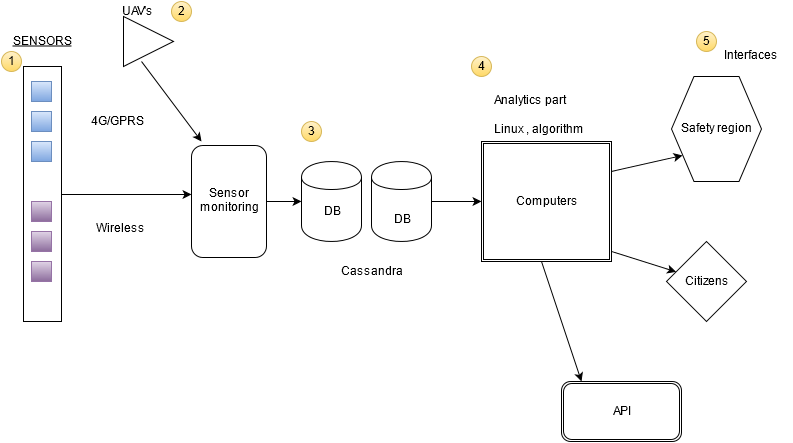
\includegraphics[scale=0.5]{images/HardwareArchitectureOverview.png}
%\caption{Schematic overview of the hardware architecture of \ProjectName{}}
%\label{fig:hardware-archi-schema}
%\end{figure}
\begin{figure}[hb!]
\centering
\includegraphics[scale=0.4]{6-hardware/images/hardwareoverview.png}
\caption{Schematic overview of the hardware architecture of \ProjectName{}}
\label{fig:hardware-archi-schema}
\end{figure}

Here is an overview of the Hardware Architecture. Each number corresponds to a decision which will be detailed in the Hardware Design Decision part.

The SFM will utilize wired and wireless sensor for monitoring water ways and dikes. Wired sensor will be placed in congested dikes and waterways where wired connection is possible. Wireless sensor will be planted in remote areas where wired connections are impossible or too costly. UAVs will fly to check reported faulty sensors. UAVs will also be used to take required pictures for further analytics or to examine some portion of the system which is hard or impossible for a personnel to access. Then all measurement will be forwarded to sensor monitoring part to be normalized before getting in to the analytics part.

The next part of the hardware is the cluster for carrying out analysis. This will be a collection of servers that is coordinated using clusters. This part also handles the logic for detecting faulty sensors, as the sensor monitoring parts contain no logic behind it.

SFM will use other cluster to store our important data. This cluster will run Cassandra database on top if it. This cluster will also have several interfaces to communicate with other instances, such as main analytics part, third party data gathering cluster, and API cluster.

The last part of the hardware architecture is third party data gathering cluster and API cluster. Third party data gathering cluster is responsible for collecting weather forecast and demographic information of the Netherlands. Meanwhile, API cluster is responsible for handling request from actors that will consume our practical information and for notifying safety region in case of imminent flood. Both of this cluster are merely collections of server computer that works together.

\section{Hardware Design Decisions}
\label{sec:hardware-decisions}
This section defines decisions made regarding the hardware selection. Tables will be used to make our justification in regard to hardware selection more crystal clear.

% ng180levee
\begin{table}[h!]
\begin{tabular}{L{0.2\textwidth} L{0.6\textwidth}}
    \textbf{Name}           & \textbf{Choice of dike sensor} \\ \toprule
    \textbf{Decision}       & \textbf{HW-\textbf{\nextNrRef{hw}}}\\ \midrule
    \textbf{Status}         & \textbf{Approved} \\ \midrule
    \textbf{Problem/Issue}  & The system needs a reliable sensor system to measure condition of dikes. \\ \midrule
    \textbf{Decision}       & The system will implement GeoBeads MEMS Sensor in dikes.\\ \midrule
    \textbf{Alternatives}   & \textit{GeoBeads}\\
                            & The GeoBead is a compact sensor, which can measure the pore pressure, temperature and local tilt in dikes. A unit costs about 350 dollar\cite{ng180levee}. \\
                            & \textit{Piezometers}\\
                            & Piezometers measure the pore water pressure in the dikes. This information can be used to measure the stability of the dike. A piezometer costs about 200 dollar\cite{ng180levee}. \\
                            & \textit{Volt meters} \\
                            & Volt meters can be used to measure the streaming potential in the dike, which are an indicator of its stability\cite{selfpotential}. These sensors are approximately 50 dollars per unit. Materials in the dike can decrease the accuracy of this measurement technique. \\
                            \midrule
    \textbf{Arguments}      & \\
                            &   \begin{tabular}{l|lllllll|l}
                            &       \rot{Reliability} & \rot{Resilience} & \rot{Performance}& \rot{Interoperability} & \rot{Security} & \rot{Scalability} & \rot{Cost} & \rot{\textbf{Score}} \\ \hline
                            %                  rel res perf int sec sca cost
                                    GeoBeads   & 5 & 4 &  & 3 &    &   & 2 & 14\\ 
                                    Piezometer & 4 & 2 &  & 2 &    &   & 3 & 11\\
                                    Volt meters& 1 & 5 &  & 2 &    &   & 5 & 13\\
                                \end{tabular} \\
    \\ \bottomrule
\end{tabular}
\caption{Decision -- Choice of Sensors}
\label{table:linux}
\end{table}


% ng180levee
\begin{table}[h!]
\begin{tabular}{L{0.2\textwidth} L{0.6\textwidth}}
    \textbf{Name}           & \textbf{Connectivity of the dike sensor} \\ \toprule
    \textbf{Decision}       & \textbf{HW-\textbf{\nextNrRef{hw}}}\\ \midrule
    \textbf{Status}         & \textbf{New} \\ \midrule
    \textbf{Problem/Issue}  & The dike sensors have to be connected to the internet in some way, so they can send their data to the central server. \\ \midrule
    \textbf{Decision}       & The sensors will be connected by a wire.\\ \midrule
    \textbf{Alternatives}   & \textit{Wired}\\
                            & A wired cable connects the dike sensor. This cable can also be used to supply the sensor with electricity. \\
                            & \textit{ZigBee}\\
                            & ZigBee is an open protocol for personal area networks. It uses little power and is therefore a good choice for devices equipped with a battery. \\
                            & \textit{ISM radio band} \\
                            & The ISM radio bands can be used for industrial, scientific and medical purposes.  \\
                            \midrule
    \textbf{Arguments}      & ZigBee is not an option, since the sensors are embedded in the soil of the dikes, and the frequency it uses, decreases too much in strength when traveling through the dike\cite{van2009draadloos}. \\
                            & Research has been done by van der Gees and Kok \cite{van2009draadloos} to determine if it is feasible to use the ISM radio band to communicate from within the dike. They concluded that, while it is possible to communicate through the dike using this band, the distance is limited and the rate of error is relatively high.
                            \\
                            & While a wire is not ideal in the sense that it will have to connect all the sensors, it seems to be the best option for the sensor in the dikes. It has the additional benefit that it can also supply the sensors with electricity.
    \\ \bottomrule
\end{tabular}
\caption{Decision -- Connectivity of the dike sensor}
\label{table:linux}
\end{table}

\begin{table}[h!]
\begin{tabular}{L{0.2\textwidth} L{0.6\textwidth}}
    \textbf{Name}           & \textbf{Analytic cluster selection} \\ \toprule
    \textbf{Decision}       & \textbf{HW-\textbf{\nextNrRef{hw}}}\\ \midrule
    \textbf{Status}         & \textbf{Approved} \\ \midrule
    \textbf{Problem/Issue}  & SFM needs a reliable computers to do the analytical processing. \\ \midrule
    \textbf{Decision}       & SFM will use clustered Dell PowerEdge R530 to act as the main analytic cluster and to provide API to the actors.\\ \midrule
    \textbf{Alternatives}   & \textit{HP ProLiant DL360 Gen9 Base}\\
                            % https://www.google.nl/shopping/product/12299869794181781707?biw=1346&bih=669&q=servers&bav=on.2,or.r_cp.&bvm=bv.104317490,d.d2s&ion=1&espv=2&tch=1&ech=1&psi=1FIQVpOAEoPlaK7Zn4AN.1443910356406.15#sgro=om
                            & This server rack has 16GB of memory and 2.4GHz of processor speed. As other server computer, this machine utilizes Intel Xeon E5 2600v3. This server is suitable for high dense computing, however the price is not so suitable for this kind of specification. It does not have LCD screen that will help technician to look the current status of the server.\\
                            & \textit{Lenovo System x3550 M4 7914}\\
                            % https://www.google.nl/shopping/product/8704926690761174474?q=servers&biw=1346&bih=669&bav=on.2,or.r_cp.&bvm=bv.104317490,d.d2s&ion=1&espv=2&tch=1&ech=1&psi=1FIQVpOAEoPlaK7Zn4AN.1443910356406.17
                            & This server rack has only 8GB of memory. However, the processor is a bit faster, it runs on 2.6GHz. As other server computer, this machine also utilizes Intel XEON E5-2600. The price is a little bit lower than the others but the memory limitation makes it not so valuable. It has LCD screen that will help technician to look the current status of the server. \\
                            & \textit{Dell PowerEdge R530} \\
                            % https://azerty.nl/0-3031-817940/dell-poweredge-r530-server-rack-uitvoering-2u-2-weg-1-x-xeon-e5-2620v3-2-4-ghz-ram-16-gb-sas-hot-swap-verwiss.html?channel_code=544&s2m_campaign=1CENT&s2m_product_id=817940
                            & This 2U server rack has 16GB of memory and 2.4GHz of processor speed. This machine utilizes Intel Xeon E5-2620V3 with 15MB of cache. This server is suitable for high dense computing. It has LCD screen that will help technician to look the current status of the server. \\
                            \midrule
    \textbf{Arguments}      & \\
                            &   \begin{tabular}{l|llllll|l}
                            &       \rot{Reliability} & \rot{Performance}& \rot{Interoperability} & \rot{Security} & \rot{Scalability} & \rot{Cost} & \rot{\textbf{Score}} \\ \hline
                            %                                       rel perf int sec sca cost
                                    Dell PowerEdge R530             & 5 & 5 & 4 & 4 & 4 & 5 & 27 \\ 
                                    Lenovo System x3550 M4 7914     & 4 & 4 & 4 & 3 & 4 & 4 & 23 \\
                                    HP ProLiant DL360 Gen9 Base     & 5 & 5 & 4 & 3 & 4 & 3 & 24 \\
                                \end{tabular} \\
    \\ \bottomrule
\end{tabular}
\caption{Decision -- Analytic cluster selection}
\label{table:server-selection}
\end{table}

\begin{table}[h!]
\begin{tabular}{L{0.2\textwidth} L{0.6\textwidth}}
    \textbf{Name}           & \textbf{Database cluster selection} \\ \toprule
    \textbf{Decision}       & \textbf{HW-\textbf{\nextNrRef{hw}}}\\ \midrule
    \textbf{Status}         & \textbf{Approved} \\ \midrule
    \textbf{Problem/Issue}  & The system needs reliable computers to store the data. \\ \midrule
    \textbf{Decision}       & SFM will utilize Synology RackStation RS814RP to store the data.\\ \midrule
    \textbf{Alternatives}   & \textit{Synology RackStation RS814RP}\\
                            % https://www.google.nl/shopping/product/9793555443596138172?biw=1346&bih=669&q=storage+servers&bav=on.2,or.r_cp.&bvm=bv.104317490,d.d2s&ion=1&espv=2&tch=1&ech=1&psi=1FIQVpOAEoPlaK7Zn4AN.1443910356406.23&prds=paur:ClkAsKraX8aViW9QBHq_YeLbadvaW6lnMVQDuwzotG6gRVknHILZ_EDzrO8nQNS6N477UjRspRo17BmUoyZnQjMDnOrhflRLM5VXFQCOPDxn9wCZnGJxrWXfWxIZAFPVH73DWMclCanKIzQ68mJVd6ADLpvTfg&sa=X&ved=0CMkDEM1KMBJqFQoTCLid3qaqp8gCFYrZGgodX70Kow
                            & This storage machine has the fastest connection among the others. This machine will run at SATA with 6 Gbps connection.\\
                            & \textit{70BJ NAS-server}\\
                            % https://www.google.nl/shopping/product/15463250681911940369?q=storage+servers&biw=1346&bih=669&bav=on.2,or.r_cp.&bvm=bv.104317490,d.d2s&ion=1&espv=2&tch=1&ech=1&psi=1FIQVpOAEoPlaK7Zn4AN.1443910356406.25&prds=paur:ClkAsKraXy1_BVqi5aD5CGi7OmupTi3OwyL-j7nW7Ss2Qwo-W_81sjaidQU8J0Q3uu7RrSCCth3c9YuMEMNA3zO6TM9tfutSn6ksUeo1EGFdUDKUIlB4gt8wBBIZAFPVH70byN_Dqe5qhSCABb7sxVXYXAvfaw&sa=X&ved=0CIEDEM1KMAo4FGoVChMIpJb_tKqnyAIVQUwaCh0d6wGT
                            & This machine form factor is 1U which is suitable for saving space. However, the connection speed is limited to 3 Gbps.\\
                            & \textit{Thecus N8810U-G NAS-server} \\
                            % https://www.google.nl/shopping/product/464537487289413504?q=storage+servers&biw=1346&bih=669&bav=on.2,or.r_cp.&bvm=bv.104317490,d.d2s&ion=1&espv=2&tch=1&ech=1&psi=1FIQVpOAEoPlaK7Zn4AN.1443910356406.25&prds=paur:ClkAsKraXylXtQJRG2pDp_XW-OBbRHsXe6nrmcB3olgeJQi1FhG4T8bXQABWVbkevi6hzBMwfTk7qioWd88Cq3GWIt3hQlEi5oJEmR7vZvXtvtEinYYlhn3_bBIZAFPVH71qflxmS1BuYghV4B5tpcohhFU7vQ&sa=X&ved=0CNQCEM1KMAU4FGoVChMIpJb_tKqnyAIVQUwaCh0d6wGT
                            & This machine also runs in 3Gbps connection. However, the form factor is 2U which makes this machine takes more space in the rack.\\
                            \midrule
    \textbf{Arguments}      & \\
                            &   \begin{tabular}{l|llllll|l}
                            &       \rot{Reliability} & \rot{Performance}& \rot{Interoperability} & \rot{Security} & \rot{Scalability} & \rot{Cost} & \rot{\textbf{Score}} \\ \hline
                            %                                       rel perf int sec sca cost
                            Synology RackStation RS814RP    & 5 & 4 & 4 & 4 & 4 & 4 & 25 \\ 
                            70BJ NAS-server                 & 4 & 3 & 4 & 4 & 4 & 3 & 22 \\
                            Thecus N8810U-G NAS-server      & 4 & 3 & 4 & 4 & 4 & 3 & 22 \\
                                \end{tabular} \\
    \\ \bottomrule
\end{tabular}
\caption{Decision -- Choice of storage machine.}
\label{table:database-selection}
\end{table}

\begin{table}[h!]
\begin{tabular}{L{0.2\textwidth} L{0.6\textwidth}}
    \textbf{Name}           & \textbf{High Performance Switch selection} \\ \toprule
    \textbf{Decision}       & \textbf{HW-\textbf{\nextNrRef{hw}}}\\ \midrule
    \textbf{Status}         & \textbf{Approved} \\ \midrule
    \textbf{Problem/Issue}  & SFM cluster needs a powerful high performance switch to connect each cluster. \\ \midrule
    \textbf{Decision}       & SFM will use Cisco Catalyst 2960S-24TS-L Switch.\\ \midrule
    \textbf{Alternatives}   & \textit{Linksys LGS552P Switch}\\
                            % https://www.google.nl/shopping/product/15955701749855379542?biw=1346&bih=669&q=network+switch&sqi=2&bav=on.2,or.r_cp.&bvm=bv.104317490,d.d2s&ion=1&espv=2&tch=1&ech=1&psi=1FIQVpOAEoPlaK7Zn4AN.1443910356406.33&prds=paur:ClkAsKraX5ryPFpohZJ3cHRR5Y04pVrqqvR-5nXru2N7X2-97H3V7DAZtCjwWh2BPthulxNJ2ahSWe7PR9qBPpG4AcckL_q3UHXeyd1fqIcsRCo9aEhM_4ihYhIZAFPVH7186CU9loBEx5Tx9iwfjvLu2xB6eg&sa=X&ved=0CM4CEM1KMAJqFQoTCJaXr-ahqMgCFUh-Ggodym4G5w
                            & This switch has 52 ports available for connection, which is very good for scalability. However the performance is not as good as Cisco catalyst switch series.\\
                            & \textit{HP 1820-48G Switch}\\
                            % https://www.google.nl/shopping/product/7539423950361123669?biw=1346&bih=669&q=network+switch&sqi=2&bav=on.2,or.r_cp.&bvm=bv.104317490,d.d2s&ion=1&espv=2&tch=1&ech=1&psi=1FIQVpOAEoPlaK7Zn4AN.1443910356406.33&prds=paur:ClkAsKraX2rp4gF8ATRwWJuY5iaZuchaa1sdhIz6lvepgxugqRb5mZxy8yAXts_70QyVg33fwd3C8WiFm3ThxDkZDi6gz2-ogcVLZ1Frs8QHH9IhEd-rj9s-CBIZAFPVH71WuYA_yyIRCl_FpDi93AJr9DX5QQ&sa=X&ved=0CNgCEM1KMANqFQoTCJaXr-ahqMgCFUh-Ggodym4G5w
                            & This switch has lesser available ports than Linksys switch. It has 48 ports available. This switch is not very configurable which makes this not so suitable for high performance switching. \\
                            & \textit{Cisco Catalyst 2960S-24TS-L Switch} \\
                            % https://www.google.nl/shopping/product/3278668597556943908?biw=1346&bih=669&q=network+switch&sqi=2&bav=on.2,or.r_cp.&bvm=bv.104317490,d.d2s&ion=1&espv=2&tch=1&ech=1&psi=1FIQVpOAEoPlaK7Zn4AN.1443910356406.33&prds=paur:ClkAsKraXw_7YyEqvAKzRJjfEM3yN-4kzC4NaE-smcis8WFMegcToXlCuBmXRPb647qqqZU34GfFxp8EYHh7FC1AVCwaCRNTWcvFYI4Ppe8B8xT_2AMPJ7r3XBIZAFPVH72nlGbb8LwIOpZWGX8ZHfTvUUmDSw&sa=X&ved=0CPUCEM1KMAZqFQoTCJaXr-ahqMgCFUh-Ggodym4G5w
                            & This switch has the lowest number of port available, 24 ports. However, Cisco Catalyst is very configurable and has a very good security. \\
                            \midrule
    \textbf{Arguments}      & \\
                            &   \begin{tabular}{l|llllll|l}
                            &       \rot{Reliability} & \rot{Performance}& \rot{Interoperability} & \rot{Security} & \rot{Scalability} & \rot{Cost} & \rot{\textbf{Score}} \\ \hline
                            %                                   rel perf int sec sca cost
                            Cisco Catalyst 2960S-24TS-L Switch  & 5 & 5 & 4 & 5 & 3 & 4 & 26 \\ 
                            Linksys LGS552P Switch              & 4 & 4 & 4 & 3 & 4 & 5 & 24 \\
                            HP 1820-48G Switch                  & 3 & 4 & 4 & 3 & 4 & 5 & 23 \\
                                \end{tabular} \\
    \\ \bottomrule
\end{tabular}
\caption{Decision -- Choice of high performance switch}
\label{table:switch-selection}
\end{table}


\clearpage
\section{Hardware Description}
\label{sec:hardware-description}
% Mention the difference between previous chapter
This section gives an outline of the hardware implemented in this system. This section also elaborates on hardware decisions.

\subsection{Sensor Components}
\label{subsec:sensing-components}
Roughly 17.000 kilometers of dikes protect the Netherlands against flooding\cite{DMC}. Of this, about 3.500 kilometers are primary dikes\cite{waterwijzer}. These are dikes protecting against the water of the sea, the big rivers (Rijn, Maas, IJssel), the IJsselmeer and the Markermeer. 

The hardware architecture of the system is composed of two sensor components. The first sensor component are sensors installed in the dikes to measure and detect potential instability of the dikes.
The second sensing component consists of water level sensors, which are spread along water ways in the country, to measure the water level. 

\label{dikesensors}
\subsubsection{Dike sensors}
To measure the stability of the dikes, the GeoBeads dike monitoring sensor will be installed in the dikes. When these sensors are placed in the dike with a spacing of 3 meters, they will provide optimal measurements\cite{ng180levee}. The GeoBead will measure the water pressure, temperature, inclination and acceleration.

A GeoBead sensor consists of several modules, loosely connected by cable, which form a chain of sensors. The GeoBeads will be installed in a pre-drilled vertical hole, or where this is not possible, horizontally. Three sensors are installed per cross-section and a cross-section is installed every 100 m. 

The GeoBeads are connected by communication cable, which also functions as a power supply. 

\subsubsection{Water level sensors}
The water level sensors are placed next to the dikes and in the water ways. A water level sensor is placed every 300 meters. % WM: why 300 meters, elaborate.

The water levels sensors are accommodated with a connectivity chip, which allows it to use the mobile broadband to connect to the central server.
% TODO: decide on exact water level sensor
% is it feasible to use a battery for water pressure sensor?


\subsection{Database Cluster and Data Collection}
\label{subsec:database-data}
In the previous chapter, SFM will use Cassandra database as the database platform. However, Cassandra requires computers to run its environment. SFM will use clusters of computer to manage database system and to store our data. The cluster will also be accessible by other portions of our hardware, such as main analytics parts and AAnPI part. The logical schematic of the database cluster is depicted in \autoref{fig:database-cluster}

\begin{figure}[hb!]
\centering
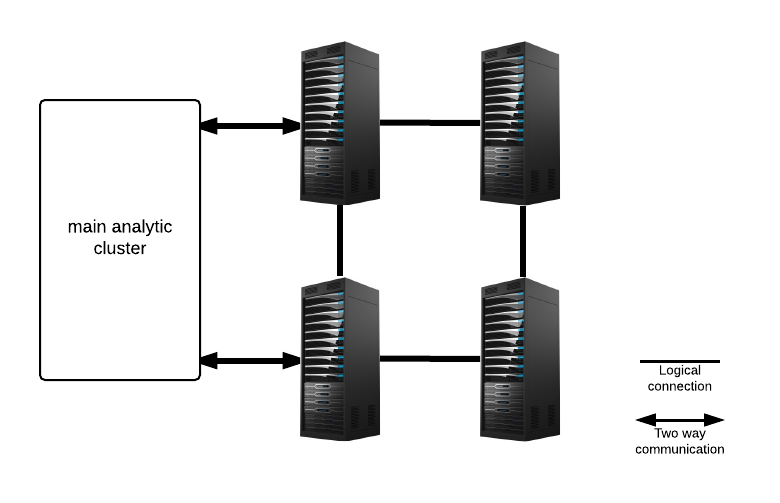
\includegraphics[]{6-hardware/images/db-cluster.png}
\caption{Logical schematic of database cluster of SFM}
\label{fig:database-cluster}
\end{figure}

As can be seen in \autoref{fig:database-cluster}, SFM will use four database racks to increase the reliability of the system. Using this kind of architecture, SFM will be more fault tolerant. There will also be two physical connection to the main analytic cluster to make this system more fault tolerant in terms of connection. SFM database cluster will use the same server, Dell PowerEdge R530, for controlling the SATA storage machine.

% Clustering, in the context of databases, refers to the ability of several servers or instances to connect to a single database. An instance is the collection of memory and processes that interacts with a database, which is the set of physical files that actually store data.

% Clustering offers two major advantages, especially in high-volume database environments:

% Fault tolerance: Because there is more than one server or instance for users to connect to, clustering offers an alternative, in the event of individual server failure.
% Load balancing: The clustering feature is usually set up to allow users to be automatically allocated to the server with the least load.

% Adds some picture here

\subsection{Analytics Components}
\label{subsec:analytics}
Analytics component will be the main brain of SFM. The intelligent algorithm will run on this machine. This components are also responsible for checking faulty sensors by analyzing incoming sensor data. Thus, there is a big dependency to this components. To increase availability and reliability, SFM will have six server racks to do the processing as depicted in \autoref{fig:analytic-cluster}.

\begin{figure}[hb!]
\centering
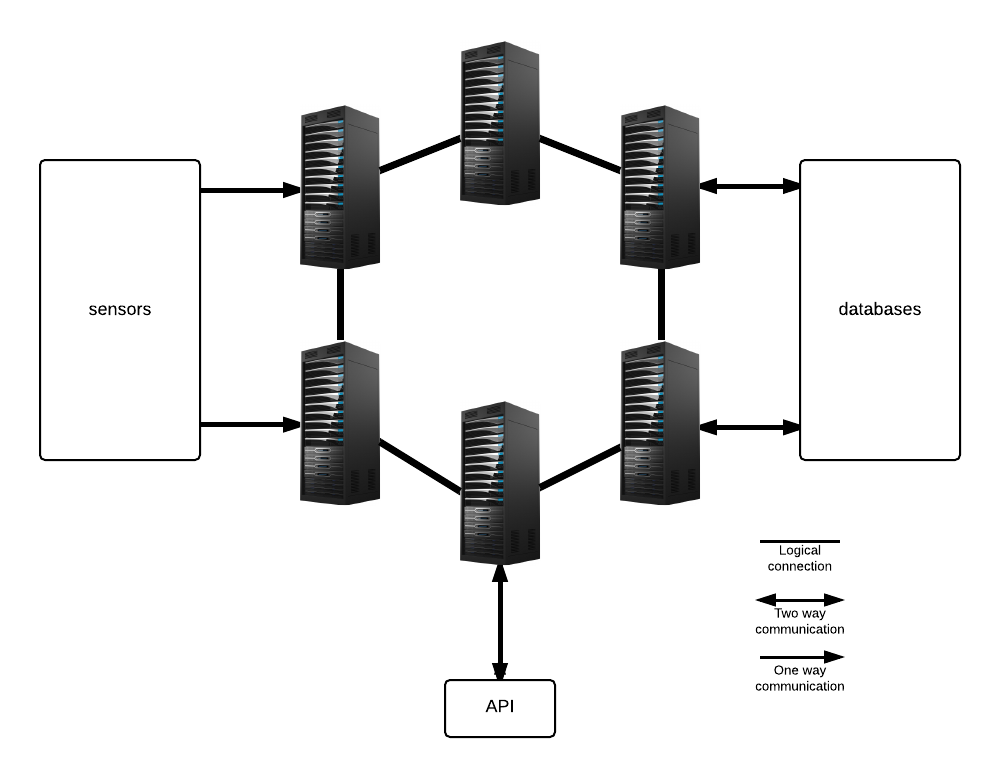
\includegraphics[]{6-hardware/images/analytic-cluster.png}
\caption{Logical schematic of analytic cluster of SFM}
\label{fig:analytic-cluster}
\end{figure}

The analytics components will also be the hub for the main connection of SFM. Thus, this system also need a high performance switch to accomplish this purpose. As have been mentioned before, this system will use Cisco Catalyst 2960S-24TS-L Switch.

The analytics components will use Dell PowerEdge R530 as server and it will be mounted on a server rack. The detailed hardware specifications of Dell PowerEdge R530 is listed in \autoref{table:server-specs}.

\begin{table}[!htbp]
    \centering
    \begin{tabular}{L{\tw{0.2}} L{\tw{0.4}}}
    \toprule
    \multicolumn{2}{c}{Dell PowerEdge R530 Specification} \\ \midrule
    \textbf{Item Description} & Dell PowerEdge R530 - E5-2620V3 Xeon 2.4 GHz - 16 GB - 1 TB \\
    \textbf{Type} & Server - rack-mountable \\
    \textbf{Height (Rack Units)} & 2U \\
    \textbf{Processor} & 1 x Intel Xeon E5-2620V3 / 2.4 GHz (3.2 GHz) (6-core) \\
    \textbf{Processor Main Features} & Intel Turbo Boost Technology 2 \\
    \textbf{Cache Memory} & 15 MB \\
    \textbf{Cache per processor} & 15 MB \\
    \textbf{RAM} & 16 GB (installed) / 384 GB (max.) - DDR4 SDRAM - 2133 MHz \\
    \textbf{Storage Controller} & RAID (SATA 6Gb / s) (Dell PERC H330) \\
    \textbf{Optical Storage} & DVD burner \\
    \textbf{Graphics Controller} & Matrox G200 \\
    \textbf{Video Memory} & 16 MB \\
    \textbf{Network} & GigE \\
    \textbf{Dimensions} &  (WxDxH)48.24 cm x 64.6 cm x 8.68 cm \\
    \textbf{Weight} & 2.14 kg \\
    \bottomrule
    \end{tabular}
\caption{Hardware specification of Dell PowerEdge R530}
\label{table:server-specs}
\end{table}


% Server specs
% - Server
% - Networking device
% - UPS

%!TEX root = ../report.tex
\chapter{Software Architecture}
\label{ch:software}
This chapter describes the software architecture of the SFM. This will be described in these four sections: software architecture design (attribute-driven design), architectural view, components, and software design decision.

%!TEX root = ../report.tex
\section{Software architecture design}
This section states software architecture design of the system with attribute-driven design method. As mentioned in \cite{smi-cme}, the Attribute-Driven Design (ADD) method is a systematic step-by-step method for designing the software architecture of a software-intensive system. It is an approach to defining software architectures by basing the design process on the architecture's quality attribute requirements. It follows a recursive decomposition process where, at each stage in the decomposition, tactics and architectural patterns are chosen to satisfy a set of quality attribute scenarios.

%!TEX root = ../report.tex
\section{Architectural view}
The following section will elaborate the views of the system into 4+1 Model: logical view, implementation view, process view, and deployment view.

\newcommand{\copied}[2]{}%\textcolor{red}{#1}\\\textcolor{green}{#2}}
\newcommand{\viewimages}{7-software/views/diagrams/}

%!TEX root = ../../report.tex
\subsection{Scenarios}
\copied{Scenarios : The description of an architecture is illustrated using a small set of use cases, or scenarios which become a fifth view. The scenarios describe sequences of interactions between objects, and between processes. They are used to identify architectural elements and to illustrate and validate the architecture design. They also serve as a starting point for tests of an architecture prototype. This view is also known as use case view.\\
	\\
	Scenarios are putting it all together. Interaction between objects in the
	system is expressed by object interaction and scenario diagrams as shown on
	Figure 6.
}
{from wikipedia\\\url{https://en.wikipedia.org/wiki/4\%2B1_architectural_view_model} and \url{http://pld.ttu.ee/~kruus/db_is02.pdf}}

This section describes the scenarios that are most likely to happen in our system. Scenarios are the interactions from our system with the different actors. First a textual step by step scenario is given, after that a diagram is shown with the scenario diagram.

\subsubsection*{Flood scenario}
\begin{enumerate}
  	\item The sensors monitor the water level
  	\item The algorithm requests weather forecast data
  	\item The weather forecast API returns the requested data
  	\item The algorithm sends a request to the UAV to validate results or provide extra images
  	\item The UAV provides the requested validation or extra images
  	\item The algorithm sends a warning to the warning part
  	\item The warning part requests the phone numbers from all subscribed citizens in the affected area
  	\item The database returns a list containing the corresponding phone numbers
  	\item The warning part invokes the emergency room API
  	\item The warning part invokes the SMS API, which sends a SMS to all phonenumbers on the list
\end{enumerate}

The different steps that are taken in the flood scenario are also represented in figure \ref{fig:flood-scenario}. This figure represents the logical connections that are made when a scenario is executed. This means that in reality a connection that is shown in the figure may not be made directly in reality. For example, the sensor data doesn't go directly from the sensors to the algorithm, there are some steps in between. 

\begin{figure}[H]
	%\centering
	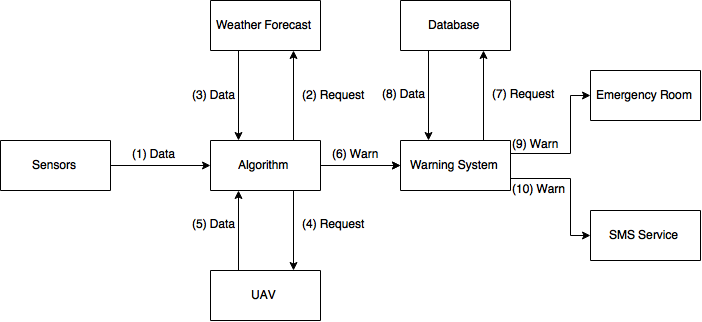
\includegraphics[keepaspectratio=true,width=0.9\textwidth]{{\viewimages/scenario1}.png}
	\caption{Scenario for a flood}
	\label{fig:flood-scenario}
\end{figure}

\subsubsection*{Guidance scenario}
\begin{enumerate}
	\item A citizen receives a warning text message
	\item A citizen requests guidance from a third party application to reach a safe area
	\item The third party application requests the current flood information from the third party API
	\item The third party API returns the requested data
	\item The third party application returns a route to a safe area
\end{enumerate}

When a flood is imminent or happening, a citizen can decide to request guidance to a safe area. If a citizen is subscribed to the SMS service, the citizen will get a warning text message in case of an imminent flood. Then the citizen can use a third party application that provides routes to safety that are as safe as possible.

\begin{figure}[H]
	%\centering
	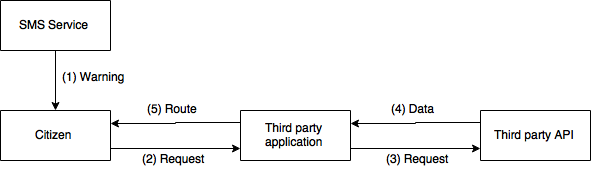
\includegraphics[keepaspectratio=true,width=0.9\textwidth]{{\viewimages/scenario2}.png}
	\caption{Scenario for guidance}
	\label{fig:guidance-scenario}
\end{figure}


%!TEX root = ../../report.tex
\subsection{Logical View}
\label{subsec:logicalview}

\copied{Logical view : The logical view is concerned with the functionality that the system provides to end-users. UML Diagrams used to represent the logical view include Class diagram, Communication diagram, Sequence diagram.[2]}
{from wikipedia\\\url{https://en.wikipedia.org/wiki/4\%2B1_architectural_view_model}}

The logical view shows the structural elements, key abstractions and mechanisms that are needed to realize the SFM. First an overview of the different components is provided. After that the components are decomposed and more details of the different layers are provided.

% This view shows the structural elements, key abstractions and mechanisms that are used within SFM to realize the systemics functionality. At first an overview of the components is provided. After that the main components are decomposed and desired in term of responsibilities and interfaces. In the end, the variability guide mentions parts of the software, which clarification is deferred until development/design phase.



%Used algorithms?:
%	hidden markov model with k means (unsupervised learning)
%	Singular Spectrum Analysis (SSA) for locations with tides?
%	“limit checking”
%	
%	Gauss-Markov
%	Something with correlation? https://en.wikipedia.org/wiki/Cross-correlation? Thesis zecht te kijken naar:
%	[74] Logan, D., Mathew, J. Using the Correlation Dimension for Vibration Fault
%Diagnosis of Rolling Element Bearing – I. Basic Concepts, Mechanical Systems and
%Signal Processing, Vol. 10, No. 3, pp. 241-250, (1996)
%[75] Logan, D., Mathew, J. Using the Correlation Dimension for Vibration Fault
%Diagnosis of Rolling Element Bearing – II. Selection of Experimental Parameters,
%Mechanical Systems and Signal Processing, Vol. 10, No. 3, pp. 251-264, (1996)

\subsubsection*{Layer pattern}
The software architecture of SMF is separated into three different layers. This layering is done according to the layering Martin Fowler proposes for enterprise applications \cite{Fowler:2002:PEA:579257,Fowler:web:servicelayer}.
Layering the software provides a more flexible architecture that allows modifications of layers having to alter the other layers.\\
The different software layers of SMF are listed below. Each of these layers will be discussed in more detail after the figure.

\begin{description}
	\item \textbf{Service layer} This layer provides services to external systems and coordinates the incomming calls to the domain layer.
	\item \textbf{Domain layer} The domain layer holds the core components for processing data and warning users.
	\item \textbf{Data source layer} This layer stores all relevant data that is needed or produced by the system. 
\end{description}

\clearpage
\begin{figure}[H]
	%\centering
	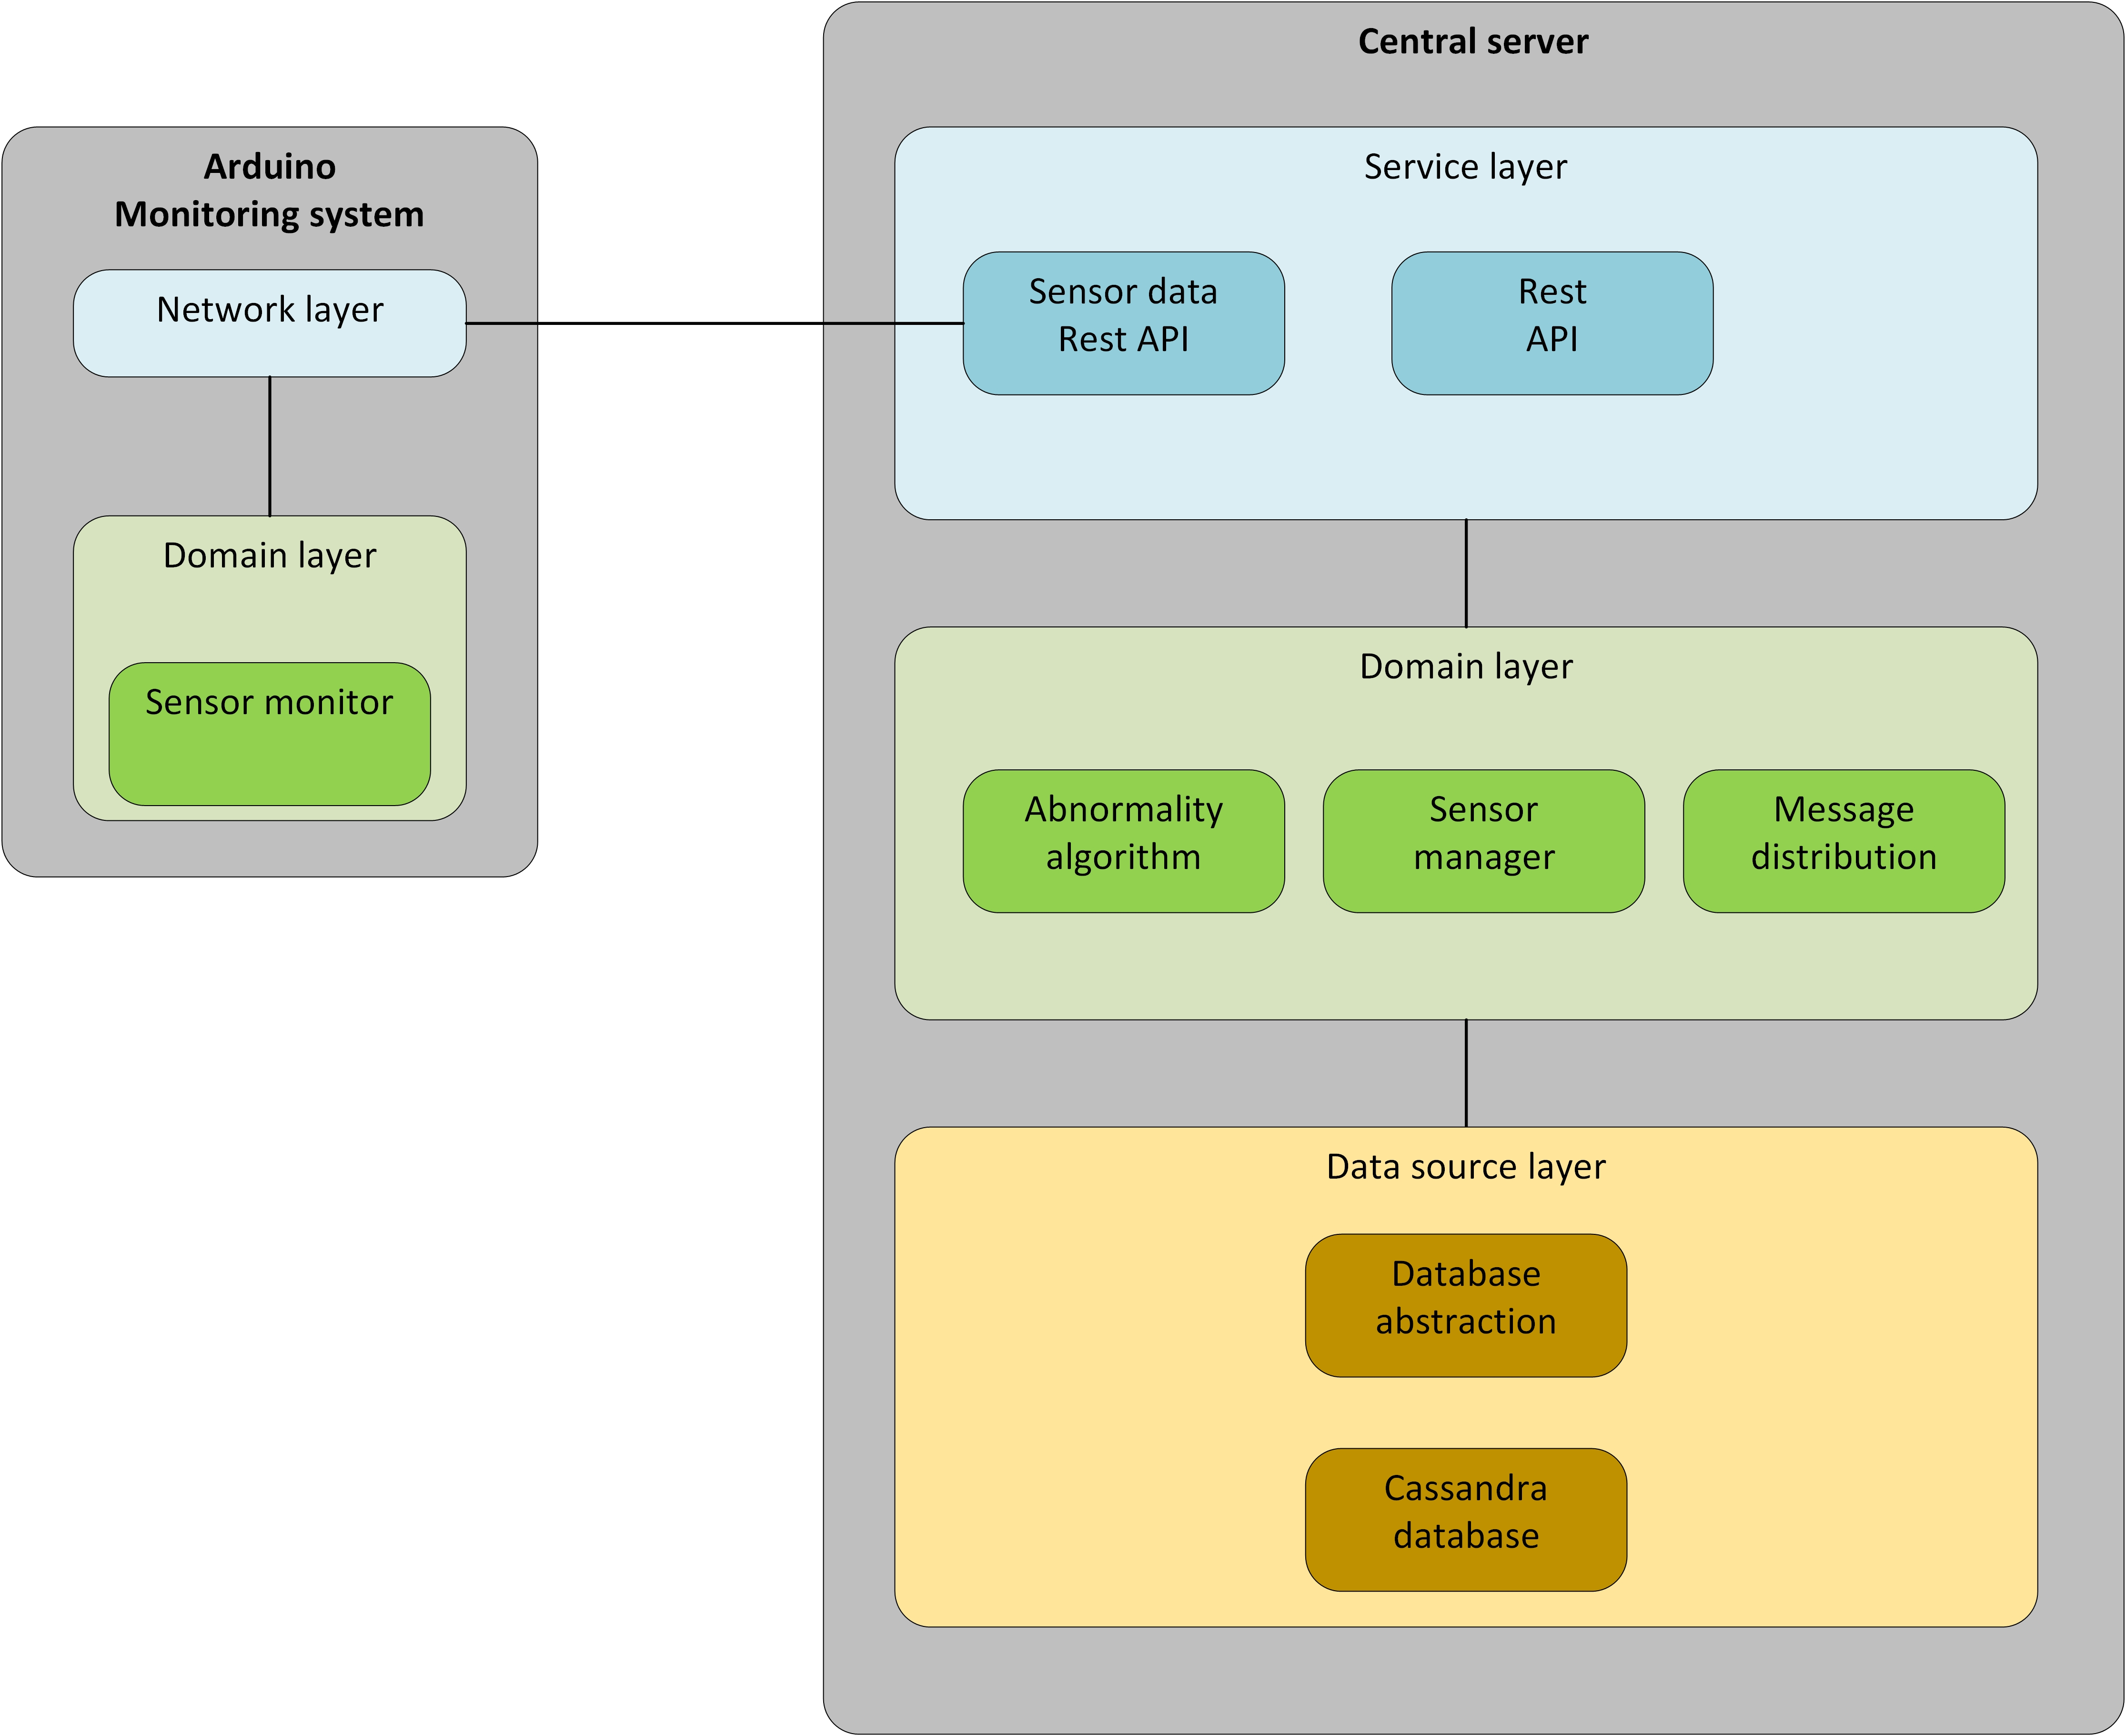
\includegraphics[keepaspectratio=true,width=0.9\textwidth]{{\viewimages/layers}.jpg}
	\caption{Layers of the software}
	\label{fig:layers}
\end{figure}

\subsubsection*{Service layer}
The Service layer pattern \cite{Fowler:2002:PEA:579257} is used as domain logic pattern. In this pattern, the service layer provides a set of operations that can be executed in the application. The service layer serves and coordinates the calls to these provides operation. The application logic in the domain layer is then separated from how it is called and how it should respond.\\
The main functionality of this layer consists of:
\begin{itemize}
	\item Providing a REST server the Arduino monitoring units can send their raw sensor data to
	\item Providing a REST server the third parties can use to receive flood data
	\item Distribute warning messages
\end{itemize}

The class diagram for this layer is shown in figure \ref{fig:service1}

\begin{figure}[H]
	\centering
	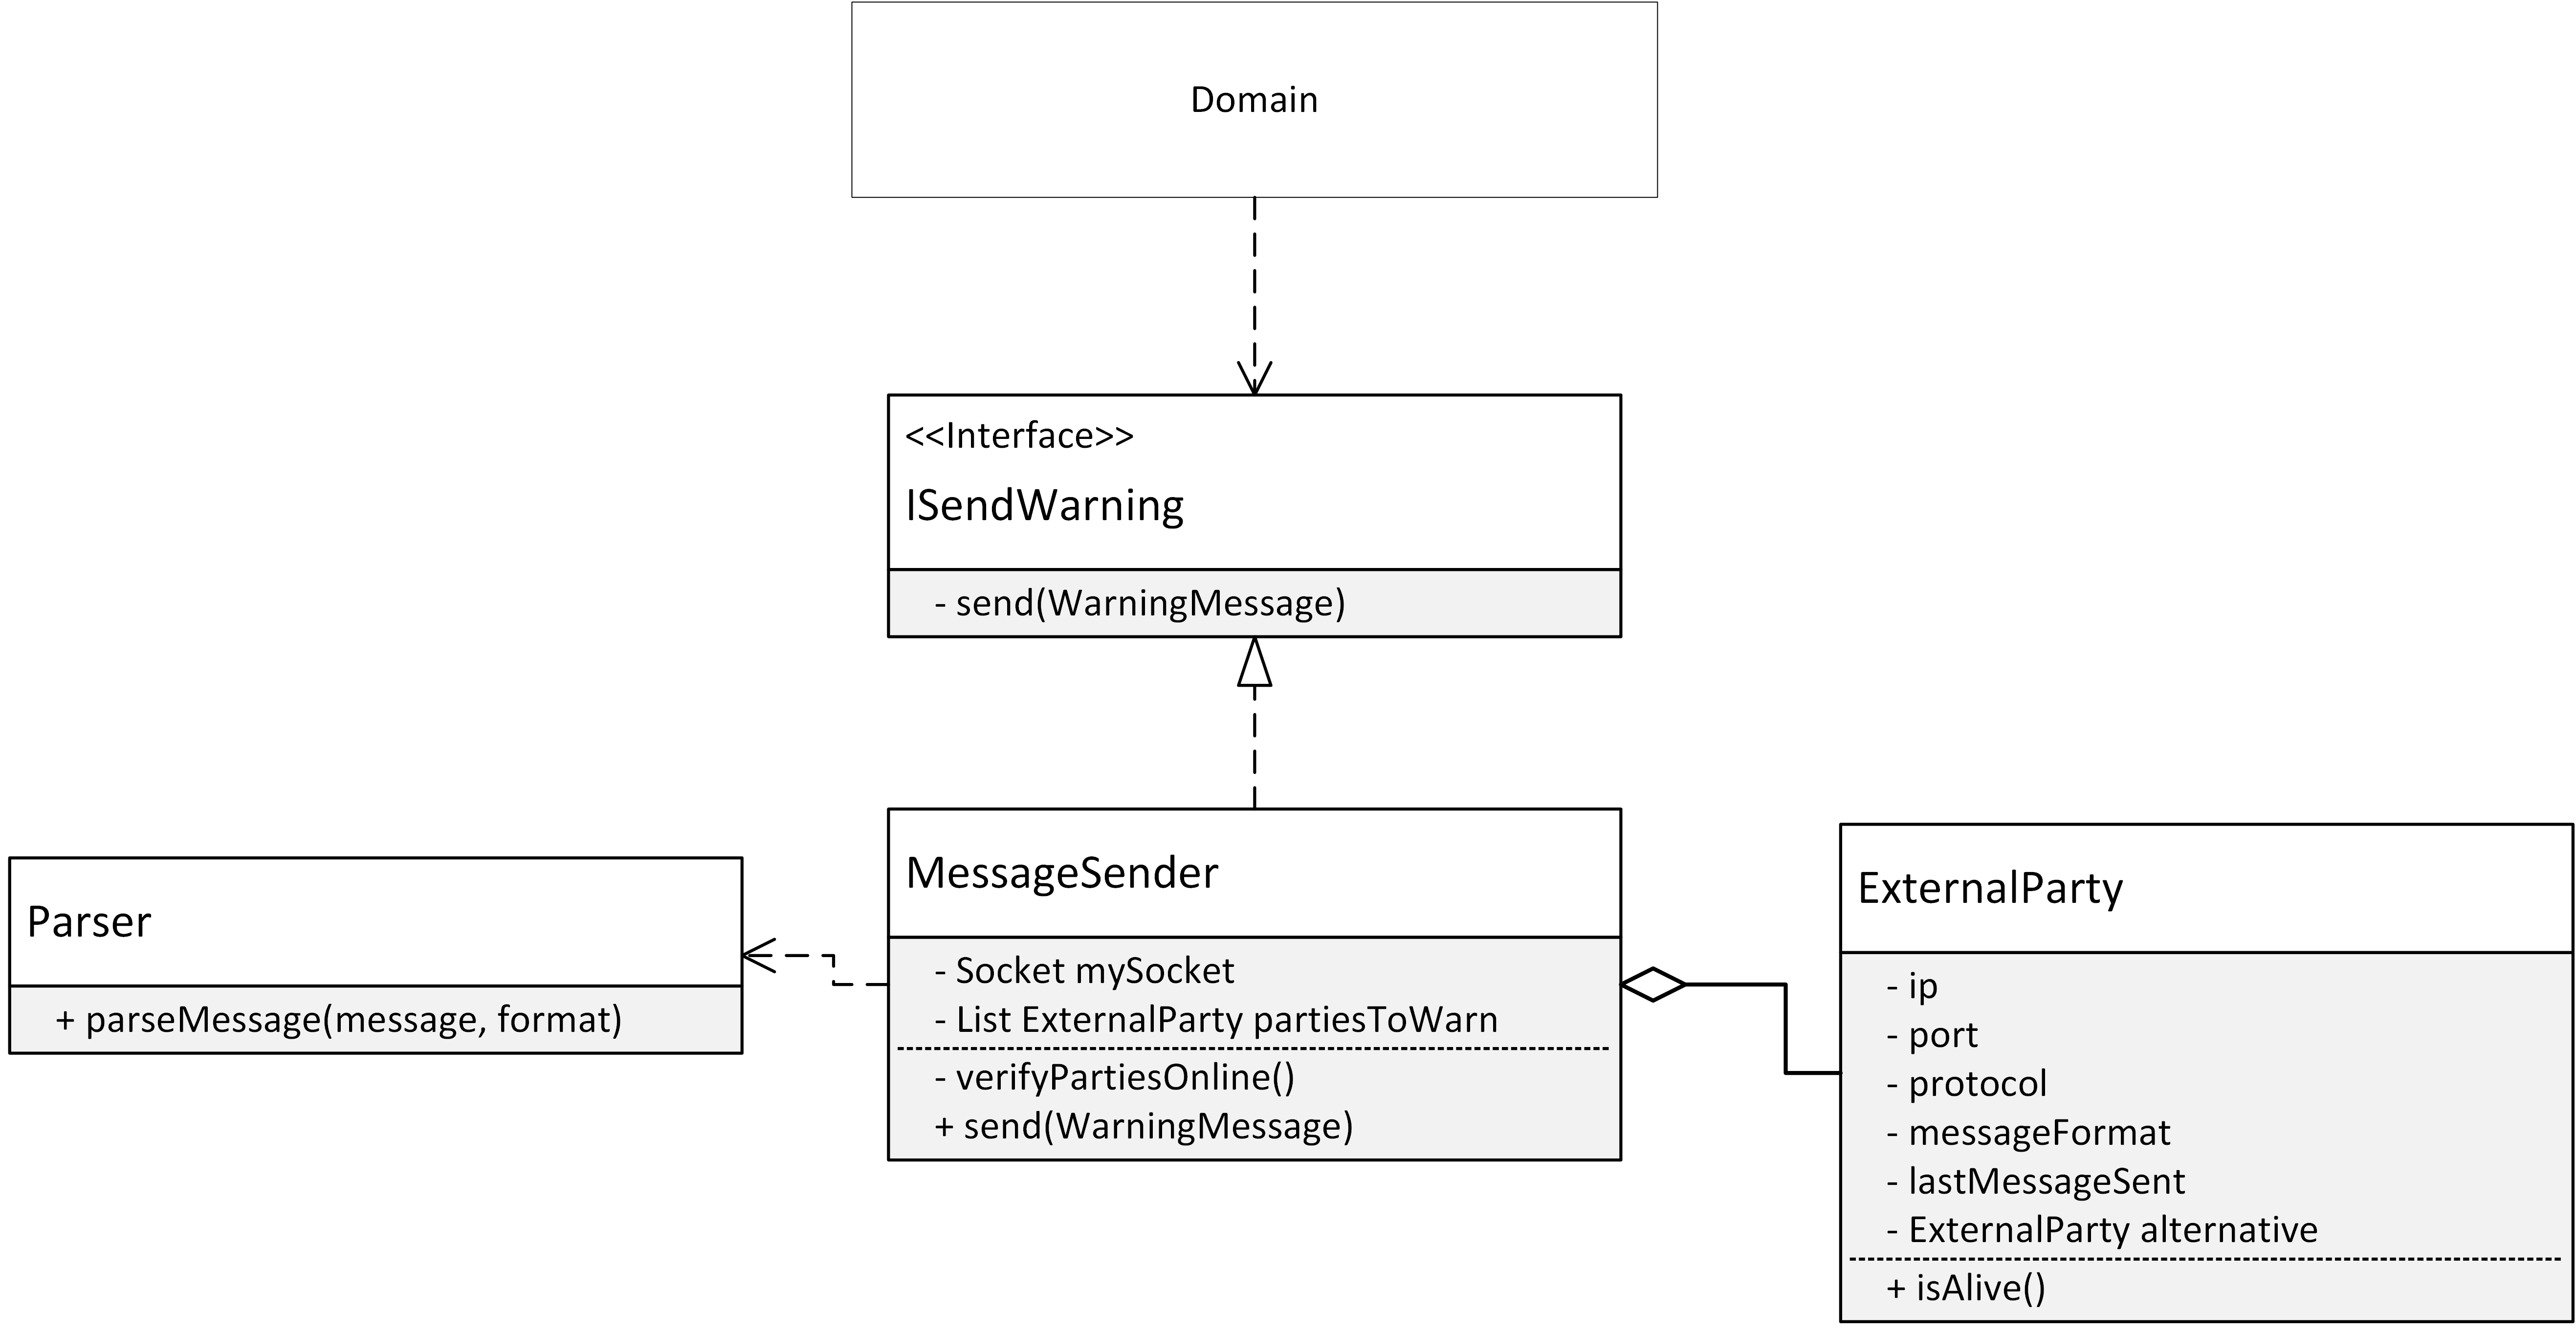
\includegraphics[keepaspectratio=true,width=1.0\textwidth]{{\viewimages/service1}.jpg}
	\caption{Class diagram of service layer}
	\label{fig:service1}
\end{figure}

In figure~\ref{fig:sequence-sensordata} a sequence diagram of sending the sensor data can be seen. As elaborated in decision~\ref{dec:5}, the sensors will push their data to the server. The sensor has two running threads: one reading the measurements and the other for sending the data every 60 seconds.

\begin{figure}[H]
	\centering
	\includegraphics[keepaspectratio=true,width=0.7\textwidth]{{\viewimages/sequence_sensor}.png}
	\caption{A sequence diagram of sending the sensor data}
	\label{fig:sequence-sensordata}
\end{figure}

\textbf{\textsc{URL}}
\begin{lstlisting}
/monitor/{monitorid}/sensorvalues
\end{lstlisting}

\textbf{\textsc{REQUEST HEADERS}}
\begin{lstlisting}
Content-Type: application/json
Authorization: <<Hash>>
\end{lstlisting}

\textbf{\textsc{REQUEST BODY}}
\begin{lstlisting}
[
	{
		sensor: "<<sensorid>>",
		value: "<<value>>"
	},
	{
		sensor: "<<sensorid2>>",
		value: "<<value2>>"
	},
	...
]
\end{lstlisting}


%TODO (should push/pull be a decision?)
%TODO (HMAC should be a decision, could also use other hashes and verification)

The arduino system only pushes the data to the server. This push model reduces the load of the arduino systems because there are no incoming requests. This way, the arduino also doesn't have to store or manage any data, which also means the arduino doesn't need security measurements to secure this data.\\
The server does however need to verify that the messages it receives from the arduino monitoring systems are in fact send by our arduino systems. Otherwise a hacker could send sensor messages too, which would jeopardize the entire flood warning system.The downside to having the arduino systems push the data, is that data will be received by the server was not needed or wanted. Defect sensors data will still be send. \\
%http://rc3.org/2011/12/02/using-hmac-to-authenticate-web-service-requests/
% HMAC suggested by microsoft: https://msdn.microsoft.com/en-us/library/dd203052.aspx
 
The message security is done by using a hash based message authentication code (HMAC) using SHA-256 as the hashing algorithm. Upon receiving the messages, the service layer verifies the message before further processing the message.\\
The sequence of actions for obtaining information from SFM is shown below in figure \ref{fig:getinfosfm}.
\begin{figure}[H]
	%\centering
	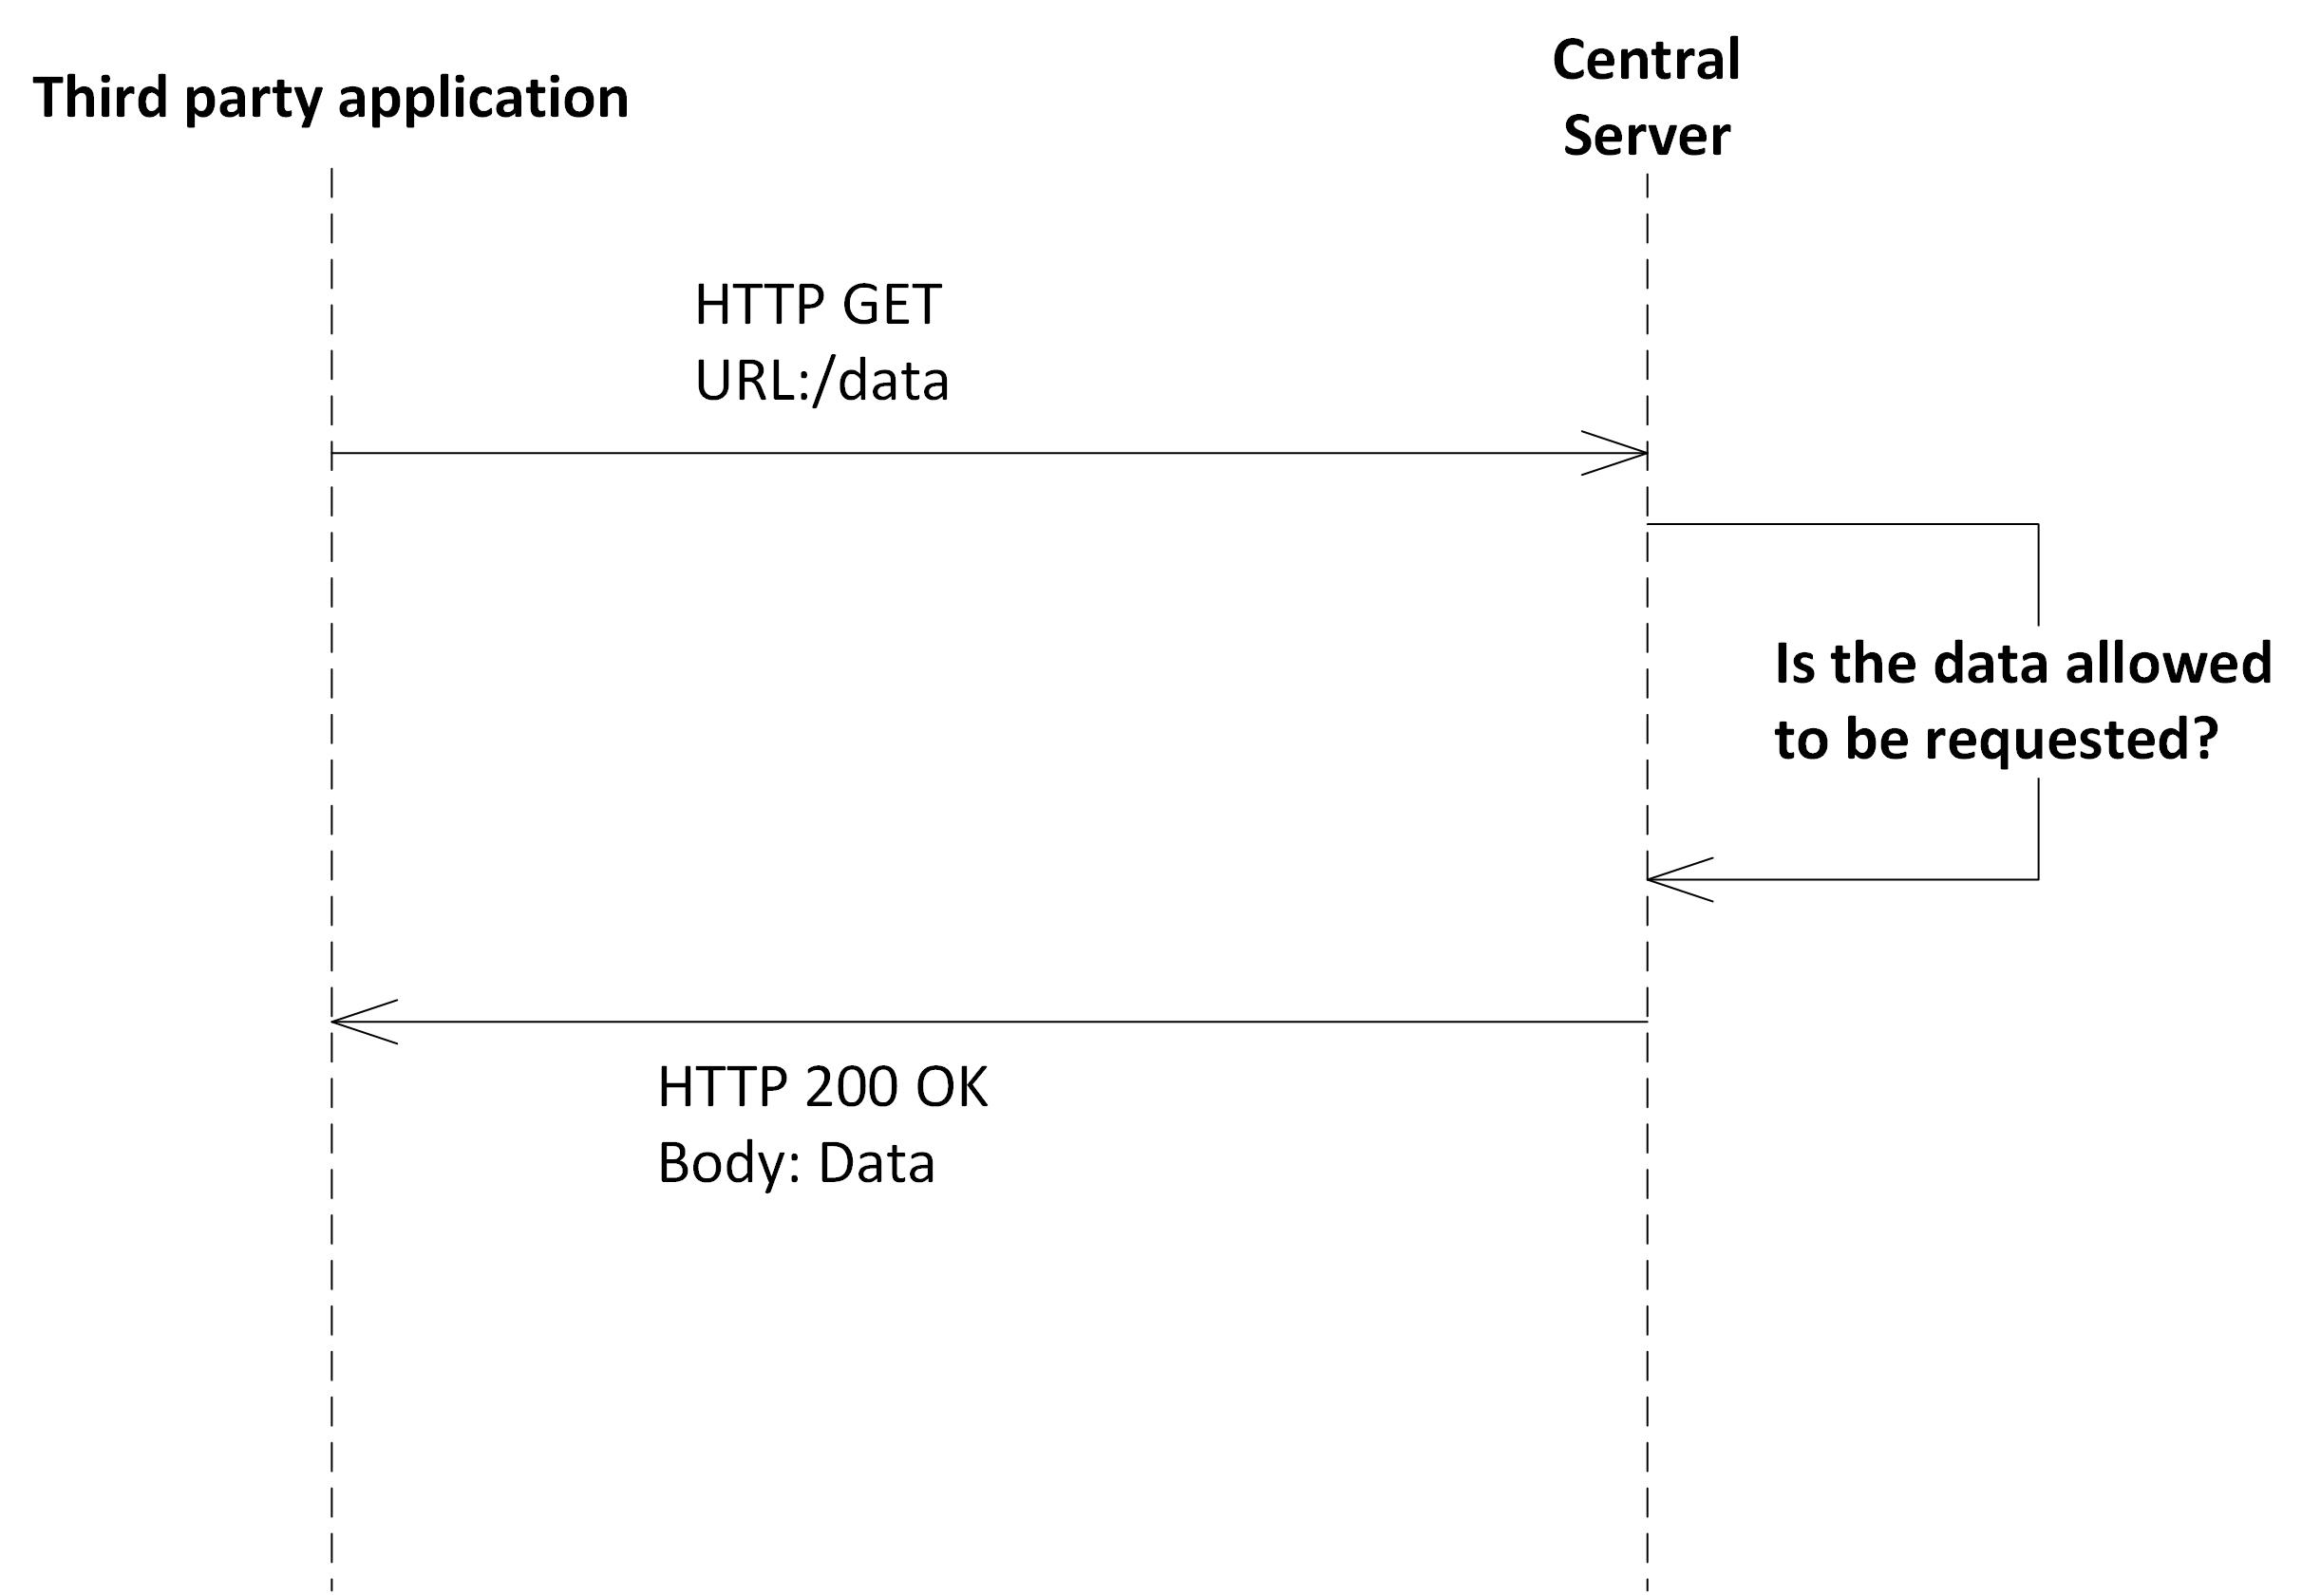
\includegraphics[keepaspectratio=true,width=0.9\textwidth]{{\viewimages/sequencethirdparty}.jpg}
	\caption{Sequence diagram of 3rd party obtaining data from SFM}
	\label{fig:getinfosfm}
\end{figure}

The API calls the service layer receives that request information, don't need to be authenticated. These calls, however, do need to be limited by the service layer to not be able to delete or modify information. The information the API provides is defined in the server layer and the API does not return any information other then that.\\
The third party sends a HTTP GET request to the REST server of SMF. Upon receiving this request, the REST server checks if the request is secure. This logic is located in the service layer. When the request is secure, the REST server calls the mapper object in order to get the requested data. The mapper object first checks the identity map if the data is already loaded. This will reduce the amount of queries executed on the database. If this identity map doesn't hold the data, the mapper sends a query to the database. The data returned from the database is then returned to the REST server, who sends the data to the third party.

\paragraph{Distribute warnings}
In figure~\ref{fig:warning} a sequence diagram of sending warnings to the emergency room and citizens can be seen. The sequence diagram contains a time constraint of 10 seconds and 5 minutes, for warning the emergency room and all citizens respectively.

\begin{figure}[H]
	\centering
	\includegraphics[keepaspectratio=true,width=1.0\textwidth]{{\viewimages/sequence_warning}.png}
	\caption{A sequence diagram of sending warnings to citizens and emergency room}
	\label{fig:warning}
\end{figure}

%							Downside: Data will be received that was not requested, even if not interested. 
%Three principal layers (p20 poeaa)

\subsubsection*{Domain layer}
The domain layer contains all the logic of the system. This includes the logic for the algorithms used to decide if a warning should be issued. And it includes the logic for managing the sensor data.\\
The sensor manager checks if the sensor is still working correctly.%todo
If the sensor is working correctly, the sensor data gets stored and processed.\\
The class diagram for handling incoming REST server calls is shown in figure \ref{fig:domain1}.
\begin{figure}[H]
	\centering
	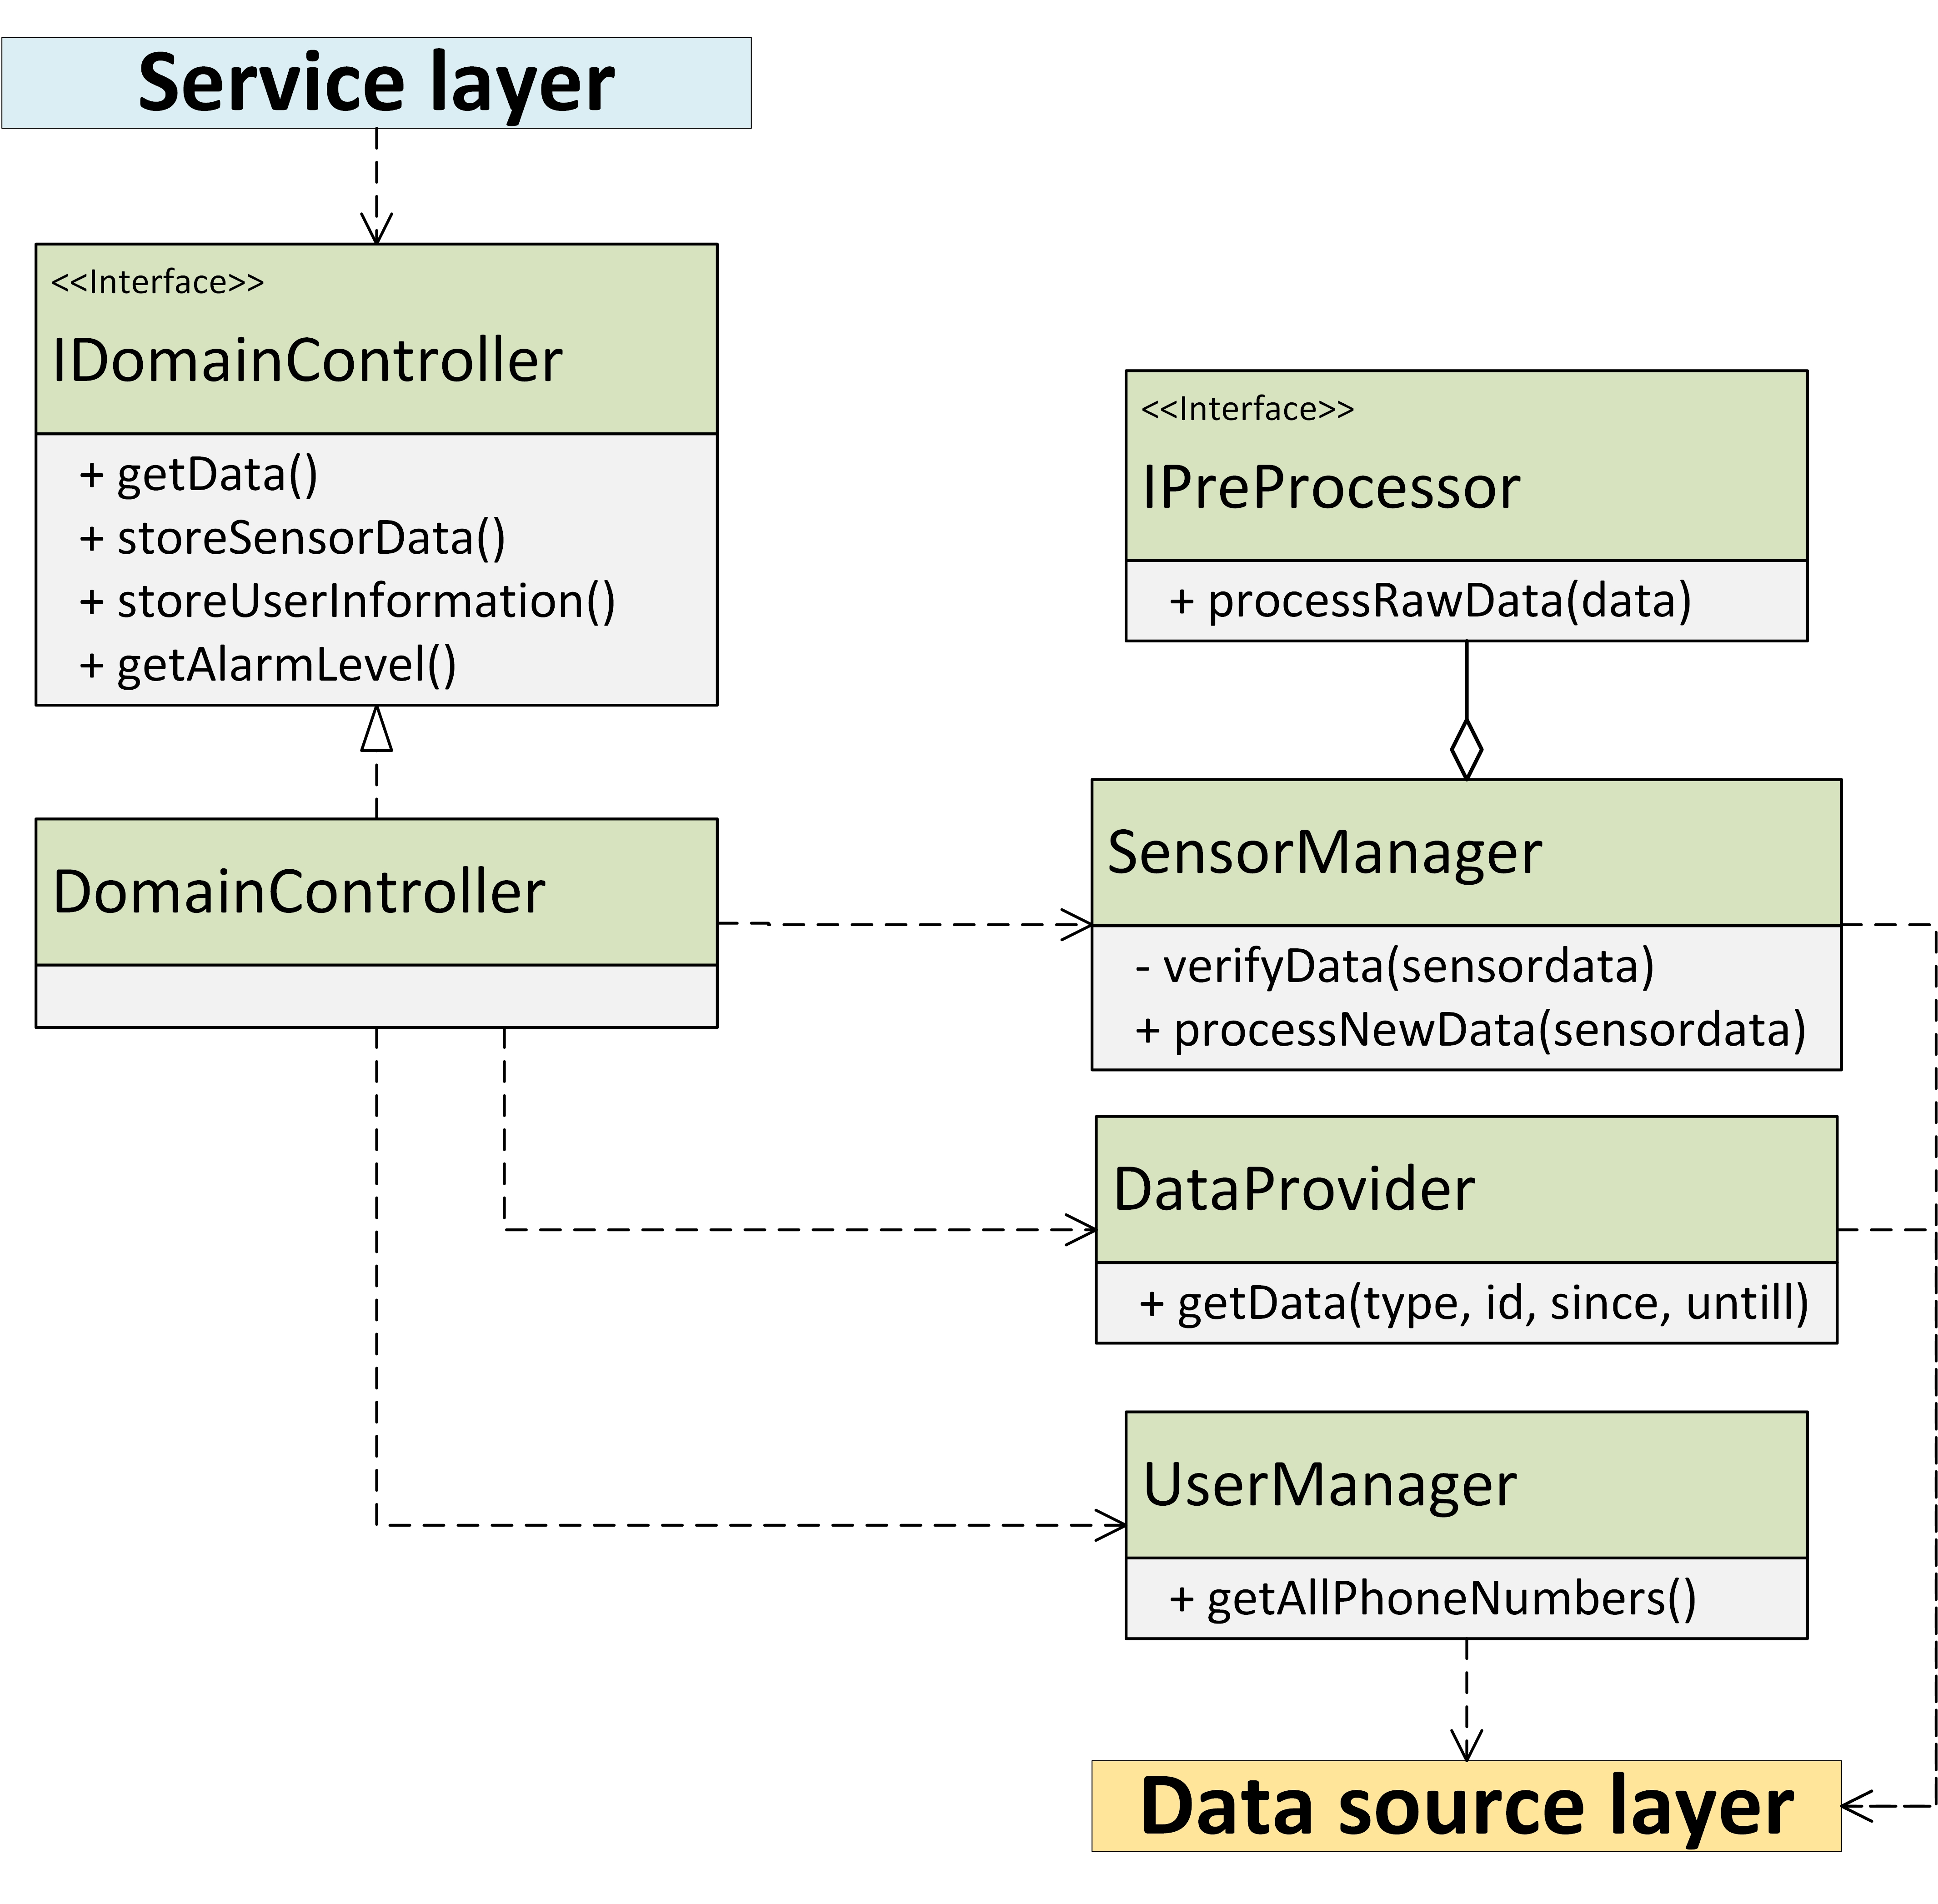
\includegraphics[keepaspectratio=true,width=1.0\textwidth]{{\viewimages/domain1}.jpg}
	\caption{Class diagram of the domain layer concerning REST calls}
	\label{fig:domain1}
\end{figure}

The class diagram of the algorithm processing the data is shown below in figure \ref{fig:domain2}

\begin{figure}[H]
	\centering
	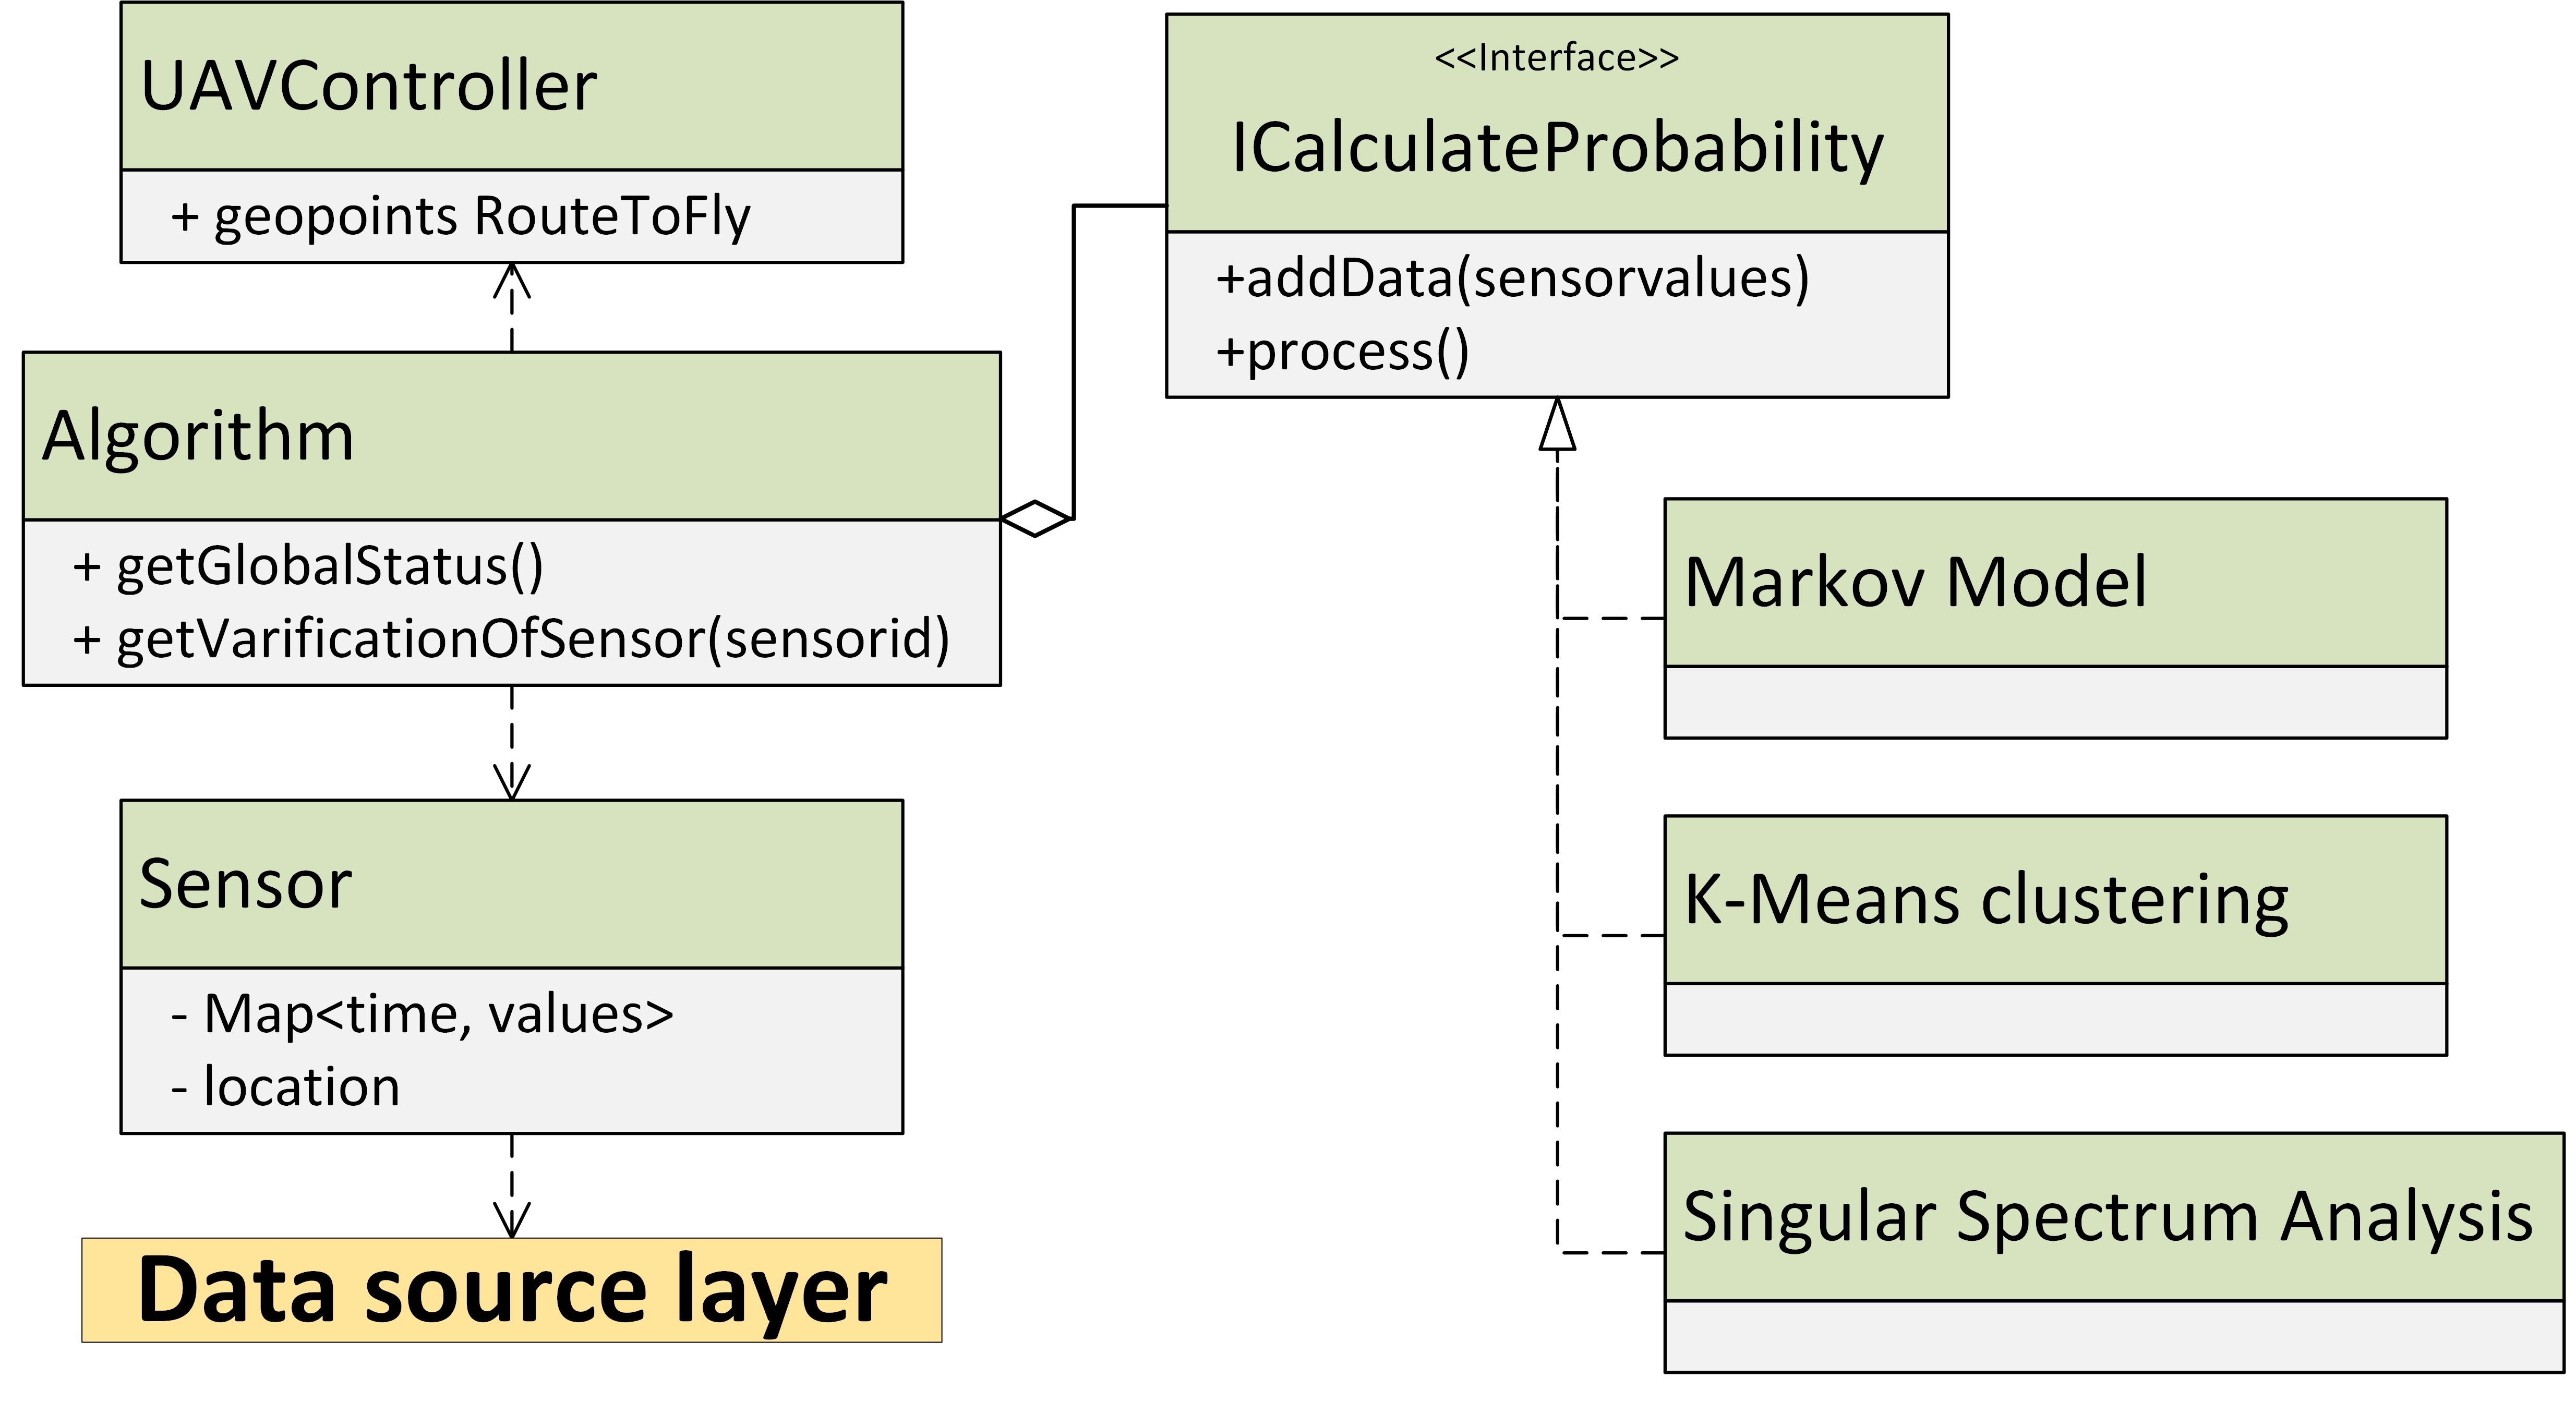
\includegraphics[keepaspectratio=true,width=1.0\textwidth]{{\viewimages/domain2}.jpg}
	\caption{Class diagram of flood prediction in the domain layer}
	\label{fig:domain2}
\end{figure}
First the incoming sensor data is getting pre processed. 
This is done by using:
\begin{itemize}
	\item Smoothing the L1 norm using the Huber function 
	\item Hodrick–Prescott filter
\end{itemize}

The the L1 norm smoothing fluctuates more than the Hodrick-Prescott function. This way, the long term and short term differences can be analyzed better.\\

%https://en.wikipedia.org/wiki/Hodrick%E2%80%93Prescott_filter
%http://mathoverflow.net/questions/118333/smoothing-l1-norm-huber-vs-conjugate
%
After the pre processing, the sensor data gets stored and will be used in several algorithms to calculate a flood probability.
There are several algorithms being used, these are:
\begin{itemize}
	\item Hidden Markov model with k-means clustering
	\item Singular Spectrum Analysis (SSA) for locations with tides
	\item Limit checking
\end{itemize}

Limit checking is just checking if the value of the sensor is not above a certain limit. A sudden extreme value will be detected using limit checking. If there are more sensors giving extreme values, the domain layer will verify this sudden change and might then issue the service layer to send a warning message.\\
SSA splits the range of values into blocks and then checks for abnormalities within that block.\\
The k-means clustering algorithm is used to detect abnormalities in the sensor data coming from a certain range dike. This way all the sensors should measure about the same values. In order to check for abnormalities, the k-means clustering can detect when a sensor value is out of the cluster.\\

%corrdata slide 60
How strongly correlated two types of data are will be calculated using Longitudinal Data Analysis.

\subsubsection*{Data source layer}
The data mapper \cite{Fowler:2002:PEA:579257} is used to completely separate and ignore the database in the domain model. The domain object only uses an interface to a "find" function that returns the requested object. This could be either from the database or from the internal memory.\\
How the database is structured will be discussed in the implementation view section.

% \begin{figure}[H]
% %\centering
% 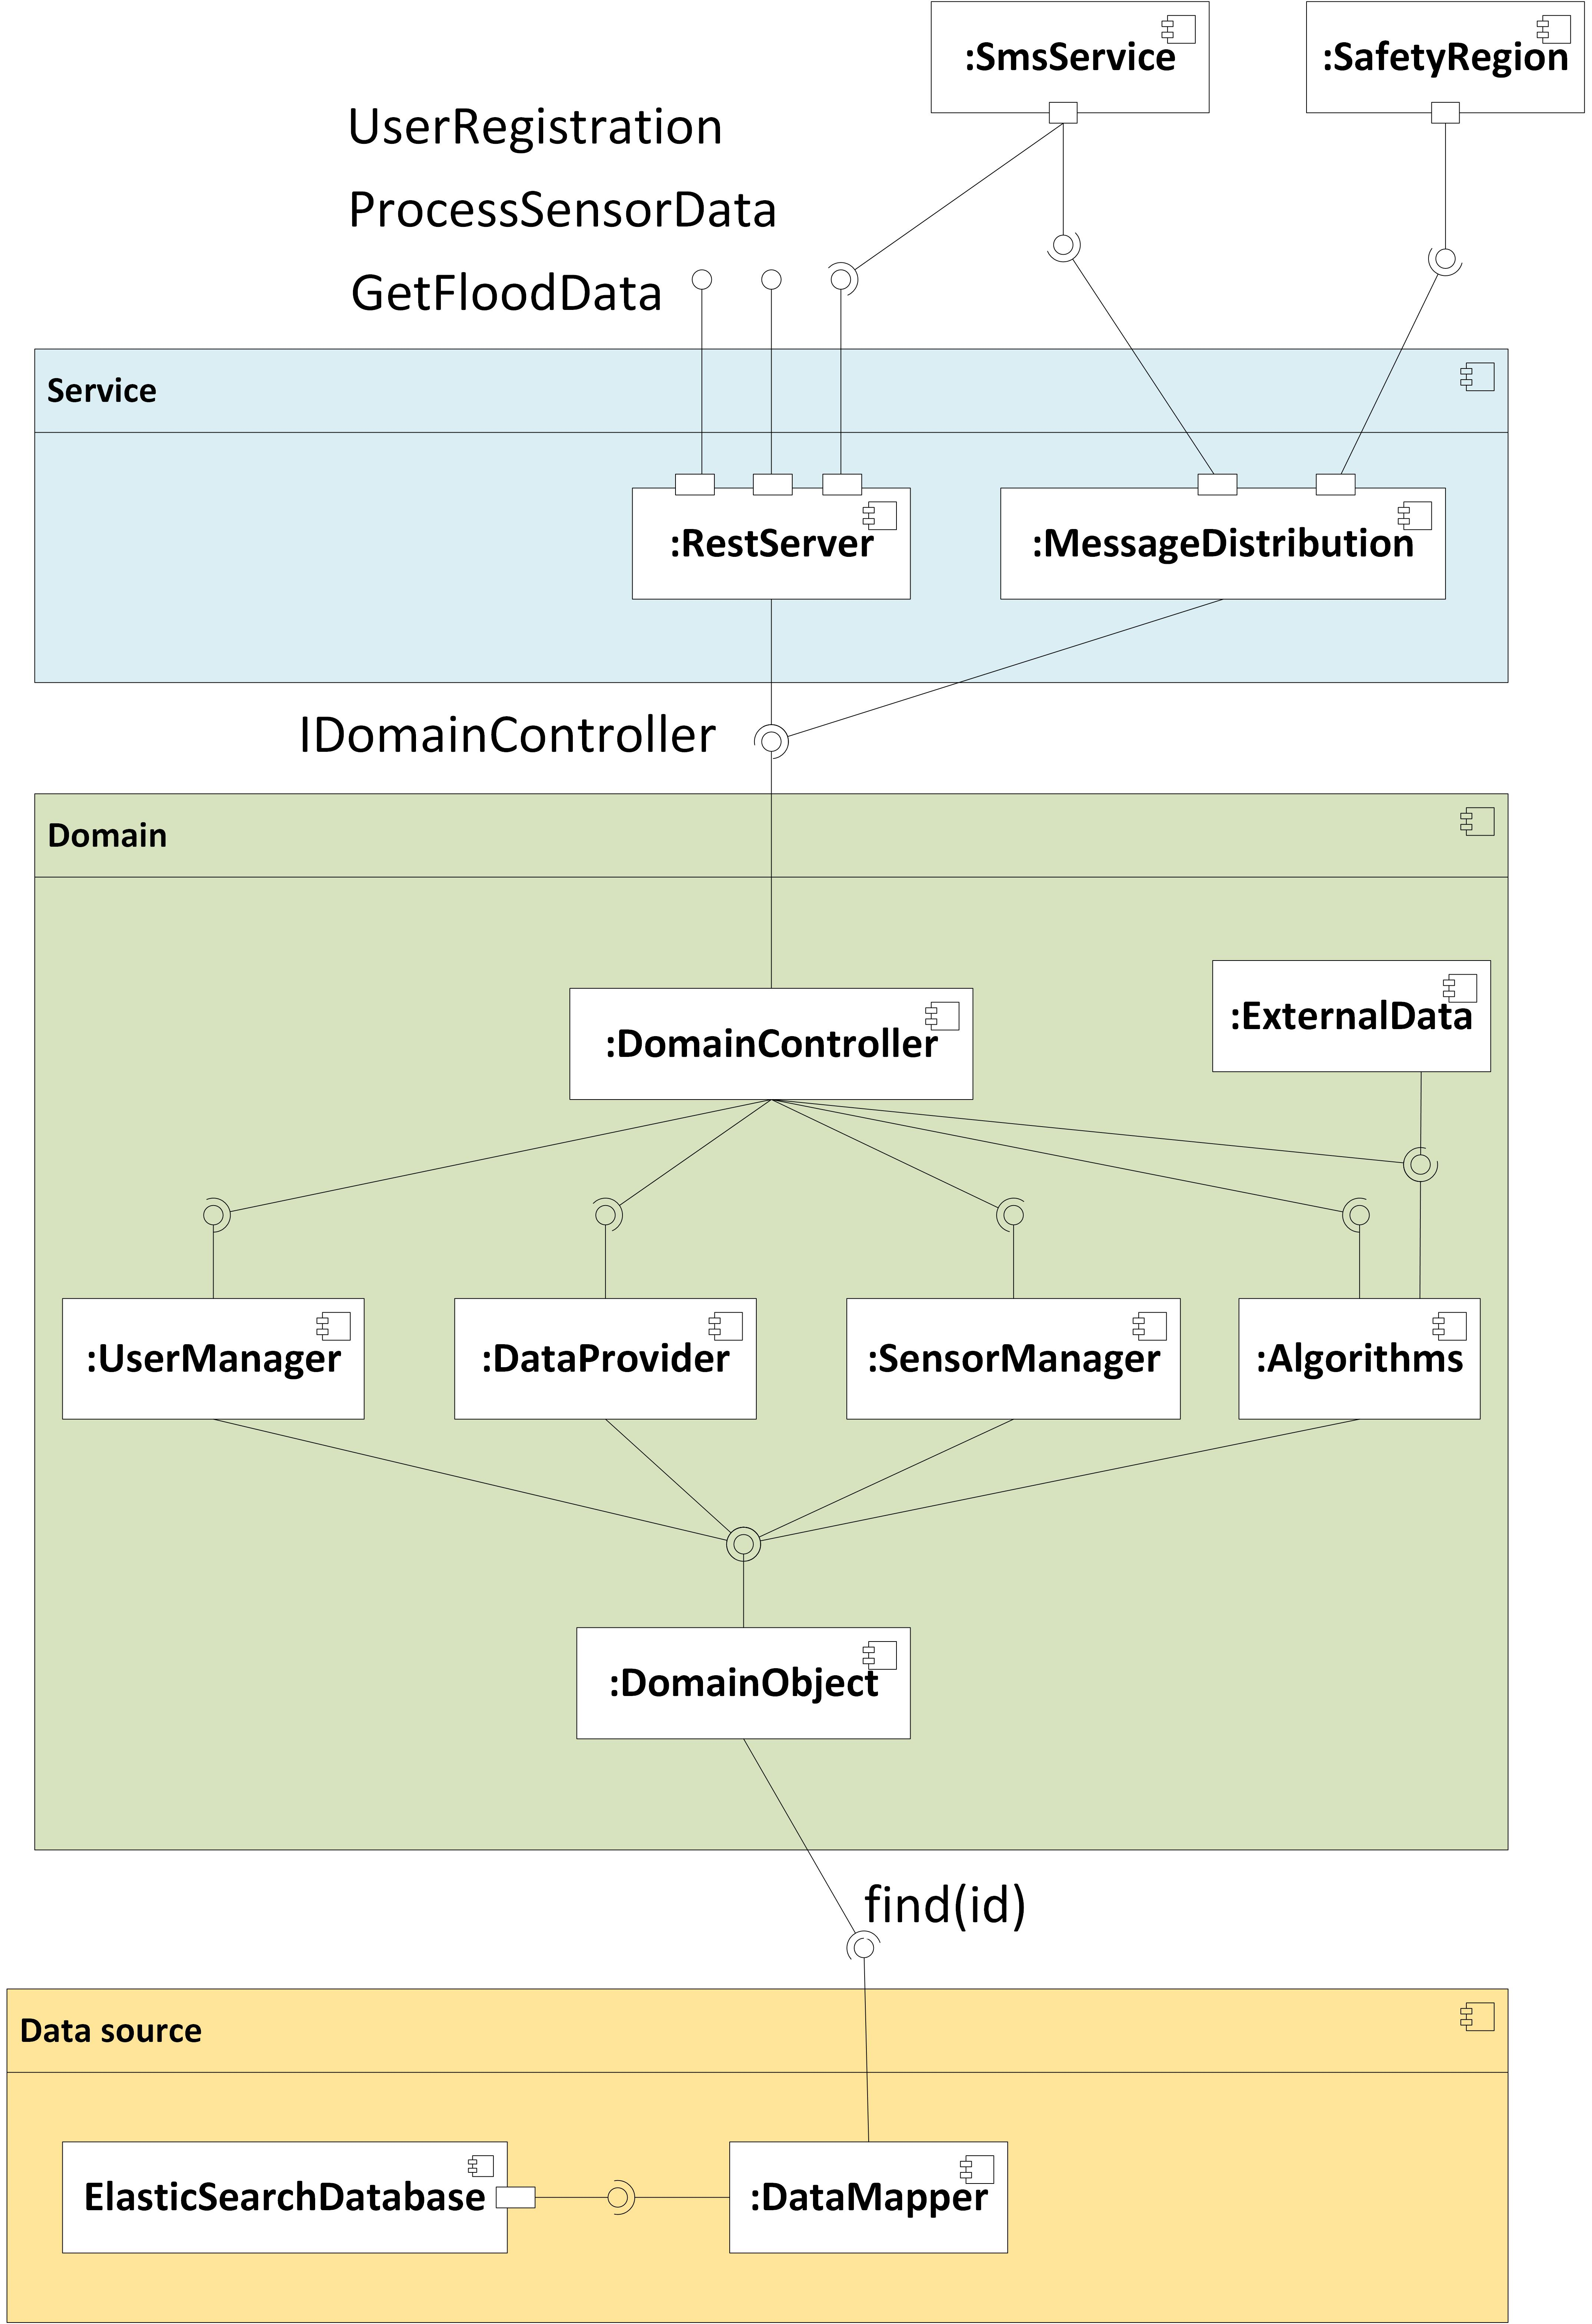
\includegraphics[keepaspectratio=true,width=0.9\textwidth]{{\viewimages/component}.jpg}
% \caption{Component diagram}
% \label{fig:component}
% \end{figure}



% \clearpage
% \begin{figure}[H]
% %\centering
% 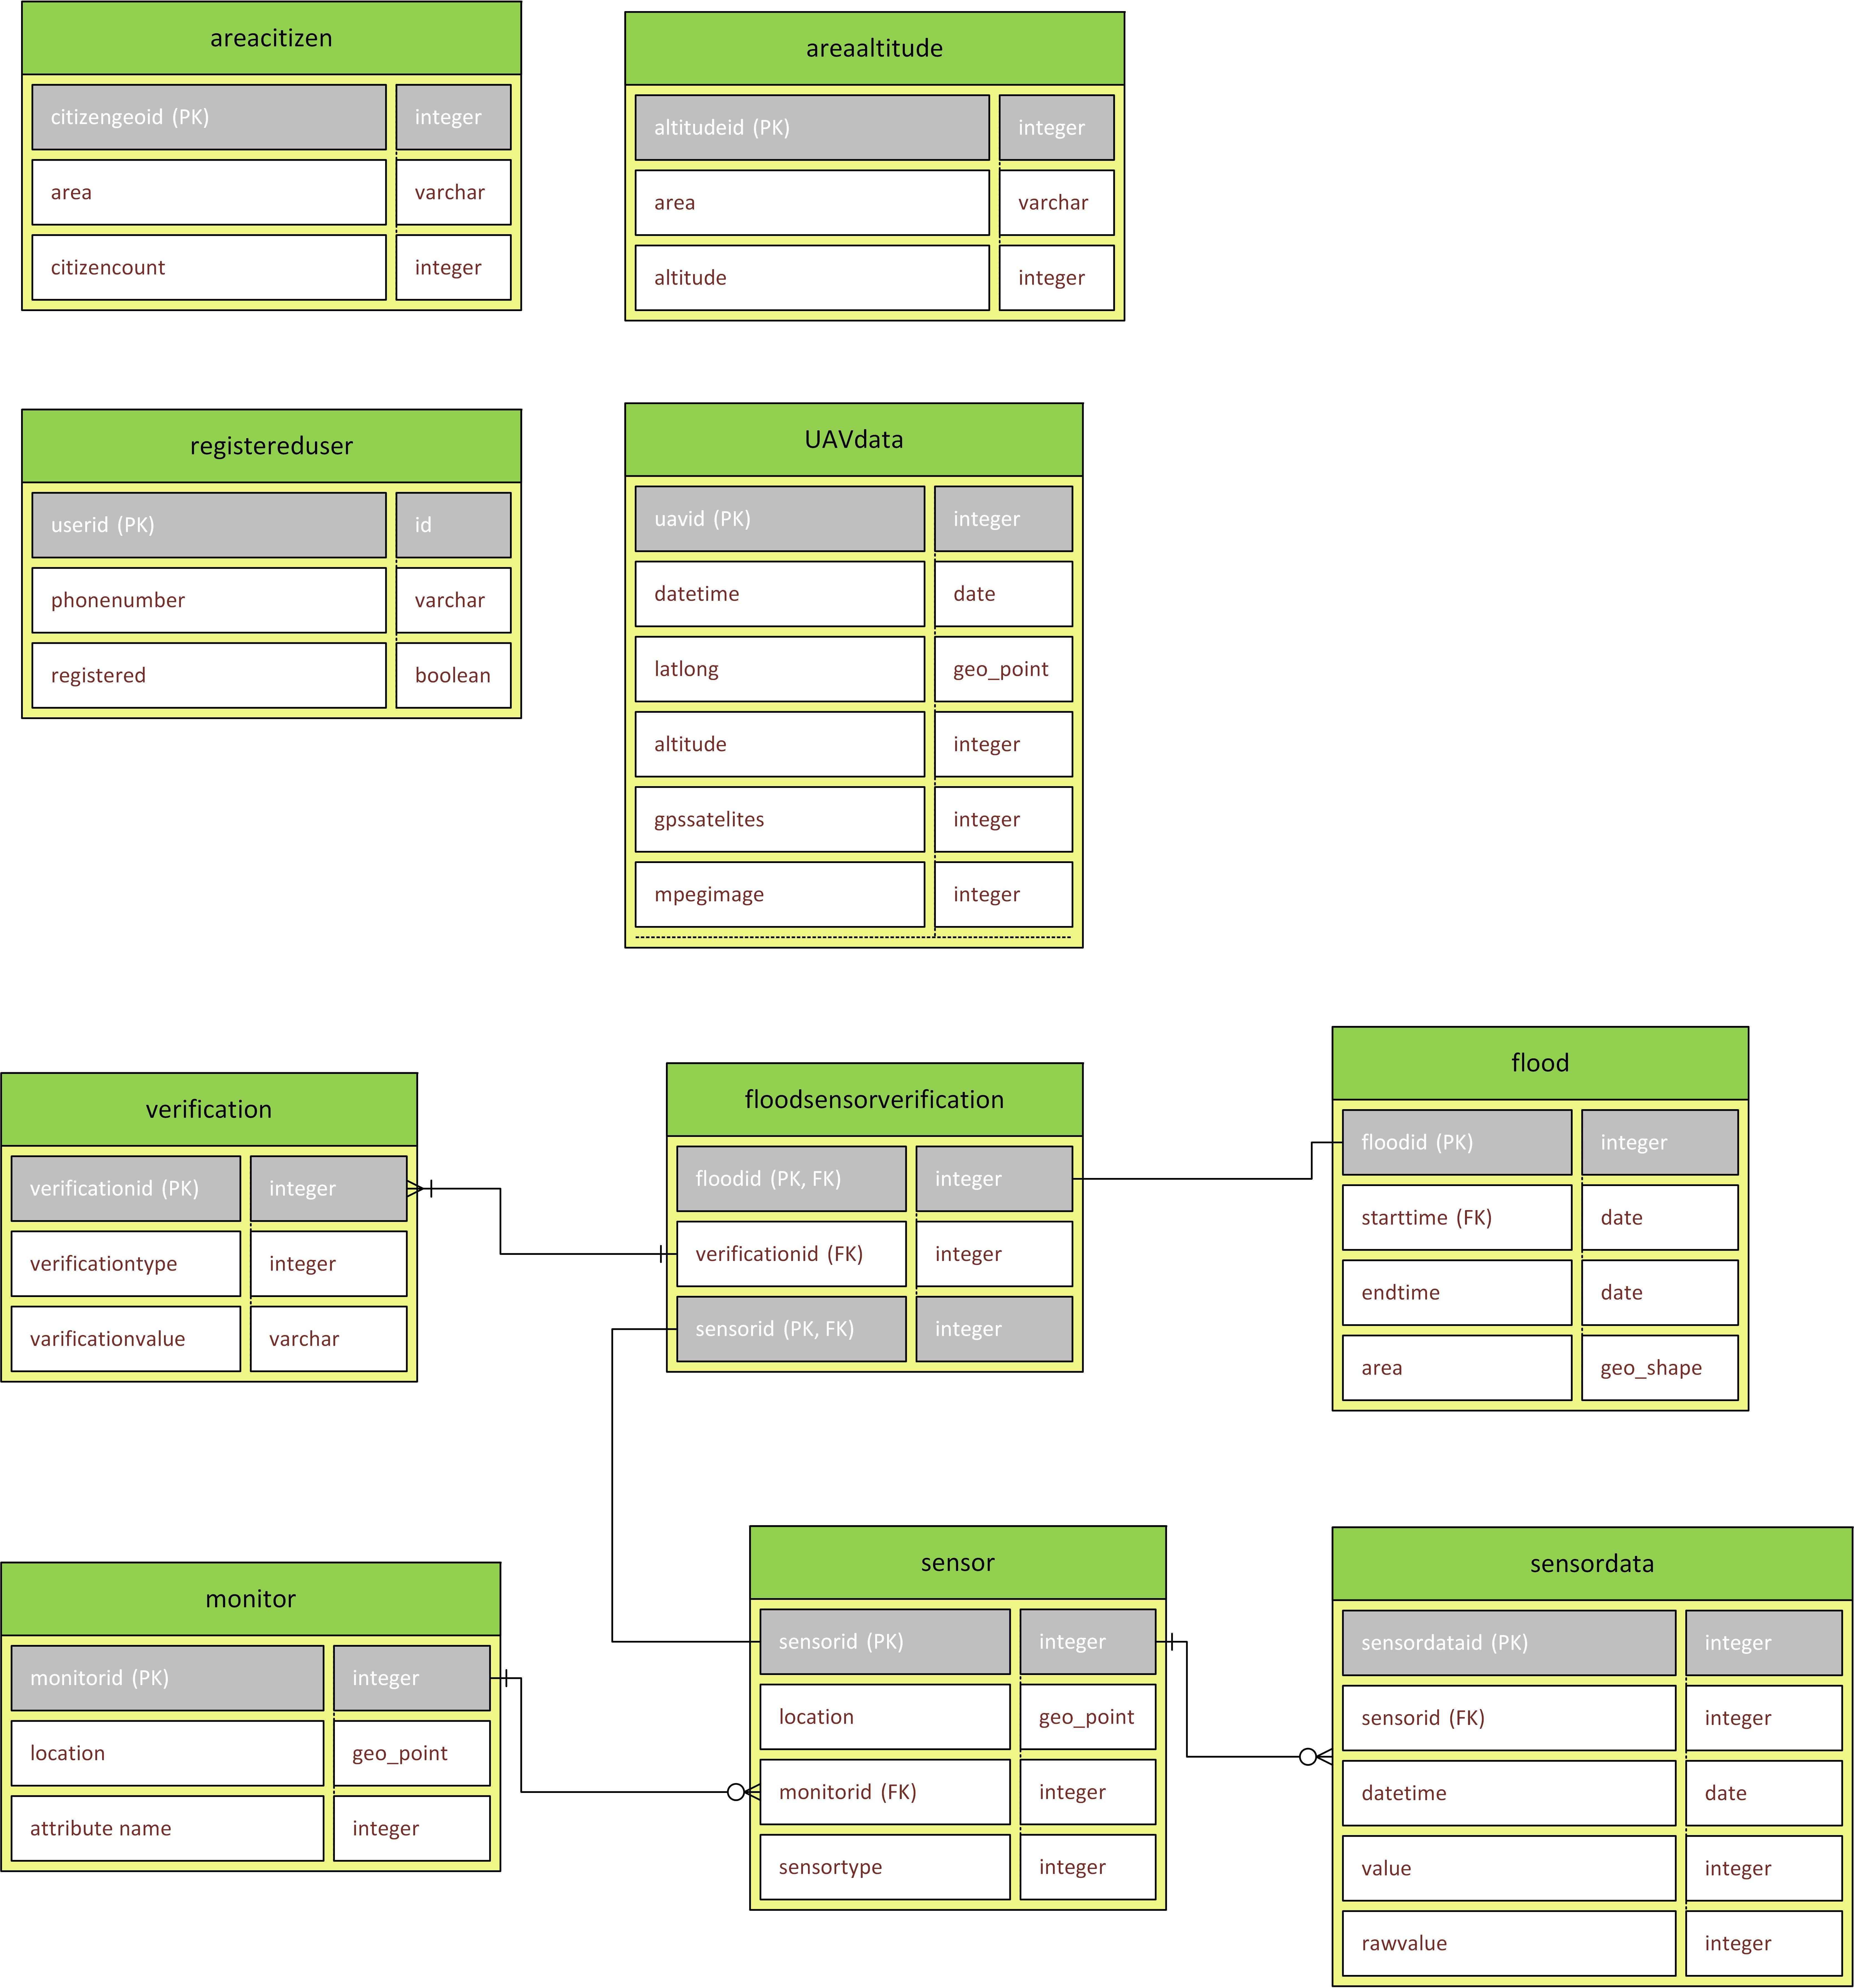
\includegraphics[keepaspectratio=true,width=0.9\textwidth]{{\viewimages/database}.jpg}
% \caption{Database diagram}
% \label{fig:component}
% \end{figure}

% \begin{figure}[H]
% %\centering
% 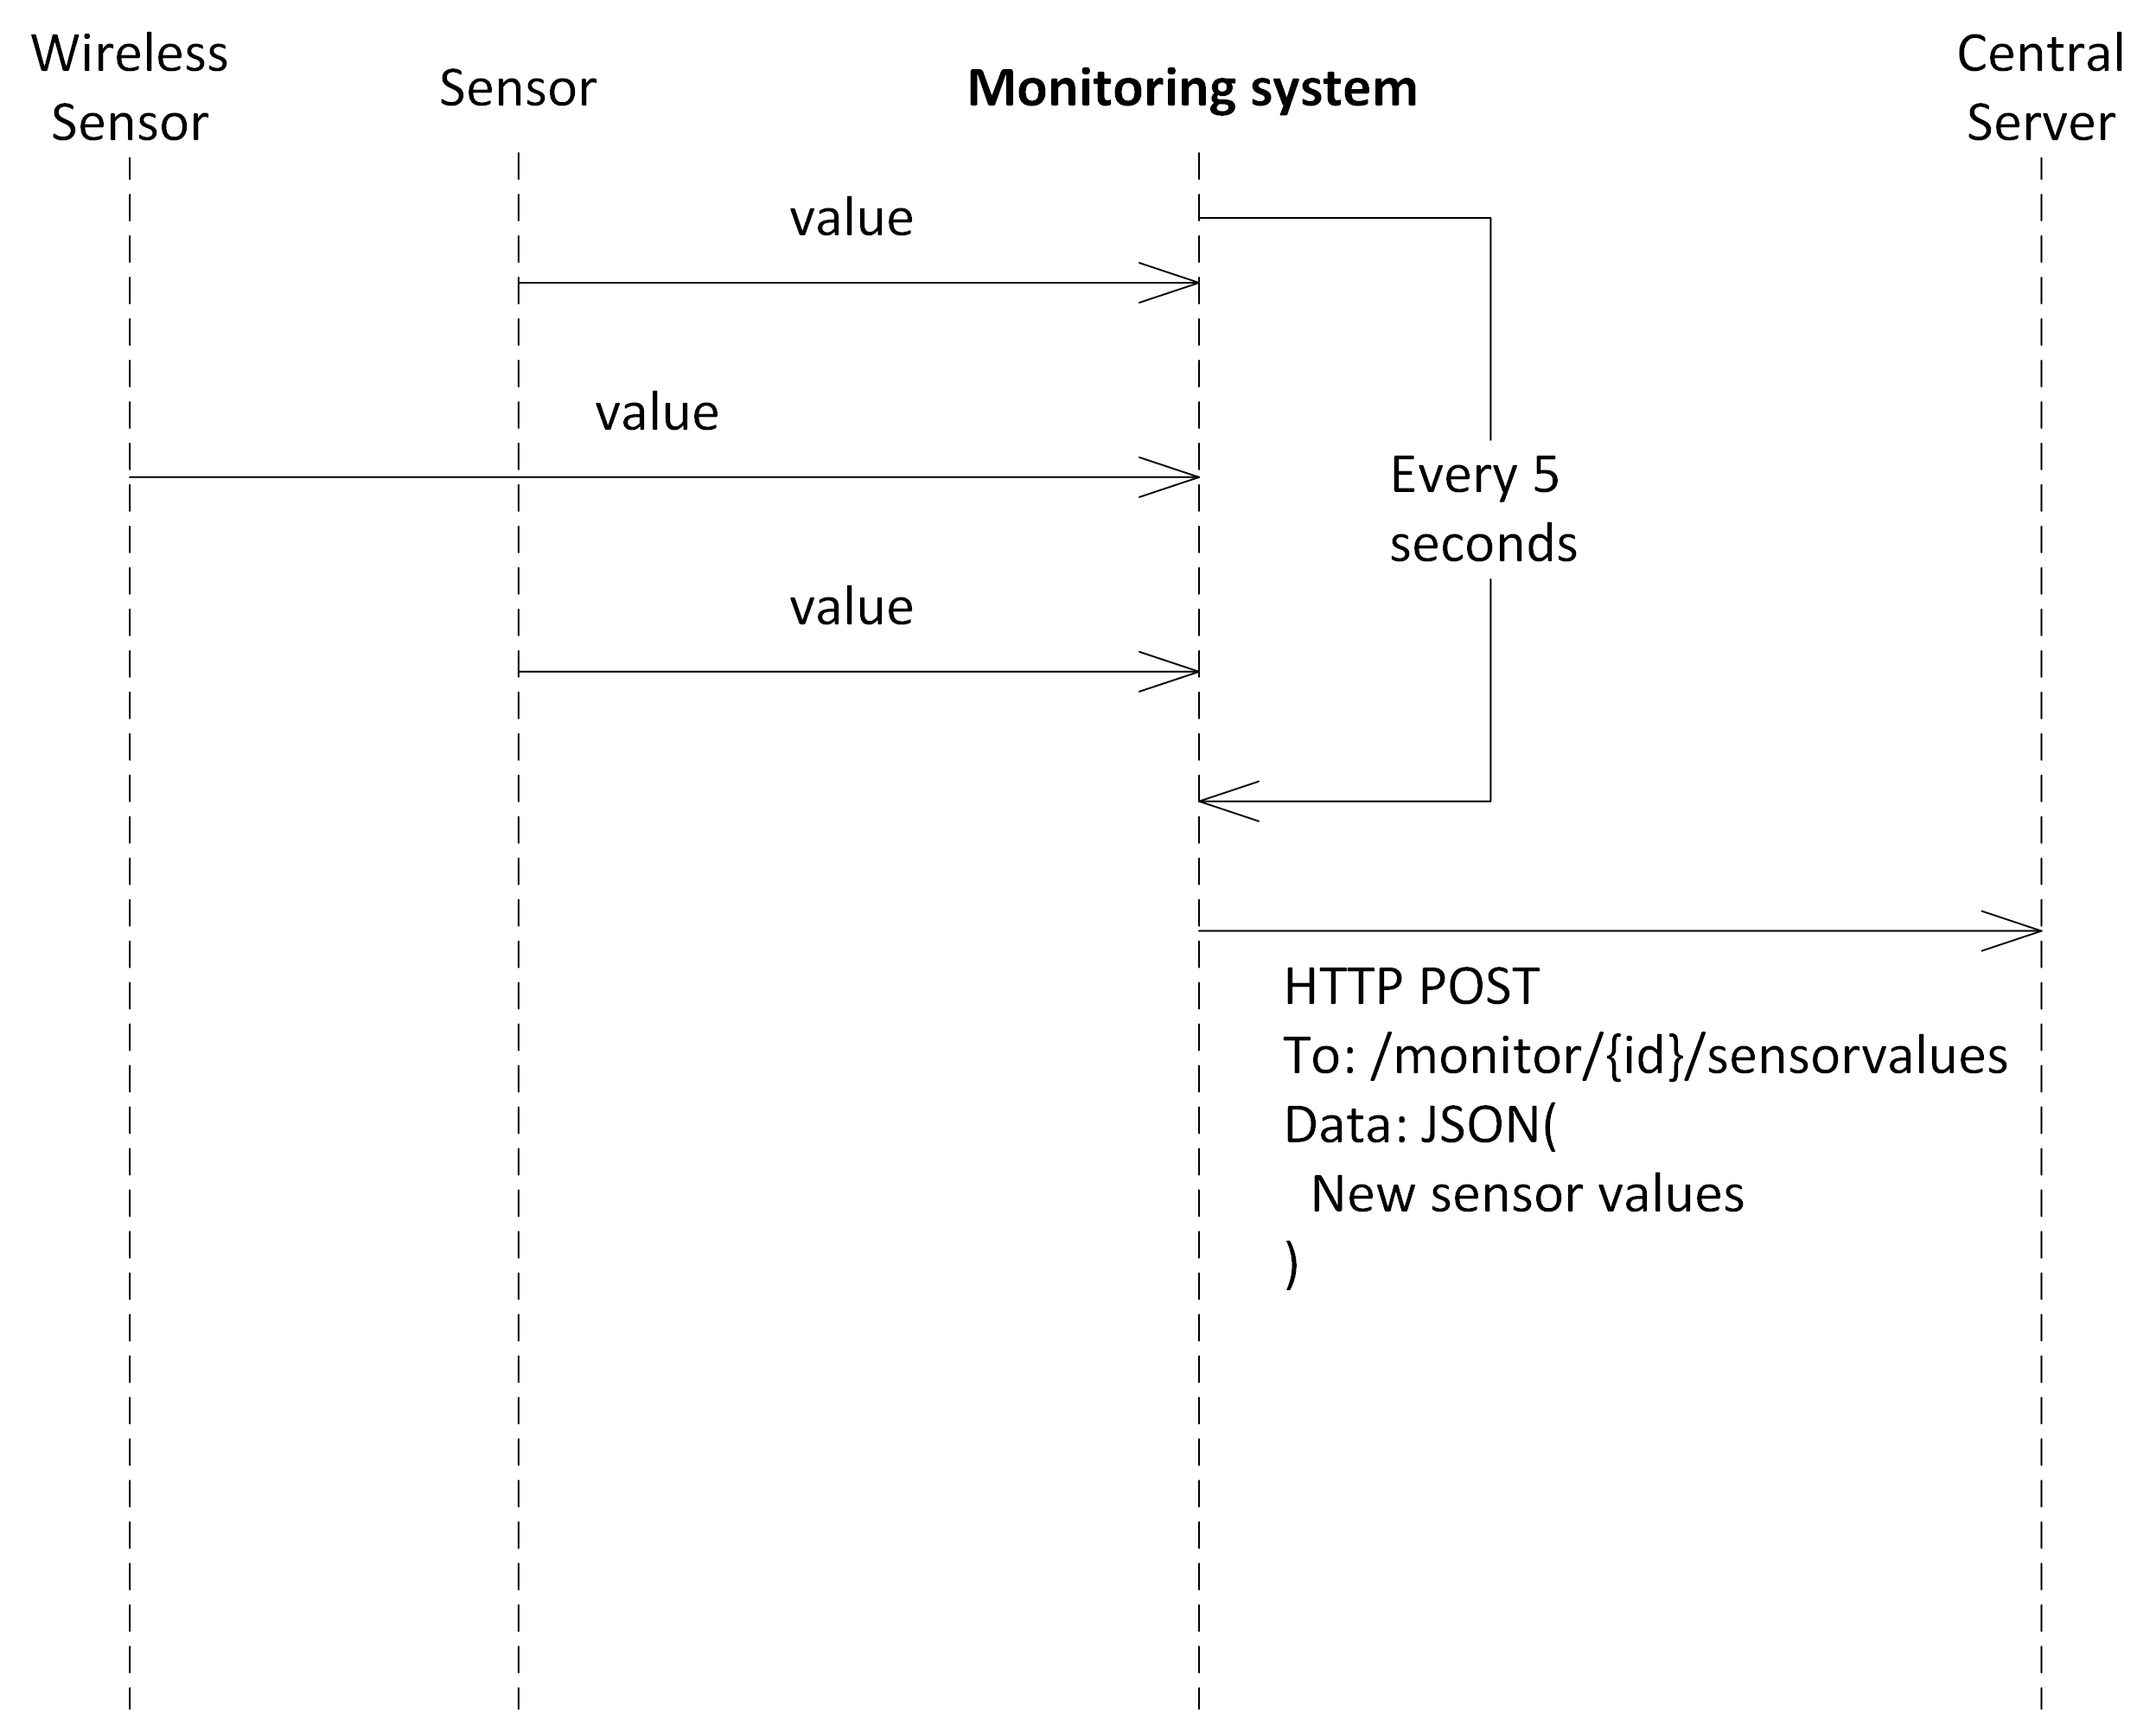
\includegraphics[keepaspectratio=true,width=0.9\textwidth]{{\viewimages/sequence1}.jpg}
% \caption{Sequence diagram of the client pushing the sensor data}
% \label{fig:component}
% \end{figure}
%\begin{framed}
%
%	Update monitor system firmware? Do we do this? And how do we do this?
%	Do sensors have firmware and how do we update that?
%
%\end{framed}



\clearpage
\subsection{Implementation view}
\copied{The development view illustrates a system from a programmer's perspective and is concerned with software management. This view is also known as the implementation view. It uses the UML Component diagram to describe system components. UML Diagrams used to represent the development view include the Package diagram.}
{from wikipedia\\\url{https://en.wikipedia.org/wiki/4\%2B1_architectural_view_model}}

The implementation view, also known as the development view, describes the system from the programmer's perspective. This includes a description of the components of the system and how the system is packaged.  

\subsubsection{Components}
The system consists of a set of components tat all interact with each other. In figure~\ref{fig:component} below, these different components are shown. Each component can provide interfaces and uses sockets to connect to interfaces of other components. This way, the implementation of each component can independently be replaced and deployed. 

\clearpage
\begin{figure}[H]
	%\centering
	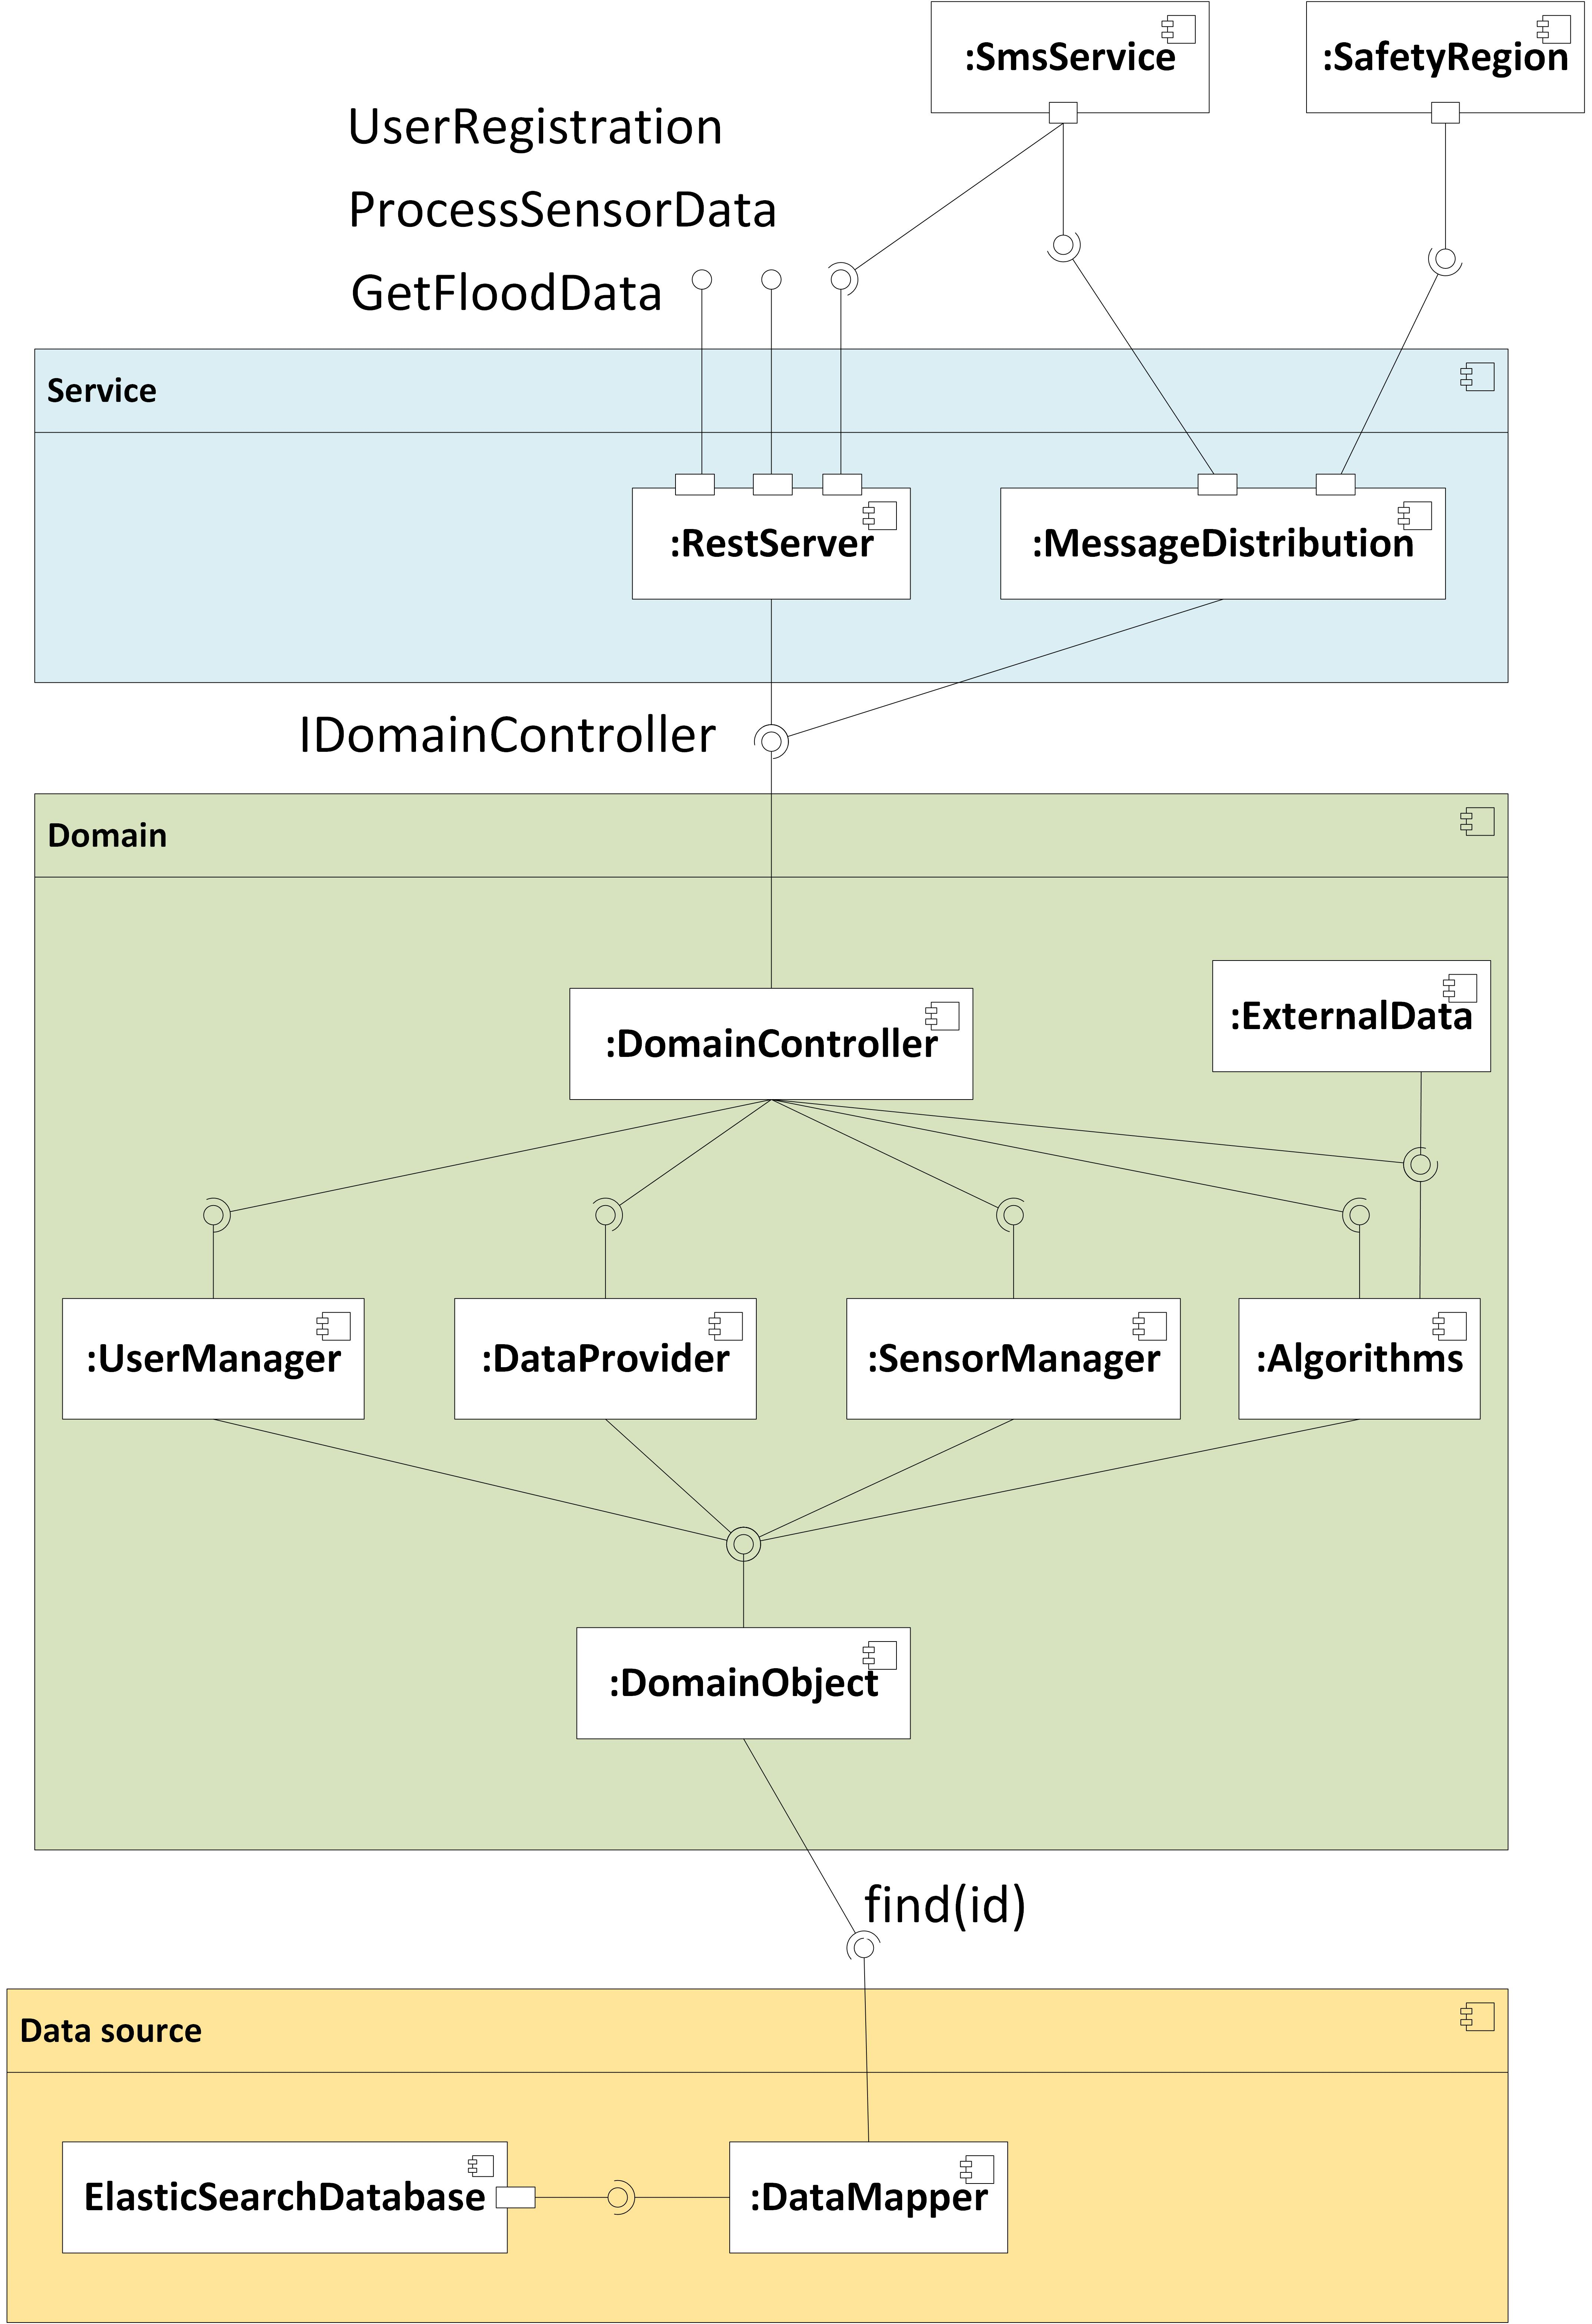
\includegraphics[keepaspectratio=true,height=13cm,width=0.9\textwidth]{{\viewimages/component}.jpg}
	\caption{Component diagram}
	\label{fig:component}
\end{figure}

There components are placed in three layers. The data source  layer, domain layer and service source layer.

In the data source layer the data is stored and the data mapper. It consist of two components. 
	Database: This is the database that holds all the stored data of the system.
	DataMapper: This component is responsible for reading from the database and adding new data.

In the domain layer the business rules and logic is placed. The following components are placed:
	UserData: Responsible for gathering the user data and normalizing
	SensorData: Responsible for gathering sensor data and normalizing
	FloodData: Responsible for gathering flood data and normalizing
	UAVData: Responsible for gathering UAV data and normalizing
	UserManager: Responsible for maintaining the phone numbers and other information of the registered users.
	DataProvider: Responsible for obtaining the data the REST server requests. 
	SensorManager: Component that is used for installing, update and delete sensors and retrieving data from the sensors.
	Algorithms: Component used for algorithms that calculated the flood probability.
	RESTController: Component to enable RESTful support.
	
In the Service layer the services are included used by external actors. The following components are included:
	RESTServer: Server which communicates with external software
	MessageDistribution: Component responsible for distributing warning messages to external parties.
	
Outside the layer are external software components:
	SMSService: Component to let citizen subscribe for warning texts and receive warning texts.
	SafetyRegion: Component to which the system communicates to in order to warn the Safety region.

\subsection{Database}
The figure \ref{fig:database} below shows how the database is structured. 

\clearpage
\begin{figure}[H]
	%\centering
	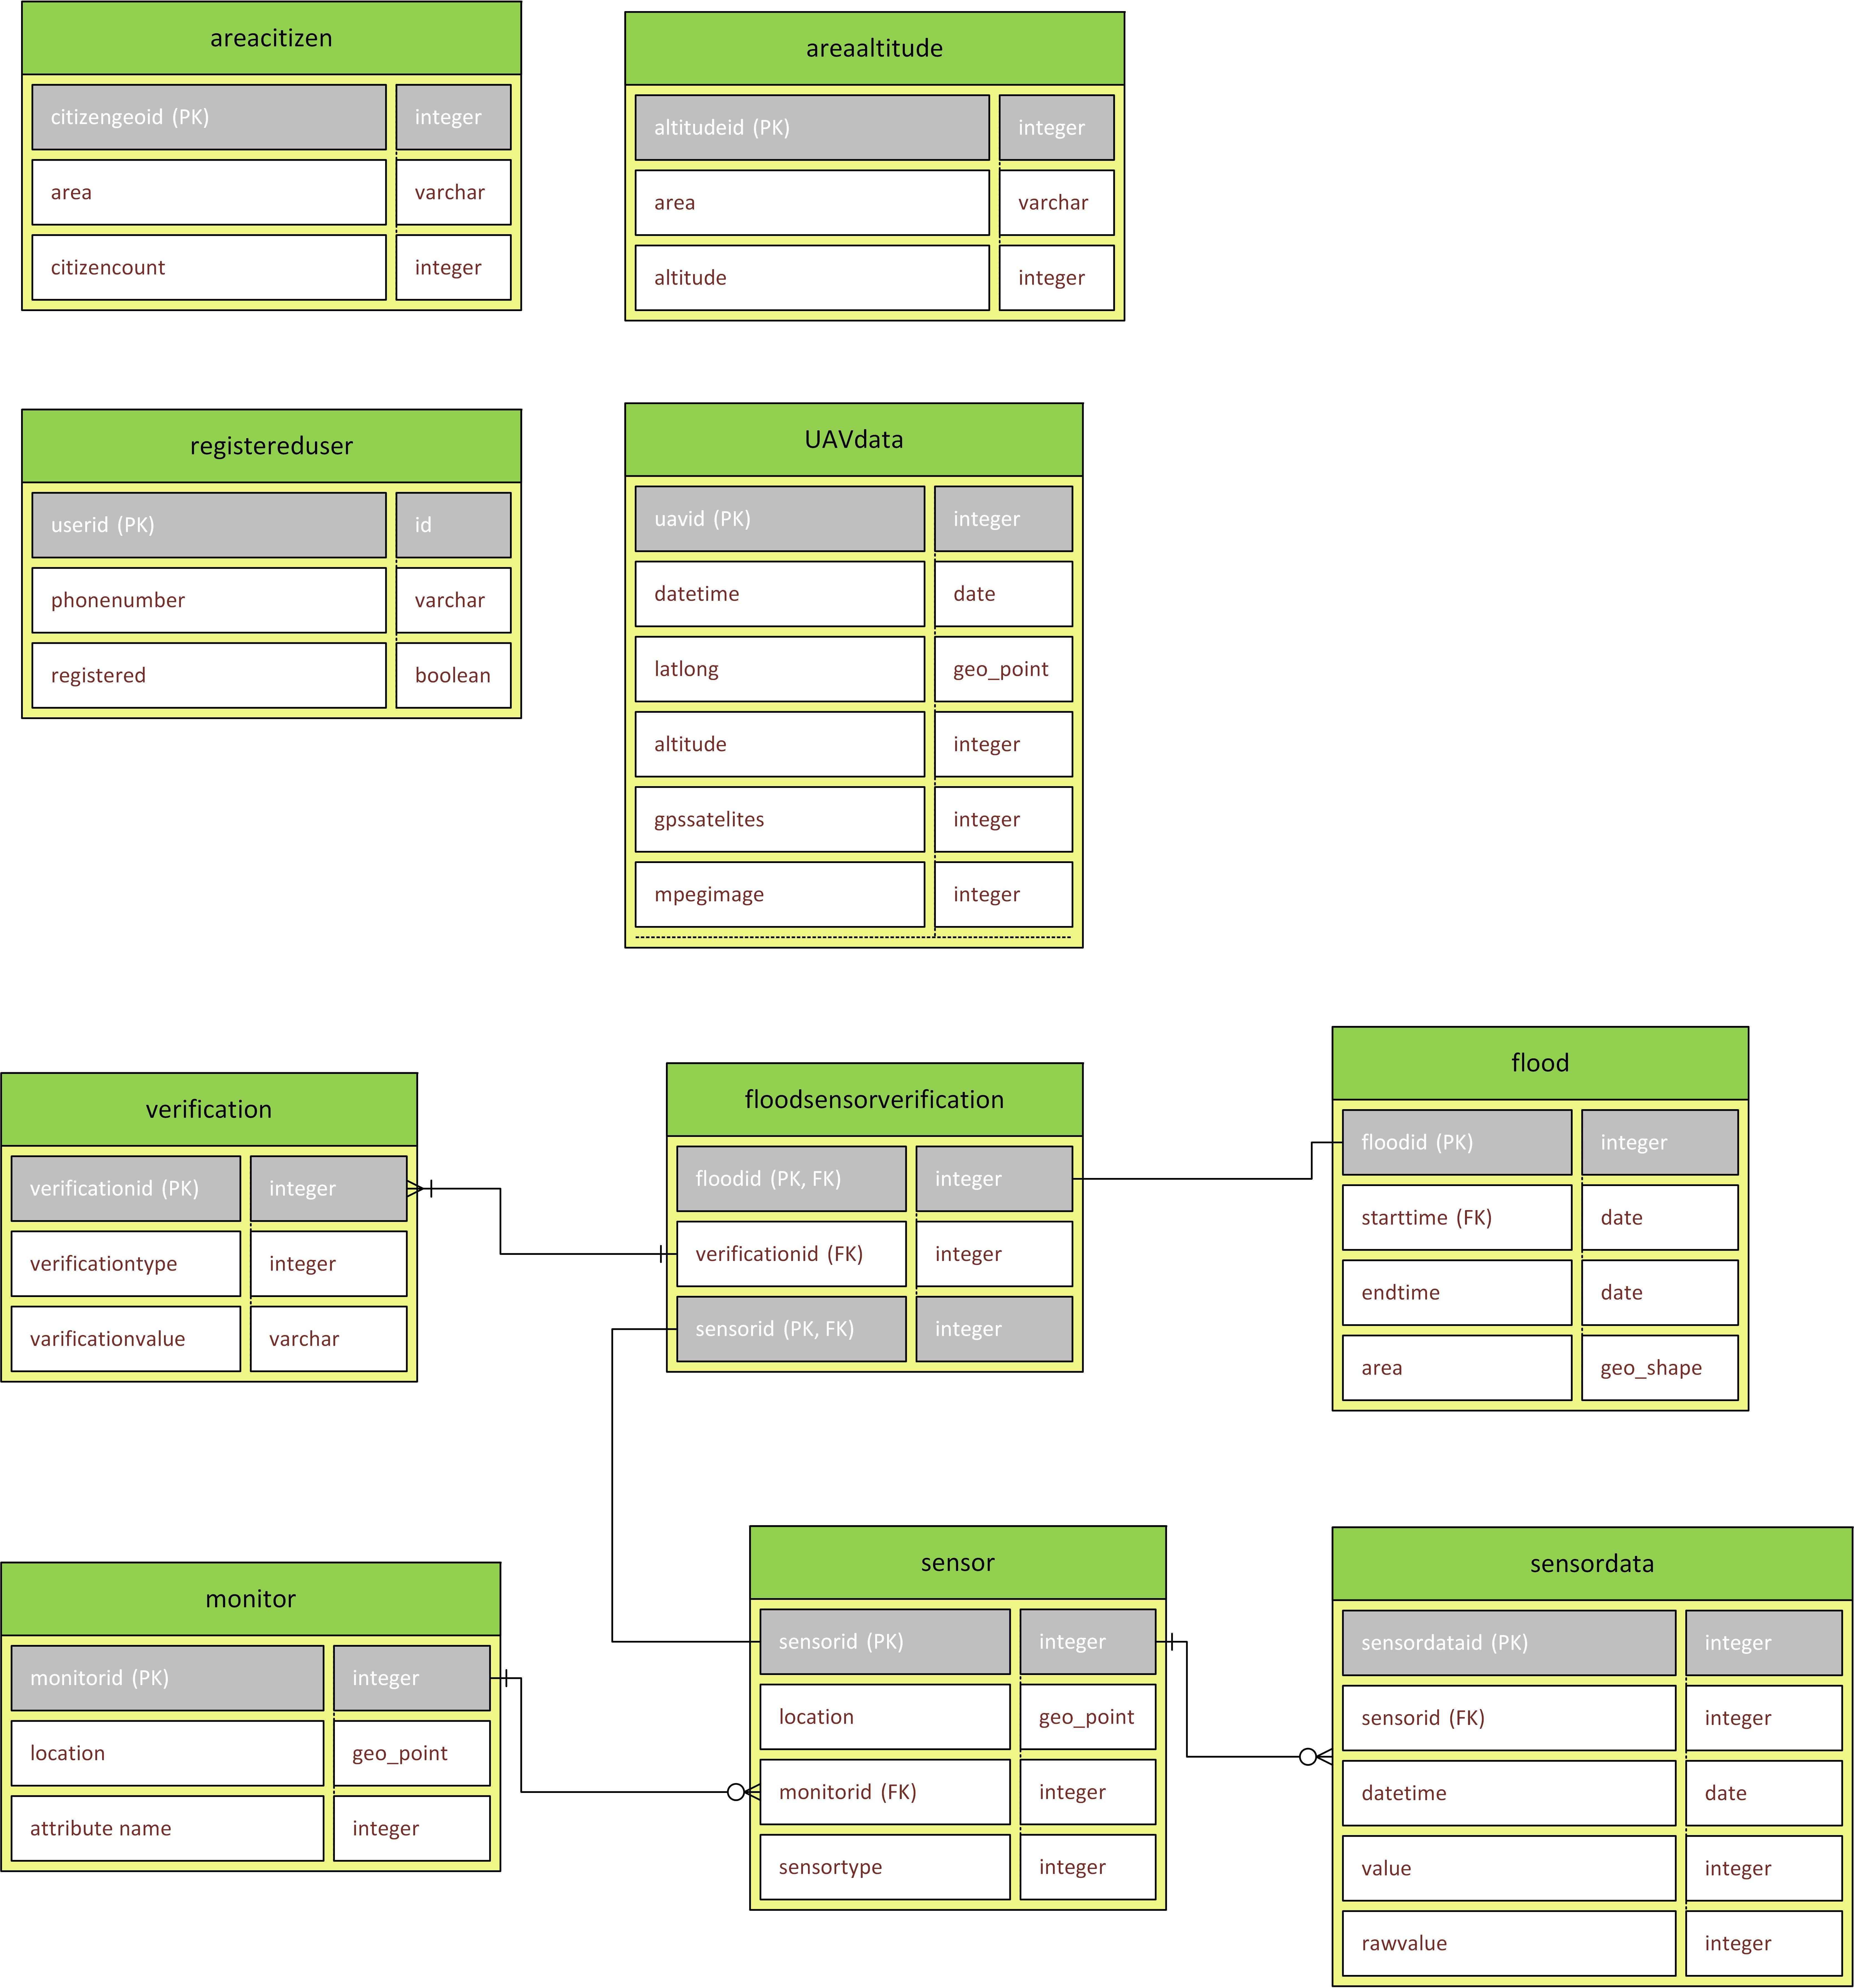
\includegraphics[height=14cm, width=0.9\textwidth]{{\viewimages/database}.jpg}
	\caption{Database diagram}
	\label{fig:database}
\end{figure}

The database diagram shows all the information the API can provide to the users. \\
The database is made of ten tables. \\

In green is the name of the table. \\
In grey the primarykey. \\
In the second column of each table are the types of the data. \\

The first table \textbf{aeracitizen} concerns the area where live the citizens : citizengeold (?) , area : the name of the area and citizencount gives the number of citizen in this area.\\
The table \textbf{aeraaltitude} gives information about the are such as its altitude.
The table \textbf{UAVdata} provides information sent by the UAVs which will give more information about the flood such as : uavid which identifies a specific uav, datetime, altitude , latlong ,gpssatelite,mpegimage, \\
The table \textbf{registereduser} concerns information to identify a specific user to provide him the warning, provide guidance and help the safety region : his id, phonenumer and if he is registered or not. \\

Six table are related and provide information about the sensors : \\
verification (?) \\
The table \textbf{Floodsensorverification} (?) \\
The table \textbf{flood}gives information about the flood : its id by floodid , starttime , endtimide , area. \\
The table \textbf{monitor} : monitorid , its location, attributename. \\
The table \textbf{sensor} : sensorid identifies each sensor, its location , which monitor it depends on,and its type \\
The table \textbf{sensordata} : sensordataid which identifies each data of the sensor, sensorid, datetime which gives the exact time of when the data has been sent ,value,  rawvalue(?). 

\subsubsection{Packages}
The software of the system is divided into several packages. These packages and their relations can be seen in figure~\ref{fig:package-diagram}. 
In this diagram, «use» depicts the use of an interface exposed by a software package, «access» depicts a private import of (parts of) another package, while «import» means a public import of (parts of) another package. 

The diagram contains software packages of the system itself, as well as software packages provided by third parties. The software packages provided by third parties are drawn outside of the `Smart Flood Monitoring System'-box.

The `Third Party API' is the software package which exposes a REST-API, which can be used by third parties to query data from the system.
The `External Data' is the software package which uses APIs from other systems to query data, like weather and geographic data.

\begin{figure}[H]
	%\centering
	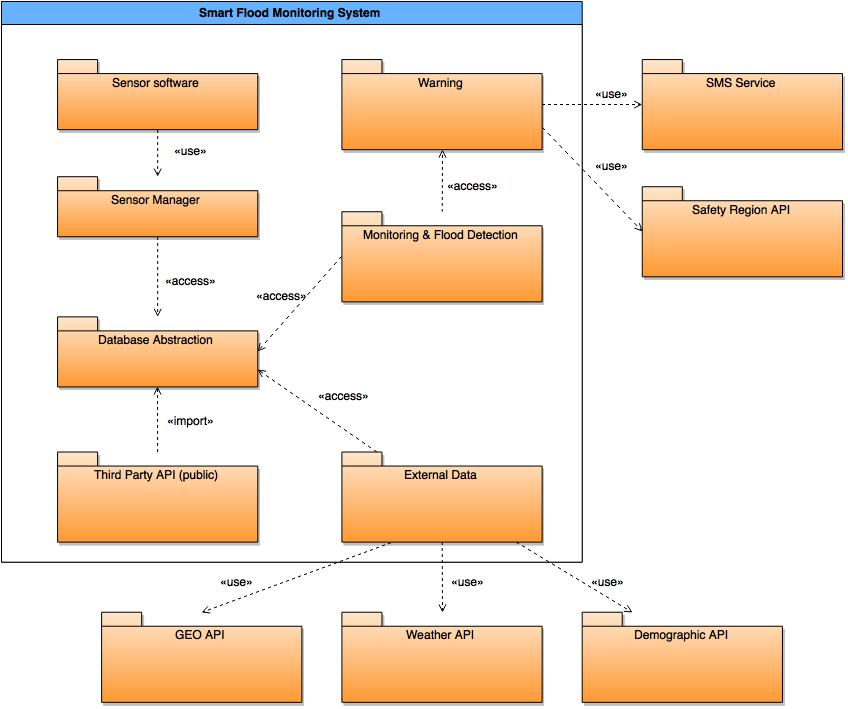
\includegraphics[keepaspectratio=true,width=1.0\textwidth]{{\viewimages/packages}.png}
	\caption{Package diagram}
	\label{fig:package-diagram}
\end{figure}

The following packages are in the system.
	\begin{itemize}
	 \item Sensor Software: This software package is used for retrieving data from the sensors. It uses the sensor manager.
	 \item Sensor Manager: Responsible for installing sensors and configure the sensors.
	 \item Data Abstraction: Holds all data that is stored in the system.
	 \item Third Party API: Package that enables third party software too access data from the system database.
	 \item External Data: This package retrieves data from the GEO API, Weather API and Demographic API.
	 \item Monitoring \& Flood detection: Access the data from database and calculates if a flood is imminent. 
	 \item Warning: When a flood is imminent the warning package is used to send out a warning.
	\end{itemize}

The following external packages are used:
\begin{itemize}
	\item SMS Service: This package is used to let citizen subscribe to the warning services and send out warnings.
	\item Safety region API: When a flood is imminent a warning is send by the system to the safety region API package.
\end{itemize}


\subsection{Process View}

\copied{Process view : The process view deals with the dynamic aspects of the system, explains the system processes and how they communicate, and focuses on the runtime behavior of the system. The process view addresses concurrency, distribution, integrators, performance, and scalability, etc. UML Diagrams to represent process view include the Activity diagram.}
{from wikipedia}
This view mainly discuss about runtime, concurrency, communication, and synchronization of the process running in the system. \\

The program flow and business logic of the system are captured in this section with the aid of several activity diagrams.

\subsubsection*{Flood monitoring}

The activity diagram in figure~\ref{fig:activity-monitoring} shows the flow of the flood monitoring process.


\begin{figure}[h]
\centering
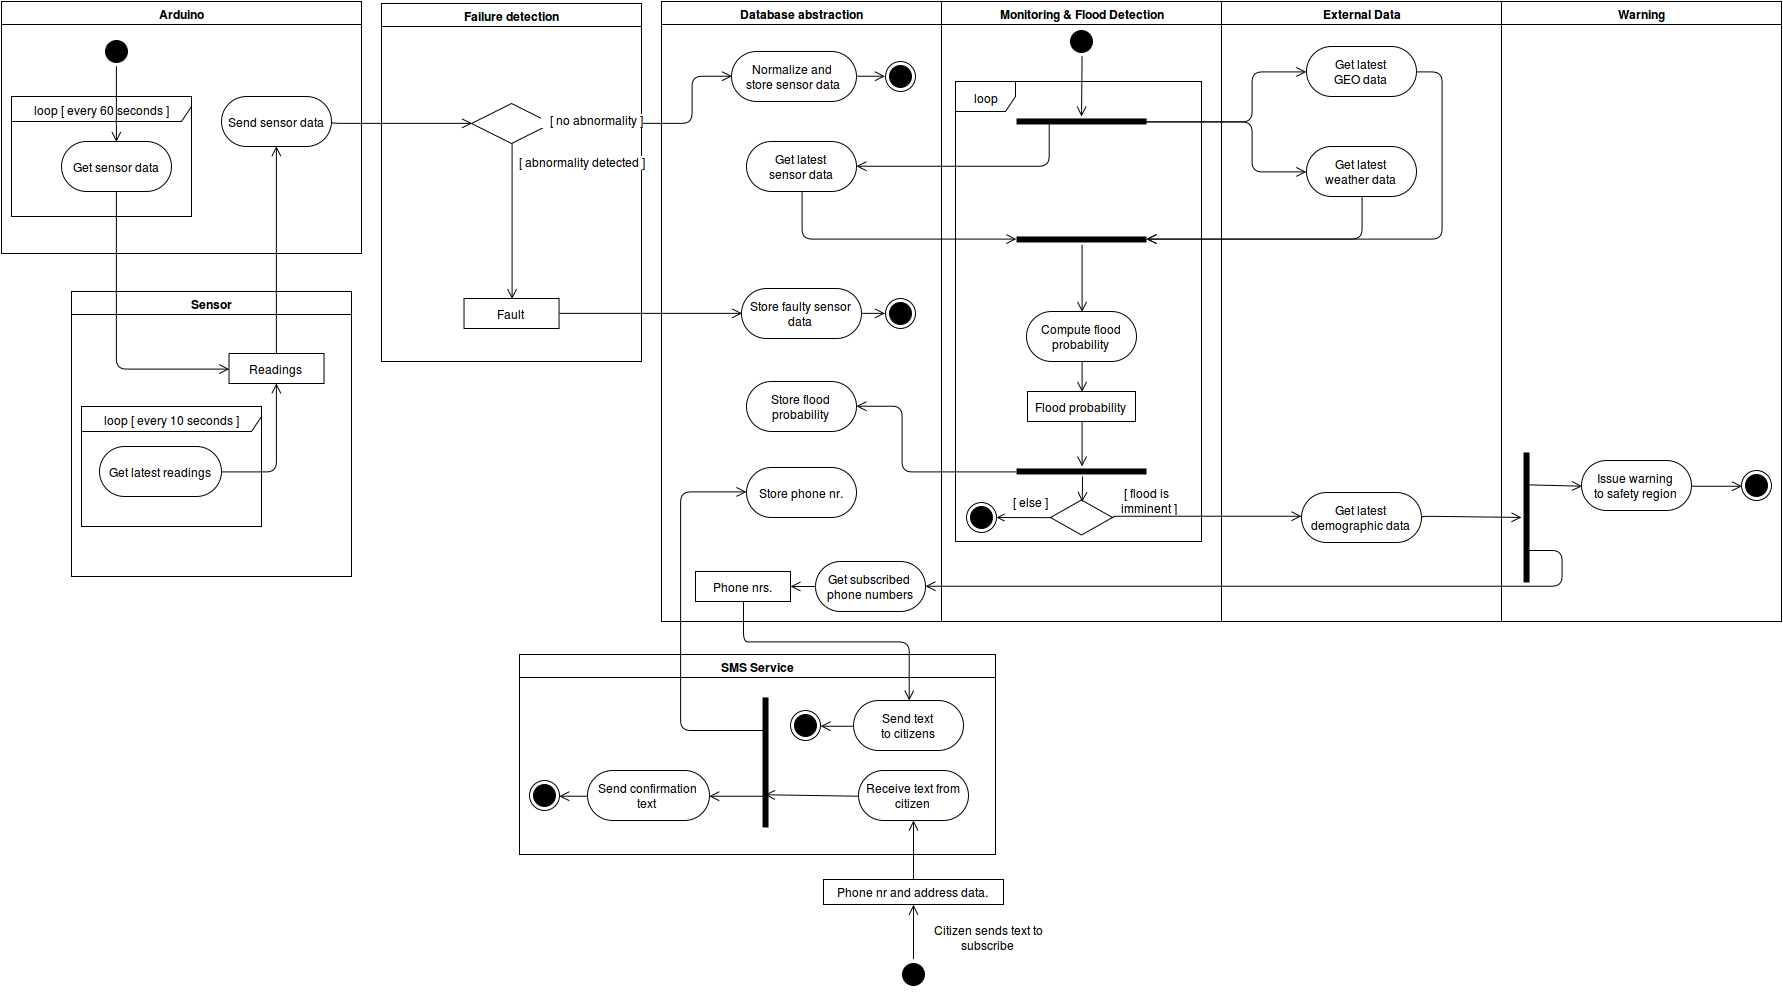
\includegraphics[keepaspectratio=true,width=1.0\textwidth]{{\viewimages/activity_monitoring}.png}
\caption{An activity diagram of the flood monitoring process}
\label{fig:activity-monitoring}
\end{figure}


\subsubsection*{Sending warnings}

In figure~\ref{fig:warning} a sequence diagram of sending warnings to the emergency room and citizens can be seen. The sequence diagram contains a time constraint of 10 seconds and 5 minutes, for warning the emergency room and all citizens respectively.

\begin{figure}[h]
\centering
\includegraphics[keepaspectratio=true,width=1.0\textwidth]{{\viewimages/sequence_warning}.png}
\caption{A sequence diagram of sending warnings to citizens and emergency room}
\label{fig:warning}
\end{figure}


\subsubsection*{Sending the sensor data}
In figure~\ref{fig:sequence-sensordata} a sequence diagram of sending the sensor data can be seen. The sensor has two running threads: one reading the measurements and the other for sending the data every 60 seconds.

\begin{figure}[h]
\centering
\includegraphics[keepaspectratio=true,width=0.7\textwidth]{{\viewimages/sequence_sensor}.png}
\caption{An activity diagram of the flood monitoring process}
\label{fig:sequence-sensordata}
\end{figure}

%!TEX root = ../../report.tex
\clearpage
\subsection{Deployment View}
This subsection outlines the physical arrangement of the nodes in a distributed system, the artifacts that are stored on each node, and the components and other elements that the artifacts implement \cite{ibmdeployment}. Communication paths and deploy relationships model the connections in the system.

\subsubsection{Deployment Diagram}
Figure \ref{fig:deployment-diagram} shows the deployment diagram of the \gls{SFM}. The diagram contains several components such as, sensors, \gls{UAV}, analytics clusters, and database clusters. Main communication between components are done using TCP/IP. All hardware decision are based on chapter 6.
	
% \clearpage

\begin{landscape}
	\begin{figure}[hb!]
	\centering
	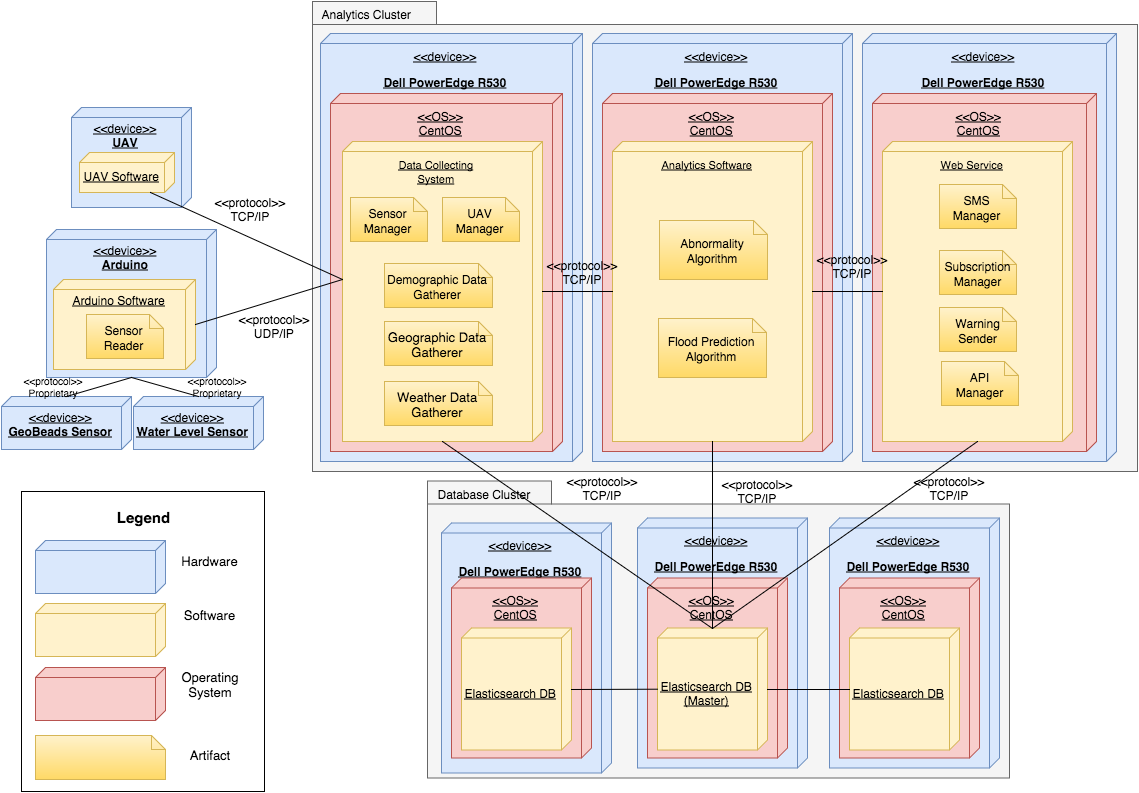
\includegraphics[keepaspectratio=true,width=1.0\textwidth]{{\viewimages/deployment-view}.png}
	\caption{Deployment diagram}
	\label{fig:deployment-diagram}
	\end{figure}
\end{landscape}

% \clearpage

The deployment diagram, depicted in figure \ref{fig:deployment-diagram}, is developed based on \cite{ibmdeployment}. The block with blue color represents hardware components. The red and yellow represent operating system and the SFM developed software. Some artifacts are put inside the software block. Deployment view can be categorized into three main components, such as sensing components, main analytics cluster, and database cluster.

\subsubsection*{Sensing Components}
This portion of the \gls{SFM} is responsible for gathering required data and sending the data to Data Collection System. The \gls{SFM} will utilize two kind of sensor, water level sensor and GeoBeads sensor. Water level sensor is required to measure the water condition of dykes or water ways, while GeoBeads sensor is used to measure the dykes condition. Both kind of the sensor does not have any software part in it as it is merely electronic component that senses the condition of the surroundings. Both of the sensor will be directly connected to Arduino Uno Ethernet. Arduino will pack the data gathered from sensors and periodically send it to the Data Collecting System.

Furthermore, \gls{UAV} will fly if it is necessary. \gls{UAV} will take certain pictures, which is impossible for human to take it, that will be useful for maintenance of the \gls{SFM} or fixing certain problem.

\subsubsection*{Main Analytics Clusters}
Main analytics cluster is responsible for gathering data and storing it to the database, detecting possible faulty sensors, and analyzing the gathered data to predict imminent flood. The main analytics cluster consist of three main components: data collecting system, analytics cluster, and web service that is open to public.

The \gls{SFM} will run three data centers to maintain the key drivers of the system. Two of them will be located inside the Netherlands and one will be located abroad. However, figure \ref{fig:deployment-diagram} only shows one of them for the sake of simplicity.

\subsubsection*{Database Cluster}
This component will store the data coming from sensors and \gls{UAV}. The \gls{SFM} will not store any weather data because the data is always available in the weather provider, thus there is no need to store the data. The \gls{SFM} will run Elasticsearch database because it is suitable for storing data that the \gls{SFM} will have.

\subsubsection{Artifacts}
Figure \ref{fig:deployment-diagram} contains several artifacts that are derived from \autoref{fig:elaborated-model}, \autoref{fig:layers}, \autoref{fig:logical}, \autoref{fig:component}, and \autoref{fig:package-diagram}. Elaboration of the artifacts will also be categorized into two main components: sensing components and main analytics cluster.

\subsubsection*{Sensing Components}
\begin{table}[h!]
\begin{tabular}{L{0.2\textwidth} L{0.6\textwidth}}
    \textbf{Artifact} 		& \textbf{Description} \\ \toprule
    Sensor Reader	 		& Sensor reader is responsible for packing the data gathered from sensor to be ready to be sent.\\ \bottomrule
\end{tabular}
\caption{Artifact for sensing component}
\label{table:sensing-artifacts}
\end{table}

\subsubsection*{Main Analytics Clusters}
% \begin{longtable}[h!]
\begin{longtable}{L{0.2\textwidth} L{0.6\textwidth}}
	\centering
    \textbf{Artifact} 			& \textbf{Description} \\ \toprule
    Sensor Manager				& Sensor manager is responsible for managing input 									coming from multiple sensors (Arduino).\\ \midrule
    \gls{UAV} Manager 			& \gls{UAV} manager is responsible for handling incoming 							 data from \gls{UAV}s.\\ \midrule
    Demographic Data Gatherer	& This is responsible for getting data from demographic 							data provider.\\ \midrule
    Geographic Data Gatherer	& This is responsible for getting data from geographic 								data provider.\\ \midrule
    Weather Data Gatherer		& This is responsible for getting data from weather data 							 provider.\\ \midrule
    Abnormality Algorithm		& Abnormality algorithm is responsible for detecting 								faulty sensors.\\ \midrule
    Flood Prediction Algorithm  & This is the main part of algorithm, which will detect 							imminent flood. \\ \midrule
    SMS manager 				& SMS manager is responsible for handling outgoing SMS 								to certain users.\\ \midrule
    Subscription Manager 		& Subscription manager is responsible for managing 									subscription of citizens/users.\\ \midrule
    Warning Sender				& Warning sender is responsible for sending warnings to 							Safety region.\\ \midrule
    API Manager 				& This is responsible for managing outgoing API to third 							 party developers.\\ \bottomrule
    \caption{Artifact for main analytics cluster}
	\label{table:main-analytics-artifacts}
\end{longtable}

% \end{longtable}


%This is part of the views...?
%Component diagram in the Development view
%https://en.wikipedia.org/wiki/4%2B1_architectural_view_model
%%!TEX root = ../report.tex
\section{Components}
This section outlines the components of the software system, including their functionality, interfaces, and interactions.

%Also part of the views. In the views you discuss the decissions
%!TEX root = ../report.tex
\section{Software design decision}
This section highlights some of the design decisions that have been made, especially those that are not covered in the previous views.

%%%%%%%%%%%%%%%%%%%%%%%%%%%%%%%%%
% DECISIONS TO MAKE
%%%%%%%%%%%%%%%%%%%%%%%%%%%%%%%%
	%Data Mapper for the data layer.
	%alternatives: table data gateway, active record, ...
	
	%Push/pull from sensors: 	Push model reduces the server load. No requests so no high load. No data management, no security management. No DOS. 
	%							Downside: Data will be received that was not requested, even if not interested. 
	%
	%Update monitor system firmware? Is this needed? Do we do this? And how do we do this?
	%Do sensors have firmware and how do we update that?
	%
	%How to controll the uav? Manually or auto pilot? (see Auto flight: (105.pdf p110): 4.3 Manual versus autonomous flight)
	%
	%How to process the uav data. Maybe: Pix4D software automatically processes terrestrial and aerial imagery acquired by light-weight drones or aircraft using its innovative technology based purely on image 	content. This desktop software converts your images into highly precise, timely and customizable results for a wide range of GIS and CAD applications.
	%\url{https://pix4d.com/}
	
	

\pgfplotstabletypeset[%
UCTable
]{%
	value & description \\
	Name & Database \\
	Decision & \req{dec}\\
	Problem/Issue & The system needs a database that \compactList{itemize}{%
			\item Is highly scalable
			\item Has a very good performance
			\item Has a high availability
			\item Has allot of features for storing and querying geospacial data}\\
	Decision & 	\compactCell{The Elasticsearch database is the best database for the SMF system. Elasticsearch is open source, so it will not increase the SMF system costs.  It has native geospacial data / querying support \cite{elasticgeo} and very good geospacial query capabilities \cite{elasticgeoquery}.
				Elasticsearch is extremely distributed and scalable\cite{elasticdistributed}. And Elasticsearch has a very good performance}\\ %\citep{mongovselastic}} \\
%	https://www.elastic.co/products/elasticsearch
%	http://stackoverflow.com/questions/1284083/choosing-a-stand-alone-full-text-search-server-sphinx-or-solr
	Alternatives & PostGreSQL, SQL Server, Oracle, MySQL, SOIR, Sphynx, MongoDB\\
	Arguments & 	\compactCell{%
		\textbf{PostGreSQL} is Opensource and has very good geodata support. However is has no cluster or scalability options, so it has to be hosted on one machine. \\%
		\\%
		\textbf{SQL Server} Has the ability to cluster, but only failover clusters \cite{sqlserverdo}, so no workload balancing. \\
		\\%
		\textbf{Oracle} Has failover clustering options and load balancing options \cite{oracleworkload}, however but costs money.\\
		\\%
		\textbf{MySQL} In previous versions only had support for bounding box capabilities, it had no polygon support \cite{mysqlspacial}. The latest version (Version 5.6.1) does have support for polygons \cite{mysqlspacial}. However, MySQL has not yet proven itself to be very good with spacial data. 
	MySQL can be clustered and load balanced by using other tools \cite{mysqlcluster}.This, however, is a solution that does not provide the scalability the SMF system is looking for. \\
	\\%
	\textbf{SOIR and Sphynx} Are both good choices. Both are able to cluster and distribute and both support geospacial data. However, Elasticsearch scales and distributes better then both \cite{elasticsearchcreator}.\\
	\\
	%http://docs.mongodb.org/manual/applications/geospatial-indexes/
	\textbf{MongoDB} Has every feature the SFM system needs. It provides allot of support for geodata storing and querying. It is also very good in clustering and distributed querying. However, the performance of Elasticsearch is allot better \cite{mongovselastic}.
%	%http://docs.mongodb.org/v2.4/core/sharded-cluster-architectures-production/)
	%However, the performance of elasticsearch is allot better \cite{mongovselastic}.
	}\\
}


% %!TEX root = ../report.tex

\newcommand{\bo}[1]{\textbf{#1}}

\chapter{Architecture evaluation}

\label{ch:evaluation}
In this chapter the software architecture will be evaluated. This document started with a requirement analysis. The requirements which are defined in chapter 3 are checked if they are fulfilled in the software architecture. Another part in this chapter is the architecture evaluation using Architecture Tradeoff Analysis Method (ATAM). The architectural risks can be exposed that can harm the organization's business goals.

\section{Requirements validation}
The requirements from chapter 3 are evaluated in this section. The section is split according to chapter 3. First  the functional requirements, following the commercial requirements, and at the end the technical non-functional requirements.

%!TEX root = ../report.tex

%############################################################
%## FUNCTIONAL 
%############################################################

\subsection{Functional requirements evaluation}

\begin{longtable}{llllL{\tw{0.1}}L{\tw{0.4}}}
    \bo{Nr.} & \bo{Priority} & \bo{Fulfilled} & \bo{Decision} & \bo{Chapter} & \bo{Remarks} \\ \toprule \endhead

    %		INTR-1 & Must     & Yes      &~\ref{subsec:external-system} & Fulfilled by using several weather forecast API providers.       \\ \midrule \midrule
    %The system is able to receive input from water level sensors.
    ~\ref{fr:receive-waterlevel} 
    & Must     
    & Yes
    & ~\ref{hw:1}, ~\ref{hw:2}, ~\ref{hw:3} 
    & ~\ref{sec:hardware-overview},~\ref{subsubsec:components}
    ,~\ref{subsec:logicalview} 
    & Fulfilled by the system providing a REST server the arduino sensor systems can use to post the sensor data to. \\ \midrule

    %The system is able to receive input from the dike sensors.
    ~\ref{fr:receive-pressure}
    & Must
    & Yes
    & ~\ref{hw:2}
    &~\ref{sec:hardware-decisions} ~\ref{hw:2}
    & Fulfilled by having arduino systems sent the dike sensor values over a cabled network to the central system's REST server \\ \midrule

    %The system is able to perform an analysis for the parameters of the dike sensors based on the input from the dike sensors.
    %TODO This has to be explained better i guess.
    ~\ref{fr:analyze-pressure}  
    & Must     
    & Yes        
    & ~\ref{hw:1}
    & ~\ref{subsec:logicalview}, ~\ref{subsec:view-process} 
    & Fulfilled, algorithm uses paramaters of dike sensors. \\ \midrule

    %FR-5 Must The system can store the sensor data.
    ~\ref{fr:store-sensordata}  
    & Must     
    & Yes        
    & ~\ref{dec:6}
    & ~\ref{sec:hardware-overview}, ~\ref{subsec:implementview}, ~\ref{subsec:databaseview}
    & Fulfilled by using an ElasticSearch database that is capable of storing all the data needed.\\ \midrule 

    ~\ref{fr:retrieve-sensordata}
    & Must
    & Yes
    & ~\ref{dec:6}
    & ~\ref{subsec:implementview}, ~\ref{subsec:databaseview}
    &Fulfilled by using an Elasticsearch database that is very robust, high available and scalable. Thereby enhancing the ability to store and receive data at all times. \\ \midrule

    %		%The system retrieves weather forecasting data from weather forecasting services,
    %which consists of predictions about the precipitation, wind data and tide information.
    %This is used by the system to help in determining when a flood becomes imminent
    ~\ref{fr:receive-weather}
    & Must
    & Yes
    & 
    &~\ref{subsec:external-system}
    & Fulfilled by the system contacting several API's to base the decisions on. \\ \midrule 

    %The system is able to detect when a flood is imminent by combining the retrieved
    %sensor data and weather forecasting data.
    ~\ref{fr:detect-flood}
    & Must
    & Yes
    &
    &~\ref{subsec:logicalview}, ~\ref{subsubsec:proc-floodmonitor}
    & Fulfilled by the system using Longitudinal Data Analysis to correlate the sensor data with the forecast data \\ \midrule 

    %		%The system retrieves geographic information, consisting of road data, terrain height
    %data and demographic data (number of civilians living in affected area) from an
    %external API.
    ~\ref{fr:receive-geographic}
    & Must
    & Yes
    &
    &~\ref{subsec:external-system}
    & Fulfilled by the system contacting an external GEO API over TCP/IP\\ \midrule

    %		%The system computes the area affected by a flood, in zones of 5 by 5 km, by using the
    %location data of the sensors and geographic information.
    ~\ref{fr:compute-area}
    & Must
    & Yes
    & ~\ref{dec:6}
    & ~\ref{subsec:database-data},~\ref{subsec:external-system}
    & Fulfilled by the system storing the geographical data in an ElasticSearch database, capable of performing queries to get the specified area \\ \midrule 

    %		%The system is able to perform an analysis, resulting in an estimated expected water
    %level for areas which are affected by a flood, based on the water level sensor data,
    %geographic data and weather forecast information.
    ~\ref{fr:analyze-waterlevel}
    & Must
    & Yes
    &
    &~\ref{sec:elaboratedmodel} ~\ref{subsec:logicalview}
    & Fulfilled by using several different external API's for additional information together with a correlation algorithm and other analysis algorithms \\ \midrule 

    %The system estimates how the water level in the areas affected by the flood will %develop for every hour, up to 12 hours in the future.
    ~\ref{fr:estimate-waterlevel}
    & Should
    & Yes
    &
    & ~\ref{subsec:logicalview}
    & Fulfilled by having the system multiple prediction algorithms to analyze the flood data\\ \midrule 

    %The system can compute the number of civilians living in the areas affected by the flood.
    %TODO: Still no idea what those APIs actually give. 
    ~\ref{fr:compute-nrcivilians}
    & Should
    & Yes
    &
    & ~\ref{subsec:external-system}
    & Fulfilled by letting the system obtain the geo information of the civilians from an external API. Then letting the system store this geo data in the ElasticSearch database, capable of executing complex geo queries. \\ \midrule

    %When a flood is imminent, the system sends a warning to the safety region, containing information about the flood: the area affected by the flood, the expected water level in those areas, how the water level will develop in the coming hours and the number of civilians living in the affected area.
    %TODO explain better in ch7?
    ~\ref{fr:warn-safetyregion}
    & Must
    & Yes
    & ~
    & ~\ref{sec:system-context}, ~\ref{subsec:logicalview}, ~\ref{subsubsec:components}, ~\ref{subsec:view-process}
    & Fulfilled by invoking the emergency room API with a message containing data gathered from the sensor data analysis that led to this warning.\\ \midrule 

    %		\frReqRow{citizens-subscribe}{Must}
    %		{ Citizens are able to subscribe to flood warnings about imminent floods. }	
    ~\ref{fr:citizens-subscribe}
    & Must
    & Yes
    & ~
    & ~\ref{subsec:external-system}, ~\ref{subsec:logicalview}
    & Fulfilled by using an external SMS service provider and providing an API that allows user registration\\ \midrule

    %		\frReqRow{warn-citizens}{Must}
    %		{ Citizens who are subscribed for flood warnings are warned about imminent floods by text message. }
    ~\ref{fr:warn-citizens}
    & Must
    & Yes
    & ~
    & ~\ref{subsec:system-alter}
    & Fulfilled by sending the warning message to the external SMS service provider,  who then distributes it\\ \midrule 

    %		\frReqRow{detect-faultysensor}{Must}
    %		{ The system can detect a faulty sensor, either when the sensor raises an error or when the data from the sensor is inconsistent with other sensor data. }

    %TODO add references:
    %TODO not explained good enough
    ~\ref{fr:detect-faultysensor}
    & Must
    & Yes
    & ~
    & ~\ref{subsec:logicalview}
    & Fulfilled by using algorithms to detect abnormalities and then verifying the abnormalities using the other sensors and algorithms\\ \midrule 

    %TODO way to little in the doc about this
    %		\frReqRow{controlpanel}{Must}
    %		{ There is a control panel, where maintainers of the system have access to. } 
    ~\ref{fr:controlpanel}
    & Must
    & Yes
    & ~
    & ~\ref{subsec:view-process}
    & Fulfilled by allowing maintainers to visit a control panel site that uses the REST interface. \\ \midrule 

    %TODO This control panel is not enough described (and do we still use it?)
    %		\frReqRow{report-faultysensors}{Must}
    %		{ The system reports faulty sensors, so they can be viewed in the control panel. }
    ~\ref{fr:report-faultysensors}
    & Must
    & Yes
    & ~
    & ~\ref{subsec:view-process}
    & Fulfilled by storing abnormal sensor data in a different way in the database, allowing the control panel to distinguishes the faulty sensors \\ \midrule 

    %		\frReqRow{controlpanel-warnings}{Must}
    %		{ Warnings of the system can be viewed in the control panel.}
    ~\ref{fr:controlpanel-warnings}
    & Must
    & Yes
    & ~
    & ~\ref{subsec:view-process}
    & Fulfilled by providing a control panel site the maintainers can visit that shows the warnings that the algorithms stored in the database. \\ \midrule 

    %		\frReqRow{controlpanel-errors}{Must}
    %		{ Errors of the system can be viewed in the control panel. }
    ~\ref{fr:controlpanel-errors}
    & Must
    & ~
    & ~%############################################################
%## Commercial non-functional 
%############################################################
    & ~\ref{subsec:view-process}
    & Fulfilled by providing a control panel site the maintainers can visit that shows the errors that the algorithms stored in the database. \\ \midrule 

    %		\frReqRow{controlpanel-sensors}{Must}
    %		{ The readings of the sensors can be viewed in the control panel. }
    ~\ref{fr:controlpanel-sensors}
    & Must
    & Yes
    & ~
    & ~\ref{subsec:view-process}
    & Fulfilled by providing a control panel site that uses the REST API to get and display the sensor data.\\ \midrule 

    %TODO not explained
    %		Joris: The backups are kind of created by having redundancy
    %		\frReqRow{make-backups}{Must}
    %		{ The system can make backups of its data (configuration data etc.). }
    ~\ref{fr:make-backups}
    & Must
    & Yes
    & ~\ref{dec:7}
    & 
    & Fulfilled by using CentOS as an operating system. This allows the system to be backed up in various ways.\\ \midrule 

    %		\frReqRow{store-backups}{Must}
    %		{ The system can store created backups on a remote location.}
    ~\ref{fr:store-backups}
    & Must
    & Yes
    & ~\ref{dec:7}
    & 
    & Fulfilled by creating backups using rsync \\ \midrule 

    %		\frReqRow{retrieve-backups}{Must}
    %		{ The system can retrieve the backups it previously created.}
    ~\ref{fr:retrieve-backups}
    & Must
    & Yes
    & ~\ref{dec:7}
    & ~
    & Fulfilled by using rsync to backup the system to a accessible location, allowing the system to retrieve the backups\\ \midrule 

    %		\frReqRow{restore-backups}{Must}
    %		{ The system can restore the backups it previously created after retrieving them. }
    ~\ref{fr:restore-backups}
    & Must
    & Yes
    & ~\ref{dec:7}
    & ~
    & Fulfilled by letting the system rsync the backup into the current running system.\\ \midrule 

    %		\frReqRow{expose-api}{Must}
    %		{ The system exposes an API, allowing third parties to develop applications for guidance of the citizens during a flood. }
    ~\ref{fr:expose-api}
    & Must
    & Yes
    & ~\ref{sec:system-context}
    & ~\ref{sec:elaboratedmodel}, ~\ref{subsec:logicalview}, ~\ref{sec:archvision}, ~\ref{subsec:implementview}
    & Fulfilled by hosting a REST sever API\\ \midrule 

    %TODO 	Can it?
    %		\frReqRow{detect-extremephenomena}{Could}
    %		{ The system is able to detect extreme weather phenomena, like storms etc. }
%    ~\ref{fr:detect-extremephenomena}
%    & Could
%    & Partially
%    & ~
%    & ~ 
%    & Partially fulfilled by gathering information from various external weather API's in combination with using a correlation analysis between the sensor values and the external weather data.\\ \midrule

    %TODO explain what algorithms are used?
    %		\frReqRow{uav}{Should}
    %		{ The system processes and stores data collected using a UAV. }	
    ~\ref{fr:uav}
    & Should
    & Yes
    & ~\ref{hw:4}
    & ~\ref{subsec:databaseview}
    & Fulfilled by having a database capable of storing images and geo information\\ \midrule		

    \caption{Evaluation of functional-requirements}
    \label{table:eval-functional-requirements}
\end{longtable}
%\end{longtable}
%\end{adjustbox}



%############################################################
%## Commercial non-functional 
%############################################################

\subsection{Commercial non-functional requirements}

\begin{longtable}{llllL{\tw{0.1}}L{\tw{0.4}}}
    \bo{Nr.} & \bo{Priority} & \bo{Fulfilled} & \bo{Decision} & \bo{Chapter} & \bo{Remarks} \\ \toprule \endhead

    
	1 & 2 & 2 & 4 & 5 & 6 \\
	
	CNF-2 & Must & Yes & 4 & 4,6 & Fulfilled by the tested Geobead sensors quality and reliability in the market. \\
	CNF-3 & Must & Yes & 4 & 2,3,9 & Fulfilled by the table version and the SMF business plan. \\
	
    % %format:
    % ~\ref{} %nr
    % & %priority
    % & %fulfilled
    % & %Decision
    % & %Chapter
    % & %Remarks
    % \\ \midrule

    %	\reqRow{cnfr}{Must}{The system is affordable. The initial price of the system is lower than 95\%\ of the competitors price in the same market.}

    %	\reqRow{cnfr}{Must}{The expected lifetime of the sensors should be at least three years.}
    	
	% \reqRow{cnfr}{}{Must}{The system is extendable. At least four updates/versions of the system will be released.}	

    \caption{Evaluation of non-functional commercial requirements} 
    \label{table:eval-commercialNF-requirements}\\
\end{longtable}

\subsection{Technical non-functional(NF) requirements}
This subsection elaborates about technical non-functional requirements that contain reliability, availability, resilience, performance, interoperability, security, and scalability.

\subsubsection{Reliability}

\begin{longtable}{llllL{\tw{0.1}}L{\tw{0.4}}}
    \bo{Nr.} & \bo{Priority} & \bo{Fulfilled} & \bo{Decision} & \bo{Chapter} & \bo{Remarks} \\ \toprule \endhead

    % %format:
    % ~\ref{} %nr
    % & %priority
    % & %fulfilled
    % & %Decision
    % & %Chapter
    % & %Remarks
    % \\ \midrule

    %	\reqRow{cnfr}{Must}{The system is affordable. The initial price of the system is lower than 95\%\ of the competitors price in the same market.}

    %	\reqRow{cnfr}{Must}{The sensors have a good quality, so they do not have to be replaced often. The expected lifetime of the sensors should be at least three years.}


    %	\reqRow{rel}{Must}{Data from the sensors is sent via a TCP connection} %	
    REL-1 & Must     & ~        & ~ & ~         & ~       \\ \midrule

    %	\reqRow{rel}{Must}{The system must detect if a sensor supplies wrong measurements, which can be caused, e.g. by improper calibration or defects in the sensor.} 
    REL-2 & Must     & Yes      & ~ & ~    ~\ref{subsec:detecting-faulty-sensor}     & Fulfilled, faulty sensor will be detected and later be repaired.       \\ \midrule

    %	\reqRow{rel}{Must}{The system must at no time fail to detect a flood when this flood becomes imminent (\textit{false negative}).}
    REL-3 & Must     & ~        & ~ & ~         & ~       \\ \midrule

    %	\reqRow{rel}{Must}{The system must not detect a flood, when this flood is not there in reality (\textit{false positive}), on average more than once per 5 years.}
    REL-4 & Must     & ~        & ~ & ~         & ~       \\ \midrule
	\caption{Evaluation of non-functional reliability requirements}
    \label{table:eval-technical-nf}\\
\end{longtable}


\subsubsection{Availability}
\begin{longtable}{llllL{\tw{0.1}}L{\tw{0.4}}}
    \bo{Nr.} & \bo{Priority} & \bo{Fulfilled} & \bo{Decision} & \bo{Chapter} & \bo{Remarks} \\ \toprule \endhead

    % %format:
    % ~\ref{} %nr
    % & %priority
    % & %fulfilled
    % & %Decision
    % & %Chapter
    % & %Remarks
    % \\ \midrule
    
%Nr.   & Priority & Fulfilled & Decision & Chapter & Remarks \\ \midrule
%
%        %	\reqRow{ava}{Must}{The system must have an uptime of $99.7\%$. This effectively means, that the system should not be down for more than 2 hours per month.
%        AVA-1 & Must     & Yes      & & ~\ref{subsec:availability}         & Fulfilled.       \\ \midrule
%        %	\reqRow{ava}{Must}{The system must not experience a period of downtime, spanning more than 12 hours. Within twelve hours of the system going offline, it should be back up again. }
%        AVA-2 & Must     & ~        & & ~         & ~       \\ \midrule
%        % \reqRow{ava}{Must}{The system pulls weather forecasts from at least two weather forecasting services.}
%        AVA-3 & Must     & ~        & & ~         & ~       \\ \midrule    
%    
    \caption{Evaluation of non-functional availability requirements} 
    \label{table:eval-functional-requirements}
\end{longtable}

\subsubsection{Resilience}
\begin{longtable}{llllL{\tw{0.1}}L{\tw{0.4}}}
    \bo{Nr.} & \bo{Priority} & \bo{Fulfilled} & \bo{Decision} & \bo{Chapter} & \bo{Remarks} \\ \toprule \endhead

    % %format:
    % ~\ref{} %nr
    % & %priority
    % & %fulfilled
    % & %Decision
    % & %Chapter
    % & %Remarks
    % \\ \midrule

%		Nr.   & Priority & Fulfilled & Decision & Chapter & Remarks \\ \midrule
%
%        %	\reqRow{res}{Must}{The system recognizes failures within half an hour}
%
%        RES-1 & Must     & ~        & ~ & ~         & ~       \\ \midrule
%
%        %	\reqRow{res}{Must}{The system recovers from failures without the \qos or the functionality of the system being affected.} % GK: split in two requirements. reduce to detect sensor failures within half an hour
%
%        RES-2 & Must     & ~        & ~ & ~        & ~       \\ \midrule
%
%        %	\reqRow{res}{Must}{All system data must be backed up every 24 hours, so that in case of data loss, this data can be restored.}
%        RES-3 & Must     & Yes      & ~ & ~\ref{subsec:database-data}         & Fulfilled, the data is also duplicated in database.       \\ \midrule
%
%        %	\reqRow{res}{Must}{In case of a data loss, the data should be retrieved and restored from a backup within 2 hours.}
%        RES-4 & Must     & ~        & ~ & ~         & ~       \\ \midrule
%
%        %	\reqRow{res}{Must}{Backup copies are stored in a secure location which is not in the same area as the system (50 km).}		
%        RES-5 & Must     & Yes      & ~ & ~\ref{sec:hardware-overview}         & Fulfilled, the data centers will be located in three different places.       \\ \midrule

	\caption{Evaluation of non-functional resilience requirements}
    \label{table:eval-technical-nf}\\
\end{longtable}


\subsubsection{Performance}
\begin{longtable}{llllL{\tw{0.1}}L{\tw{0.4}}}
    \bo{Nr.} & \bo{Priority} & \bo{Fulfilled} & \bo{Decision} & \bo{Chapter} & \bo{Remarks} \\ \toprule \endhead

        %	\reqRow{perf}{Must}{Data is transmitted from and to the system with a minimum average speed of 10 megabits per second}
        PERF-1 & Must     & Unknown  & - & -         & Expected, not yet tested. \\ \midrule

        %	\reqRow{perf}{Must}{	The data transmission between the sensors and the system is on average at least 10 megabits per second for each sensor.}
        PERF-2 & Must     & Unknown  & - & -         & Expected, not yet tested. \\ \midrule

        %	\reqRow{perf}{Must}{	The time for the system to compute if there is a flood or not according to a critical level and the data received from the sensors is at most 5 minutes. }
        PERF-3 & Must     & Unknown  & - & -         & Expected, not yet tested. \\ \midrule

        %	\reqRow{perf}{Must}{ If an imminent flood is detected, the warning text message to citizens arrives in 5 minutes. }
        PERF-4 & Must     & Unknown  & - & -         & Expected, not yet tested. \\ \midrule

        %	\reqRow{perf}{Must}{ If an imminent flood is detected, the warning to the emergency room arrives within 1 minute. }
        PERF-5 & Must     & Unknown  & - & -         & Expected, not yet tested. \\ \midrule

	\caption{Evaluation of technical NF-requirements}
    \label{table:eval-technical-nf}\\
    \end{longtable}

\subsubsection{Interoperability}
\begin{longtable}{llllL{\tw{0.1}}L{\tw{0.4}}}
    \bo{Nr.} & \bo{Priority} & \bo{Fulfilled} & \bo{Decision} & \bo{Chapter} & \bo{Remarks} \\ \toprule \endhead

        Nr.    & Priority & Fulfilled & Decision & Chapter & Remarks \\ \midrule
        % \reqRow{intr}{Must}{The system is able to retrieve data from different types of water level sensors and dike sensors. Also future versions of the sensors should be supported.}
        INTR-1 & Must     & Yes      & ~\ref{dec:3} & ~\ref{sec:hardware-overview} & Fulfilled by using GeoBeads and Water level sensor. \\ \midrule
        % \reqRow{intr}{Must}{The system is able to retrieve external data from different weather forecast, demographic and geographic APIs. Also future versions of the APIs should be supported.}
        INTR-2 & Must     & Yes      & &~\ref{subsec:external-system} & Fulfilled by using several external API providers.       \\ \midrule

	\caption{Evaluation of non-functional interoperability requirements}
    \label{table:eval-technical-nf}\\
\end{longtable}
\subsubsection{Security}
\begin{longtable}{llllL{\tw{0.1}}L{\tw{0.4}}}

        Nr.   & Priority & Fulfilled & Decision & Chapter & Remarks \\ \midrule
        % \reqRow{sec}{Must}{Access to the system is restricted to users, which are authorized and authenticated using a password protected user account.}
        SEC-1 & Must     & Yes      & & ~\ref{subsec:system-diagram} & Fulfilled, the user must be authorized to enter the system. \\ \midrule
        % \reqRow{sec}{Must}{All communication to, from and within the system is encrypted.}
        SEC-2 & Must     & Yes      & ~\ref{dec:9} & ~\ref{subsec:channels-information-flows} & Fulfilled, by using secure channel. \\ \midrule
        % \reqRow{sec}{Must}{User account information is stored encrypted.}
        SEC-3 & Must     & Yes      & ~\ref{dec:6} & ~\ref{subsec:database-data} & Fulfilled, applied in Elasticsearch DB. \\ \midrule
        % \reqRow{sec}{Must}{The system is protected on both the application layer and network layer.}
        SEC-4 & Must     & Yes      & & ~\ref{sec:hardware-overview} & Fulfilled, in the data center level. \\ \midrule
        % \reqRow{sec}{Must}{The system communicates with the sensors via a secure HTTPS connection.}
        SEC-5 & Must     & Yes      & ~\ref{dec:9} & ~\ref{sec:hardware-overview} & Fulfilled, by using Arduino to send data. \\ \midrule

	\caption{Evaluation of non-functional security requirements}
    \label{table:eval-technical-nf}\\
\end{longtable}

\subsubsection{Scalability}
\begin{longtable}{llllL{\tw{0.1}}L{\tw{0.4}}}
        Nr.     & Priority & Fulfilled & Decision & Chapter & Remarks \\ \midrule
        % \reqRow{scale}{Must}{The database and services of the system can scale within 1 hour, when the systems resource usage increases.}
        SCALE-1 & Must     & Yes      & ~\ref{dec:6} & ~\ref{subsec:database-data} & Fulfilled by adapting Elasticsearch. \\ \midrule
        % \reqRow{scale}{Must}{The system is configurable to run in different areas and with different sensors.}
        SCALE-2 & Must     & Yes      & & ~\ref{sec:hardware-overview} & Fulfilled by adapting multiple data centers and multiple sensor type. \\ \midrule
        % \reqRow{scale}{Must}{The system maintains the performance requirements when the number of sensors is increased and the data from sensors is expanded.}
        SCALE-3 & Must     & Unknown  & & -         & Expected, not yet tested. \\ \midrule

	\caption{Evaluation of non-functional scalability requirements}
    \label{table:eval-technical-nf}\\
\end{longtable}


\clearpage
% !TEX root = ../report.tex
\section{Architecture evaluation}
The architecture that is shown in the previous chapters needs to be evaluated. This is done with the ATAM method. ATAM stands for Architecture Trade-off Analysis Method. This evaluation method is used to determine if the system meets the requirements that are composed in chapter 3. ATAM identifies critical design decisions and verifies them againts our key drivers. If the design decisions do not fulfill the key drivers, risks for the system will be inevitable. In order to terminate these risks, solutions are provided to deal with the risks. In the remainder of this chapter the architectural approaches, utility tree and the scenarios are provided. 


% The ATAM method is used to evaluate the software architecture. The purpose of ATAM is elicit and refine a precise statement of the architecture’s driving quality attribute requirements\\
% • elicit and refine a precise statement of the architectural design decisions \\
% • evaluate the architectural design decisions to determine if they satisfactorily address the
% quality requirements [add source]
% %/ source: Using the Architecture Tradeoff Analysis Method to Evaluate a Wargame Simulation System: A Case Study Lawrence G. Jones Anthony J. Lattanze December 2001 Architecture Tradeoff Analysis Initiative 

% The method consists of the following steps:[add source] \\
% 1. Present the ATAM: The evaluation team presents a quick overview of the ATAM steps,
% techniques used, and outputs from the process. \\
% 2. Present the business drivers: The system manager briefly presents the business drivers
% and context for the architecture. \\
% 3. Present the architecture: The architect presents an overview of the architecture.
% 4. Identify architectural approaches: Itemize the architectural decisions discovered in the
% previous step.\\
% 5. Generate the quality attribute utility tree: Identify, prioritize, and refine the most
% important quality attribute goals in a utility tree format.\\
% 6. Analyze architectural approaches: Probe the architectural approaches in light of the
% quality attributes in order to identify risks, sensitivity points, and tradeoffs.\\
% 7. Brainstorm and prioritize scenarios: Create and analyze scenarios that represent the
% various stakeholders’ interests to understand quality attribute requirements and their
% relative importance.\\
% 8. Analyze architectural approaches: Continue to identify risks, sensitivity points, and
% tradeoffs while noting the impact of each scenario on the architectural approaches. \\
% 9. Present results: Recapitulate the ATAM steps, outputs, and recommendations. \\
% %/ source: Using the Architecture Tradeoff Analysis Method to Evaluate a Wargame Simulation System: A Case Study Lawrence G. Jones Anthony J. Lattanze December 2001 Architecture Tradeoff Analysis Initiative 

% The first three steps are presented in the previous chapters. In this sub-chapter the focus will be on step 4 and further. 

\subsection{Architectural approaches}
This section lists the architectural approaches used in the document.
The most important part of our system is to warn people in case of a flood. The decision was made to warn citizens through SMS. This solution is available for all mobile phones and can used without the use of internet. It is the most reliable solution to warn citizens. To warn the safety region, the decision was made to use the emergency room API. This API is able to receive warnings and updates from our system. 

Another major design decision was how to connect the different sensors to the system. The decision was made to use a wired connection between the sensors and the hubs. A wireless protocol wouldn't suffice, since the signal isn't strong enough to go through dikes. Connecting sensors to the hubs in this way, makes it also easier to power the sensors. A power wire can simply be added, instead of using batteries or solar panels. The decision to use hubs was made to make the system more structured and organised. Hubs can send data to the central system, this means the system doesn't get to much connections. 

Citizens want to get proper guidance in case of a flood. Third party developers will develop this feature. In order to make this happen the system provides data to the third party developers. The decision to let third party developers develop this application was chosen over developing such a feature ourselves. This was done to keep the focus fully at designing a good architecture for the most important part, the flood detecting and warning system. This decision also gives the possibility for other developers to use our data and create creative applications. 

In the software architecture, the layer pattern is used to seperate the functionality of the system. This is implemented to make the system more reliable, maintainable and extendable.

Short summary of the most important decisions:
\begin{itemize}
	\item Send warnings by SMS to citizens
	\item Use the emergency room API to warn the safety region
	\item Use hubs to connect the sensors to the system
	\item Connect sensors through wires to the hubs
	\item Allow third party developers to create a guidance application
	\item Use the layer pattern in the software architecture
\end{itemize}


\subsection{Quality attribute utility tree approaches}
The utility tree is one of the ATAM techniques it represents the overall usefulness of the system. 
In this section the utility tree is built according to the key drivers of our system : reliability, performance and availability ( view part 3.3 ). The purpose of the utility tree is to elect high priority scenarios which will be analysed precisely in the next section.
The scenarios serve as the leafs of the utility tree and the architecture is evaluated by considering how it makes the scenarios possible. \\


There are four levels in the three . The first node is the root : " Utility " , then follow the Quality factors wich are our key drivers , then the tree goes deeper in precison with refined the key drivers in subfactors which are demonstrated by the leaves with the scenarios we expect our system to manifest. \\

In order to prioritize the scenarios two criterias are used and classified as follow: \\
\textit{Importance  to system success}: High (Very important feature for the system : essential), Medium, Low (Not mandatory)\\
\textit{ Risk/difficulty in achieving}: High, Medium, Low\\
To get the meaning of High , Medium and Low we can use a scale from 10 to 0 as reference: High : 10-7, Medium 6-4, Low 4-0.

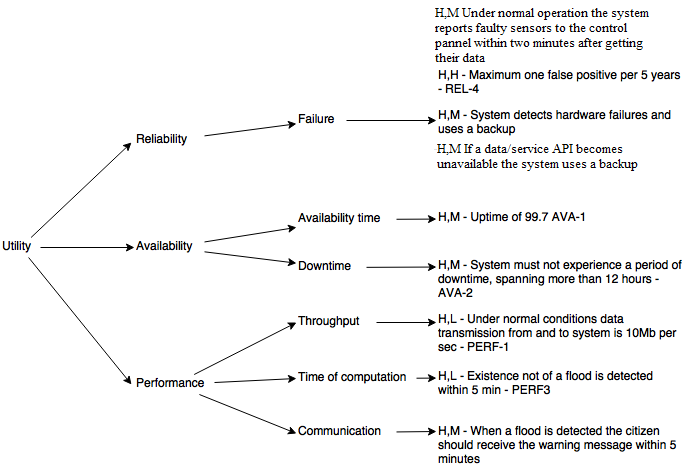
\includegraphics[scale=0.5]{images/utilitytree1.png}

The interesting scenarios are the ones with high priority (H,H),(H,M) and (M,H), focus will be put on them in the next section.
%Using this table we can give points to those scenarios.

\subsection{Scenarios}

In this part high priority scenarios derived from the utility tree will be analysed and as a result will come the identification of sensitivity points, tradeoffs, risks and non risks.


\begin{table}[H]
	\begin{tabular}{L{0.2\textwidth} L{0.6\textwidth}}
		\textbf{Scenario}		& \textbf{Handling faulty sensors} \\ \toprule
		\textbf{Q-Attribute(s)} & Availability, reliability \\ \midrule
		\textbf{Environment} 	& Normal operation \\ \midrule
		\textbf{Stimulus} 		& A sensor sends wrong data or stops sending data \\ \midrule
		\textbf{Response} 		& The system ignores the sensor until is has been repaired/replaced \\ \midrule
		\textbf{Design decisions} 	& \\
			\multicolumn{2}{c}{
			\begin{tabular}{l|lllll}
				\textbf{Decision} & Req. & Sensitiv. & Tradeoff & Risk & Non-Risk \\ \hline
				
				Detection algorithm & \ref{fr:detect-faultysensor}, \ref{rel:2} & \nsl{s}{faultysensor} & \nsl{to}{faultysensor} &  &   \\
				Reporting & \ref{fr:report-faultysensors} &  &  & \nsl{r}{reportfaultysensor} &  \\
				UAV & \ref{fr:uav} & \nsl{s}{uav} & \nsl{to}{uav} & \nsl{r}{uav-weather} & \\
				
			\end{tabular} 
			} \\
			\midrule
			\multicolumn{2}{c}{\compactCell{
				\textbf{Sensitivities:} 
				\begin{itemize} \setlength{\itemsep}{-15pt}
				\item \ref{s:faultysensor}: Some of the time, it will be difficult for the detection algorithm to distinguish between extreme data from a sensor caused by a fault and extreme data caused by a flood.\\
				\item \ref{s:uav}: It takes time for the UAV to be dispatched to the potential flood location.
				\end{itemize} ~\\[-0.5cm]
				\textbf{Tradeoffs:} 
				\begin{itemize} \setlength{\itemsep}{-15pt}
				\item \ref{to:faultysensor}: Reliability (+) vs. Performance (-) -- Using an algorithm on the sensor data to detect faulty sensors adds more overhead, but increases the reliability of the system.\\
				\item \ref{to:uav}: Reliability (+) vs. Performance (-) -- The UAV checks if a flood is present/developing when the sensor data is not conclusive. It has a large dispatch time, which means (if there is a flood), it will be detected with a larger delay. 
				\end{itemize} ~\\[-0.5cm]
				\textbf{Risks:} 
				\begin{itemize} \setlength{\itemsep}{-15pt}
				\item \ref{r:reportfaultysensor}: There is a risk that the config panel where the faulty sensors are reported, is not checked often enough, leading to broken sensors not being replaced.
				\end{itemize}
			}} \\

		\midrule
		\textbf{Reasoning} 		& Temporarily ignoring faulty sensors allows the system to continue functioning. Reporting the sensors using the control panel allows maintenance personnel to repair those sensors. It is important that maintenance personnel checks the control panel regularly. 
		
		In case it cannot be determined by the system if a sensor is faulty, or whether there is a flood, a UAV can be dispatched to check. \\
		%\midrule
		%\textbf{Arch. model} 	&  \\
								 
	 \bottomrule
	\end{tabular}
	\label{ATAM:faulty-sensors}
	\caption{ATAM -- Handling faulty sensors}
\end{table}

\begin{table}[H]
	\begin{tabular}{L{0.2\textwidth} L{0.6\textwidth}}
		\textbf{Scenario}		& \textbf{Handling hardware failures} \\ \toprule
		\textbf{Q-Attribute(s)} & Availability \\ \midrule
		\textbf{Environment} 	& Normal operation \\ \midrule
		\textbf{Stimulus} 		& A hardware component stops operating \\ \midrule
		\textbf{Response} 		& The system uses a backup of the hardware component \\ \midrule
		\textbf{Design decisions} 	& \\
			\multicolumn{2}{c}{
			\begin{tabular}{l|lllll}
				\textbf{Decision} & Req. & Sensitiv. & Tradeoff & Risk & Non-Risk \\ \hline
				
				Database cluster & \ref{ava:1}, \ref{ava:2} &  & \nsl{to}{cluster} &  &   \\
				Analytic cluster & \ref{ava:1}, \ref{ava:2} &  & \ref{to:cluster} &  &  \\
				Multiple data centers & \ref{ava:1}, \ref{ava:2} &  & \nsl{to}{datacentre} &  & \nsl{nr}{datacenters} \\
				Arduino               & \ref{ava:1}, \ref{ava:2} & \nsl{s}{arduinofail} &  &  &  \\
				
			\end{tabular} 
			} \\
			\midrule
			\multicolumn{2}{c}{\compactCell{
				\textbf{Sensitivities:} 
				\begin{itemize} \setlength{\itemsep}{-15pt}
				\item \ref{s:arduinofail}: The Arduino are hardware components which can fail as well. Several sensors are connected to a single Arduino. Since a failing Arduino does not have a backup, those sensors connected to it will become unavailable to the system until the Arduino is repaired. \\
				\end{itemize} ~\\[-1.0cm]
				\textbf{Tradeoffs:} 
				\begin{itemize} \setlength{\itemsep}{-15pt}
				\item \ref{to:cluster}: Availability (+) vs. Affordability (-) -- Using a cluster is more expensive, but provides a fallback in case of failures, increasing the availability. \\
				\item \ref{to:datacentre}: Also Availability (+) vs Affordability (-) -- The costs of the system increase significantly by having a second data center. However, this guarantees the availability of the system in case of problems with one of the data centers.
				\end{itemize} ~\\[-0.5cm]
				\textbf{Nonrisks:} 
				\begin{itemize} \setlength{\itemsep}{-15pt}
				\item \ref{nr:datacenters}: Multiple data centers aid with increasing the availability only when they are not placed in close proximity to each other.
				\end{itemize}
			}} \\

		\midrule
		\textbf{Reasoning} 		& The hardware in the data centers and the data center itself are prepared for failures of components. It is important to note that the data centers should not be placed in close proximity to each other. 
		
		A failure of an Arduino will lead to several sensors going offline, but these sensor are located in a relatively small area and therefore only have a limited impact on the systems monitoring capabilities. \\
		\midrule
		\textbf{Arch. model} 	& See figure~\ref{fig:database-cluster} and figure~\ref{fig:analytic-cluster} for the logical schematic of the database and analytic cluster respectively.
		
		Also see figure~\ref{fig:hardware-archi-schema} for an overview of the multiple data centers. \\
								 
	 \bottomrule
	\end{tabular}
	\caption{ATAM -- Handling hardware failures}
	\label{ATAM:hardware-failure}
\end{table}

\begin{table}[H]
	\begin{tabular}{L{0.2\textwidth} L{0.6\textwidth}}
		\textbf{Scenario}		& \textbf{Ensuring availability of third party data / services} \\ \toprule
		\textbf{Q-Attribute(s)} & Availability, reliability, interoperability \\ \midrule
		\textbf{Environment} 	& Normal operation \\ \midrule
		\textbf{Stimulus} 		& A third party service or data API becomes unavailable \\ \midrule
		\textbf{Response} 		& The system still has access to (a backup of) the data or service \\ \midrule
		\textbf{Design decisions} 	& \\
			\multicolumn{2}{c}{
			\begin{tabular}{l|lllll}
				\textbf{Decision} & Req. & Sensitiv. & Tradeoff & Risk & Non-Risk \\ \hline
				
				Using multiple API providers offering same service/data & \ref{fr:receive-weather}, \ref{fr:receive-geographic} &  & \nsl{to}{apis} &  &   \\
				SMS service & \ref{fr:warn-citizens}, \ref{fr:citizens-subscribe} & \nsl{s}{onesmsservice} &  &  & \nsl{nr}{storingphonenrs}  \\
				Emergency room API & \ref{fr:warn-safetyregion} &  &  &  &  \nsl{nr}{emergencyroomapi} \\
				
				
			\end{tabular} 
			} \\
			\midrule
			\multicolumn{2}{c}{\compactCell{
				\textbf{Sensitivities:} 
				\begin{itemize} \setlength{\itemsep}{-15pt}
				\item \ref{s:onesmsservice}: The system relies on a single SMS Service provider (CM Telecom). If this provider is not available, the system cannot warn citizens by text message. \\
				\end{itemize} ~\\[-1.0cm]
				\textbf{Tradeoffs:} 
				\begin{itemize} \setlength{\itemsep}{-15pt}
				\item \ref{to:apis}: Reliability (+) vs. Affordability (-) -- Most APIs charge a usage fee, which means that using multiple APIs increases the costs. \\
				\end{itemize} ~\\[-1.0cm]
				\textbf{Nonrisks:} 
				\begin{itemize} \setlength{\itemsep}{-15pt}
				\item \ref{nr:storingphonenrs}: The phone numbers of citizens who subscribed are stored in the database of the system instead of the SMS Service provider's database. \\
				\item \ref{nr:emergencyroomapi}: It is assumed that the emergency room API is always available, which is the responsibility of the safety region.
				\end{itemize}
			}} \\

		\midrule
		\textbf{Reasoning} 		& \compactCell{
			By using multiple APIs for weather / geographic / demographic data, it is ensured that this data is available if one of the APIs goes offline. 
			
			The SMS service is a single point of failure: if it goes offline, there is no backup SMS service provider.
		} \\
		%\midrule
		%\textbf{Arch. model} 	& \\
								 
	 \bottomrule
	\end{tabular}
	\caption{ATAM -- Ensuring availability of third party data / services}
	\label{ATAM:3rdpartydata}
\end{table}


%!TEX root = ../report.tex
\chapter{System evolution}
\label{ch:evolution}

\section{Other countries}

\section{Third party guidance evolution}
	- Maybe make our own

\section{UAV evolution}

\section{Satellite}

\section{Other disasters}

\section{Versions}

UAV can spot citizens in need (maybe based on their mobile phone)





%!TEX root = ../report.tex
%\cleardoublepage
%\clearpage
%
%\appendix
%\appendixpage
%\addappheadtotoc

\begin{appendices}

%\addcontentsline{toc}{part}{\appendixname}
	
	\renewcommand{\thechapter}{\Alph{chapter}}
	\renewcommand{\thesection}{\thechapter.\arabic{section}}
	\renewcommand{\thesubsection}{\thesection.\arabic{subsection}}
	\renewcommand{\thesubsubsection}{\thesubsection.\arabic{subsubsection}}

	%!TEX root = ../report.tex
\chapter{Time Tracking}
\label{App: Time Tracking}

%\section{Week #}
%\begin{tabular}{p{0.2\textwidth} p{0.7\textwidth} p{0.1\textwidth}}
%    \textbf{Person} & \textbf{Task} & \textbf{Hours} \\ \midrule
%	Eedema &  &  \\ \midrule
%	Putra &  &  \\ \midrule
%	Fakambi & & \\ \midrule
%	Schaefers &  & \\ \midrule
%	Brandsma &  & \\ \midrule
%	Menninga &  &  \\ \midrule
%\end{tabular}

\section{Week 1}
\begin{tabular}{L{0.2\textwidth} L{0.7\textwidth} L{0.1\textwidth}}
    \textbf{Person} & \textbf{Task} & \textbf{Hours} \\ \toprule
	Eedema & Reviewing the document, reading the assignment, initializing requirements, \& installing environment for project & 8 \\ \midrule
	Putra & Initial preparation for the course & 5 \\ \midrule
	Fakambi & Reading the document and assignment, Preparation and drafts with ideas & 5 \\ \midrule
	Schaefers & Setting up the working environment, create the context page and analysis page drafts. Setting up and improving the the document structure. & 8\\ \midrule
	Klinkenberg & & \\ \midrule
	Brandsma & Creating working environment, reading assignment, first draft business part & 8\\ \midrule
	Menninga & Reading assignment, setting up working environment, first non-functional requirements & 5 \\ \bottomrule
\end{tabular}

\section{Week 2}
\begin{tabular}{L{0.2\textwidth} L{0.7\textwidth} L{0.1\textwidth}}
    \textbf{Person} & \textbf{Task} & \textbf{Hours} \\ \toprule
	Eedema & Coaching session, project planning session and work on business information chapters & 9  \\ \midrule
	Putra & Coaching session, project planning session, project meeting, first version of stakeholder part of requirements & 7.5 \\ \midrule
	Fakambi & Coaching session , project meeting, work on Non functional requirements & 7 \\ \midrule
	Schaefers & First coaching session, improved and enhanced the context and business information chapters. Also created a quality attributes prioritization table.& 8 \\ \midrule
	Klinkenberg & Coaching session, meetings, providing feedback on requirements & 5.5\\ \midrule
	Brandsma & First version of use-cases, coaching session, meeting, use-cases, architectural vision & 6.5 \\ \midrule
	Menninga & First version of the functional requirements, coaching session, meeting & 10.25 \\ \bottomrule
\end{tabular}

\section{Week 3}
\begin{tabular}{p{0.2\textwidth} p{0.7\textwidth} p{0.1\textwidth}}
   \textbf{Person} & \textbf{Task} & \textbf{Hours} \\ \midrule
	Eedema &  Coaching, meetings, analysis, business part, reviewing & 14  \\ \midrule
	Putra & Coaching session, meetings, proofread on chapter 1 and 2, revising stakeholders, database decision part of analysis, and preparing \LaTeX{} file for the presentation & 10 \\ \midrule
	Fakambi & Coaching session, meetings, Non functional requirements and Risk assessment & 10.5\\ \midrule
	Schaefers & Coaching session, meetings, reviewing, Business section & 12 \\ \midrule
	Klinkenberg & Coaching session, meetings, technical requirements, analysis, reviewing & 13.5 \\ \midrule
	Brandsma & Coaching session, meeting, architectural vision, use-cases, analysis & 9 \\ \midrule
	Menninga & Coaching session, meetings, updates functional requirements, reviewing entire document, updated assumptions and some improvements to structure of analysis, added decision about type of water level sensor. & 14.0 \\ \midrule
\end{tabular}

\section{Week 4}
\begin{tabular}{p{0.2\textwidth} p{0.7\textwidth} p{0.1\textwidth}}
   \textbf{Person} & \textbf{Task} & \textbf{Hours} \\ \midrule
	Eedema & Coaching session, meetings, business chapter, review 3, presentations, peer review &13  \\ \midrule
	Putra & Coaching session, meetings, presentation prep., improving business rationale, review chapter 2, making draft of chapter 5, 6, and 7 & 14 \\ \midrule
	Fakambi & Coaching session , meetings , Work on and improvements chapter 3.5 to 3.8 & 12 \\ \midrule
	Schaefers & Researched on sensors and other EWS's. Then created the system architecture model diagram and vision diagram for the presentation I had to present in. Created/improved other diagrams. Researched about the costs of these kinds of systems and created/enhanced the business cost section. & 20 \\ \midrule
	Brandsma & Coaching session, meetings , reviewing group 1, architectural vision, use-cases, reviewing, improving chapter 4 & 16.5\\ \midrule
	Menninga & Coaching session, presentation prep., meeting, improvements FR and risks, review ch. 4, improvements to NFR and Risk Assessment & 14.0 \\ \midrule
\end{tabular}

\section{Week 5}
\begin{tabular}{p{0.2\textwidth} p{0.7\textwidth} p{0.1\textwidth}}
    \textbf{Person} & \textbf{Task} & \textbf{Hours} \\ \midrule
	Eedema & Coaching meetings, reviewing, chpt 5  & 13 \\ \midrule
	Putra & Coaching session, meetings, reviewing, working on initial work on chapter hardware, researching on servers, and working on server selection  & 15 \\ \midrule
	Fakambi & Coaching session, meetings, Work on chapter 6 Hardware architecture, drafts, design decision about UAVs & 12.0 \\ \midrule
	Schaefers & Created initial layer diagram, component diagram, sequense diagram and database design diagram. Researched and explained what new database to use.  & 15\\ \midrule
	Brandsma & Coaching session, meetings, chapter 5  & 13 \\ \midrule
	Menninga & Coaching session, meeting Tuesday, lots of improvements to chapter 3, expanding chapter 6 & 15.5 \\ \midrule
\end{tabular}

\section{Week 6}
\begin{tabular}{p{0.2\textwidth} p{0.7\textwidth} p{0.1\textwidth}}
    \textbf{Person} & \textbf{Task} & \textbf{Hours} \\ \midrule
	Eedema & Coaching, meetings, review, system overview, evaluation & 15 \\ \midrule
	Putra & Coaching session, meetings, reviews, hardware overview, deployment view & 13 \\ \midrule
	Fakambi & Coaching session, meetings, Work on chapter 6 Hardware architecture, drafts, design decision about UAVs, draft about chapter 7 & 9 \\ \midrule
	Schaefers & Meetings. Worked on the implementation and logical section of the software chapter. & 13 \\ \midrule
	Brandsma & &  \\ \midrule
	Menninga & Coaching session, meetings, reviews, hardware overview (sensors)/costs, implementation view, process view & 13.0 \\
	\midrule
\end{tabular}
	%!TEX root = ../report.tex
\chapter{Todo} % (fold)
\label{sec:todo}
\todo[inline]{Create figure with processflow and place it somewhere logical}
% section todo (end)
\end{appendices}

\bibliography{library}

\end{document}